\documentclass[a4paper]{article}

%% Language and font encodings
\usepackage[english]{babel}
\usepackage[utf8x]{inputenc}
% \usepackage[T1]{fontenc}

%% Sets page size and margins
\usepackage[a4paper,top=3cm,bottom=2cm,left=3cm,right=3cm,marginparwidth=1.75cm]{geometry}

%% Useful packages
\usepackage{amsmath}
\usepackage{graphicx}
\usepackage{todonotes}
\usepackage[colorlinks=true, allcolors=blue]{hyperref}
\usepackage{apacite} % APA style citations
\AtBeginDocument{\urlstyle{APACsame}}  % Links in APA citytions same formatting
\usepackage{tabulary}
\usepackage{natbib} % natbib citations: \citep{} and \citet{} for in-text
\usepackage{booktabs}
\usepackage{adjustbox}
% If you use \tableofcontents, this adjusts the name
%\addto\captionsenglish{\renewcommand*\contentsname{Table of Contents}}
\usepackage{float}
\usepackage[bottom]{footmisc}

\title{\textbf{Optimal Road Investments in the CEMAC Region}}
\author{Sebastian Krantz}

\begin{document}
\maketitle

\section{Introduction}

This paper characterizes optimal road investments in the Economic and Monetary Community of Central Africa (CEMAC). Methodologically, it closely follows \citet{krantz2024optimal} while incorporating additional data on agricultural production and conflict incidence to better reflect region characteristics that may influence road investment decisions. A code repository with replication scripts and detailed results is available at \href{https://github.com/OptimalTransportNetworks/OptimalCEMACRoads}{github.com/OptimalTransportNetworks/OptimalCEMACRoads}. \newline 

As in \citet{krantz2024optimal}, the first step is building an accurate graph representation of the region's road network and economic geography, followed by the application of an algorithm to find high-potential value new links. Once a graph is built, partial and general equilibrium analysis is applied to find market-access and welfare-maximizing road investments for different planning budgets and parameters. 
Using this detailed quantitative framework, the paper also jointly evaluates existing and planned road projects in the region, such as the \href{https://www.afdb.org/en/documents/ppm-rca-projet-de-developpement-du-corridor-de-transport-multimodal-pointe-noire-brazzaville-bangui-ndjamena-cd13-phase-1}{Point-Noire-Brazzaville-Bangui-Ndjamena corridor project (CD13)} and several smaller projects. These projects' start and end points are explicitly taken into account through additional nodes in the graph. % The overall analytical focus is however on optimal (future) investments. 

\section{Transport Network Graph}


To build the graph, I start by selecting the largest cities within a 100km radius with a population above 50,000. For this, I use the updated (2024) Africapolis data tracking the populations of 525 agglomerations in CEMAC in 5-year intervals \citep{africapolis2024}. I take the population projection for 2025 and refine the centroid for larger agglomerations, which in Africapolis is the centroid of the built-up area but not necessarily the economic center of a city, with geographically accurate places data from \href{https://public.opendatasoft.com/explore/dataset/geonames-all-cities-with-a-population-500/table/?disjunctive.country}{Geonames}. This yields 54 cities, of which 6 have international ports. According to port outflows in 2020Q1 recorded by the \href{https://datacatalog.worldbank.org/search/dataset/0038118/Global---International-Ports}{World Bank}, Pointe Noire, Kribi and Douala are large ports, and Bata, Libreville and Port Gentil are small ports. \newline 

Following \citet{krantz2024optimal}, I then compute $(54^2-54)/2 = 1431$ fastest car routes between these 54 cities and process them into a network of 196 nodes and 313 edges by simplifying and intersecting routes and clustering the intersection points within a 10km radius, where a gravity weight is applied to choose among intersection points within a cluster.\footnote{"Gravity" measures the expected traffic volume. See the notes of Figure \ref{fig:ROADS} for more details.} Because the OpenStreetMap (OSM) routing engine (OSRM) does not navigate along several smaller roads in the region, sometimes in contrast to Google Maps, I depart from \citet{krantz2024optimal} and use the Graphhopper routing engine instead, which is also OSM-based but has a different car profile, and a different algorithm which I find gives more natural and direct results in the region. After thus constructing the network, I estimate the travel speed of each segment using Google Maps.\footnote{Google Maps could, in theory, also be used directly to create the network, but it does not return exact geometries of routes, which presents problems to my method of intersecting/processing the routes. \vspace{-4mm}}   \newline 

Finally, following \citet{krantz2024optimal}, I apply a network finding algorithm (described in \citet{krantz2024optimal} Section 4.3), parameterized with a $\alpha = 45^\circ$ maximum angle for intercepting nodes, the European route efficiency estimate of 0.767, and removing links with a real route efficiency of 2/3 or higher. The algorithm retains 71 links that reduce travel distance by $\geq$50\%. To account for engineering constraints, these segments are parameterized with a route efficiency of 0.787, or a length 1.27 times their great circle distance $-$ the average across existing links in the region.  \newline

Figure \ref{fig:ROADS} shows the resulting graph, with proposed links in green, against a plain and topographic background map. Existing links are coloured by their "gravity", which is a measure of the expected traffic volume obtained by multiplying the origin and destination city population (in thousands) of each route and dividing by the road distance in meters. This measure is then summed across all routes using a particular link. Ostensibly, the highest expected traffic volume is in the Douala-Yaounde region. It is also noteworthy that some of the fastest car routes from western Cameroon up to N'Djamena in Chad traverse through eastern Nigeria. The coastal cities of Libreville and Port-Gentil are connected by ferry. This link is treated as a potential new link in GE simulations.  % \newline 


\begin{figure}[H] 
\centering
\caption{\label{fig:ROADS} CEMAC Road Network: Optimal Graph Representation}
% \vspace{2mm}
\begin{tabular}{cc}
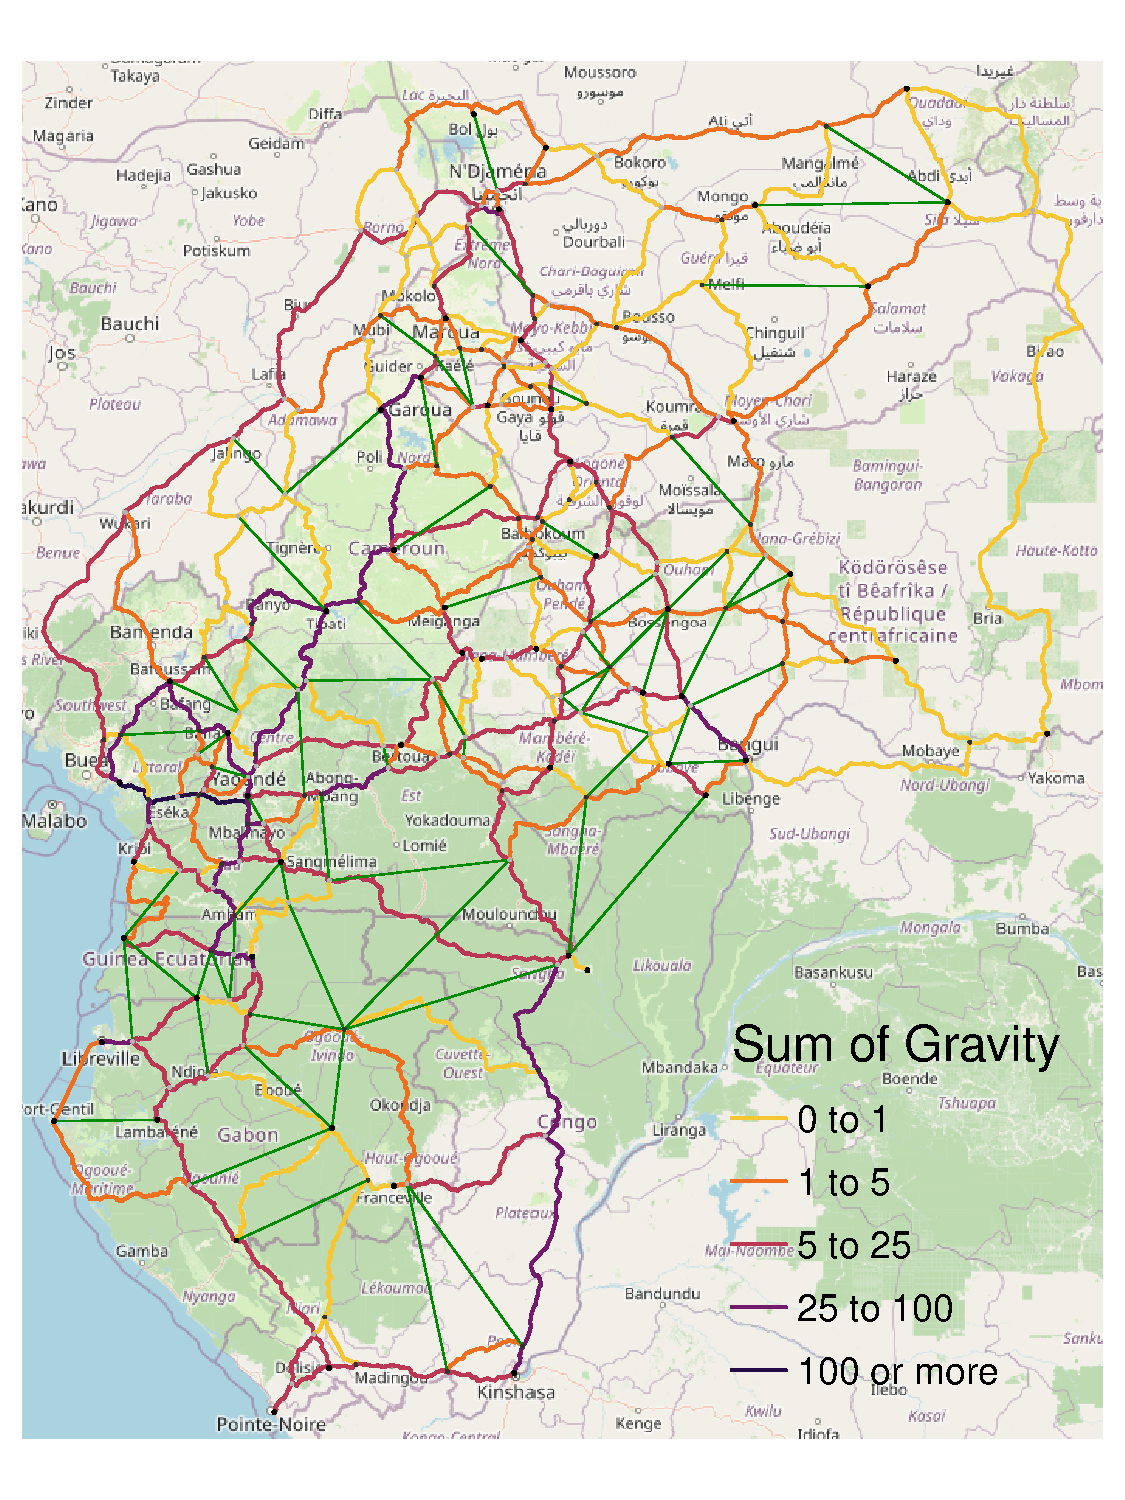
\includegraphics[width=0.48\textwidth]{"../figures/trans_CEMAC_network_actual_discretized_gravity_new_roads_real_edges.pdf"} &
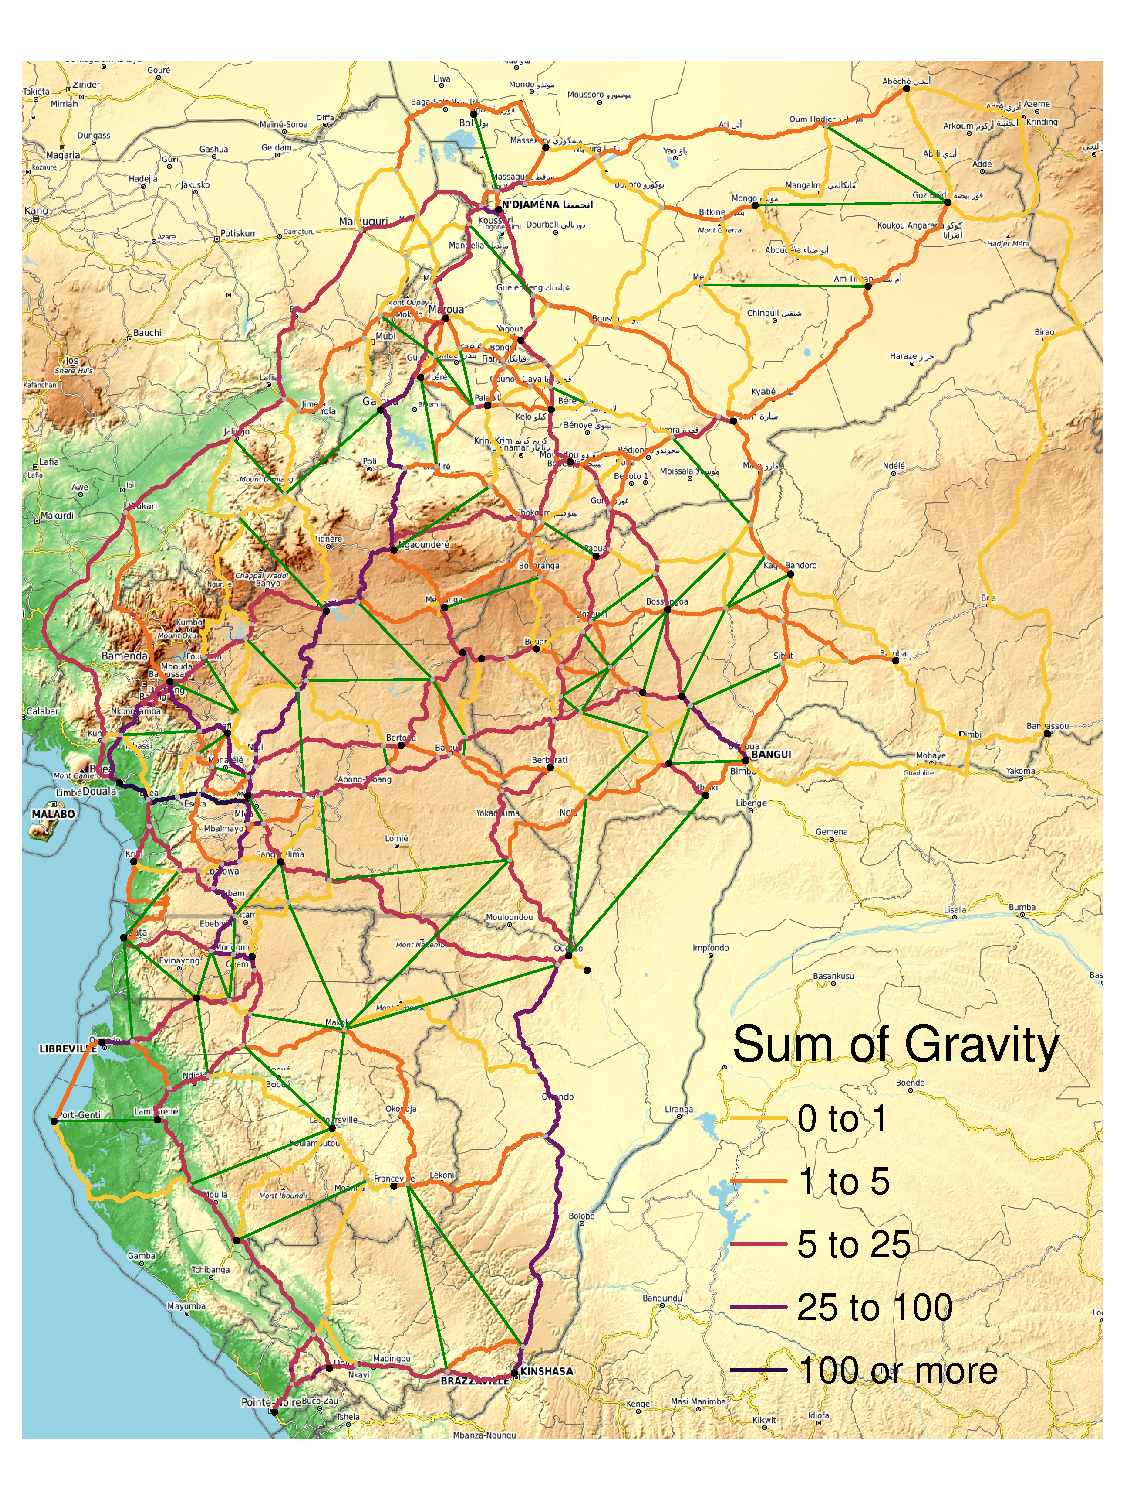
\includegraphics[width=0.48\textwidth]{"../figures/trans_CEMAC_network_actual_discretized_gravity_new_roads_OpenTopoMap.pdf"} \\ [-0.8em]
\end{tabular}
\raggedright
\scriptsize 
\emph{Notes:} Figure shows road network graph against a plain (LHS) and topographic (RHS) background map. The network is obtained from 1431 fastest car routes between 54 cities/agglomerations. Each route is assigned a 'Gravity' estimate amounting to the population (in thousands) of start and end city divided by the road distance in meters. The 'Sum of Gravity' is the sum across all routes using this segment in the network. It is a measure of expected traffic volume. The green lines indicate high-yield network extensions yielding $\geq$50\% reductions in road distance between adjacent nodes. % \\ \vspace{-5mm}
\end{figure}

To parameterize the graph, I add the populations of smaller agglomerations within 30km of these nodes to the node population count, excluding Nigerian agglomerations. CEMAC planners should not maximize welfare or market access in Nigeria. This yields 119 nodes with positive populations, of which 54 are the large cities routed from/to. According to the Africapolis 2025 projection, these nodes account for 80\% of the urban population of CEMAC.  \newline %, but only for 45\% of the total population in 2023 according to the World Development Indicators database. Since large cities generally exhibit higher productivities than small cities and rural populations, and, in the absence of a convincing way to measure productivity,\footnote{\citet{krantz2024optimal} in the appendix shows that nightlights per capita is not a convincing productivity measure. \vspace{-3mm}} I make the assumption that they also account for 80\% of the regions GDP. Readers who find this estimate high should note that road projects take 3-5 years to complete, the region's real GDP grew by 2.2\% annually over the last 10 years, and the urban population share, currently at 50\%, is increasing by 0.5 percentage points per year (own calculations using Africa Monitor data \citep{krantz2023africamonitor}). Thus, fixing the GDP of these nodes at 80\% of the region's 2023 GDP (in constant 2015 USD) is moderate for 2028-30.   \newline 

  To better distribute GDP across these nodes, I employ the high-resolution remotely sensed International Wealth Index (IWI) by \citet{lee2022high}.\footnote{\citet{krantz2024optimal} in the appendix shows that nightlights per capita is not a convincing productivity measure.} The index estimates asset-based household wealth on a scale from 0 to 100 based on a fixed set of household items recorded in DHS surveys. \citet{lee2022high} combine daylight satellite imagery and OpenStreetMap data in an iterative ML framework to predict the IWI from DHS surveys conducted in 25 Sub-Saharan African (SSA) countries since 2017 and obtain a cross-country $R^2$ of 91.7\%. Their predictions cover all populated areas at an effective resolution of 1.6km. \newline 
  
Additionally, I consider the total crop production of the region's 11 most important crops accounting for 80\% of total crop production from the SPAM dataset \citep{SPAM} ($\sim$10km spatial resolution). These crops and their share of total CEMAC crop production are CASS (19.8\%), PLNT (13\%), OILP (6.7\%), SUGC (6.7\%), MAIZ (6.6\%), ORTS (5.5\%), SORG (5.4\%), VEGE (4.5\%), YAMS (4.4\%), GROU (3.8\%), and BANA (3.5\%). Figure \ref{fig:IWISPAM} visualizes both measures. 

\begin{figure}[H] \vspace{-4mm}
\centering
\caption{\label{fig:IWISPAM} International Wealth Index and Crop Production at 10km Resolution}
\resizebox{\textwidth}{!}{
\begin{tabular}{@{}c@{}c@{}}
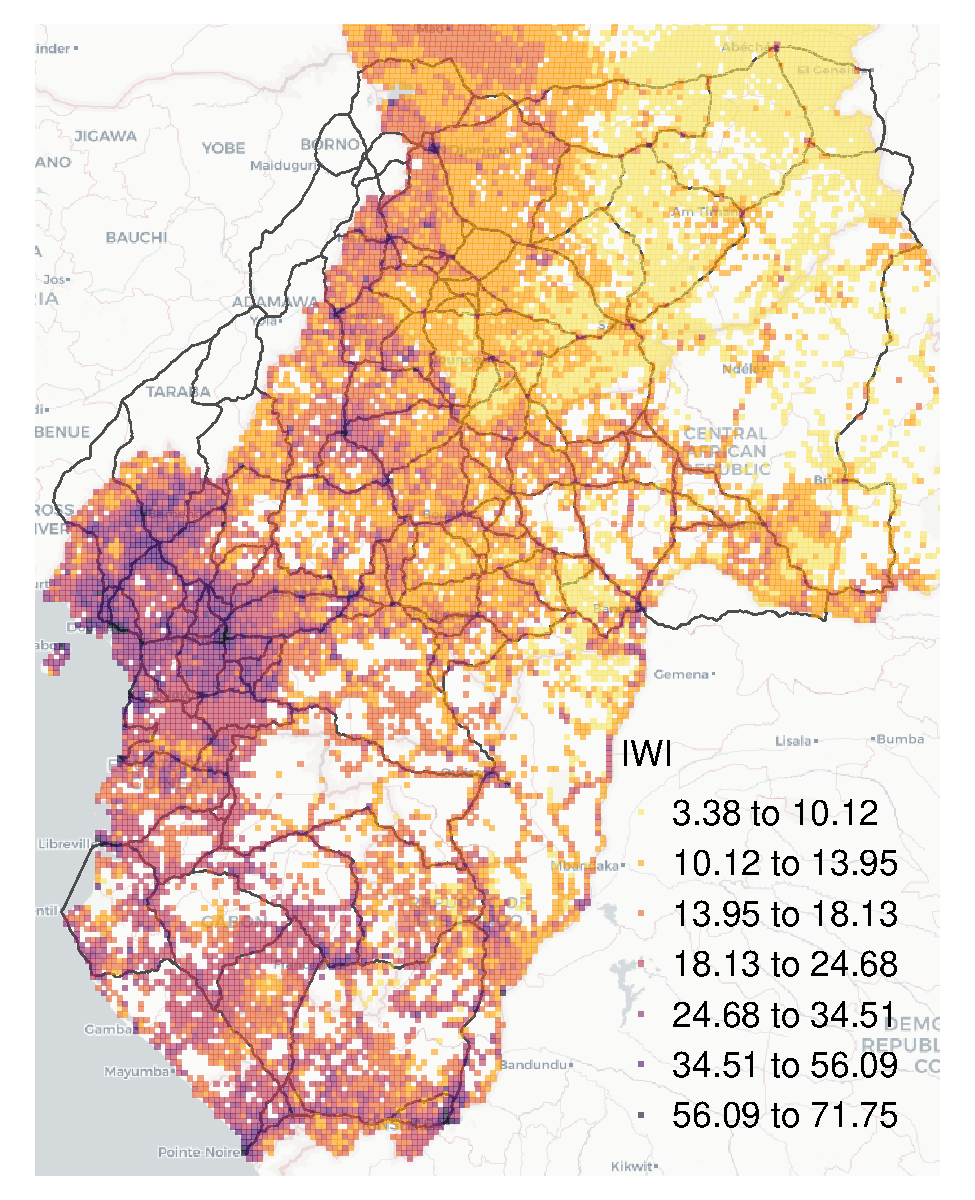
\includegraphics[width=0.5\textwidth, trim= {5mm 0 5mm 0}, clip]{"../figures/IWI_CEMAC_GRID.pdf"} & 
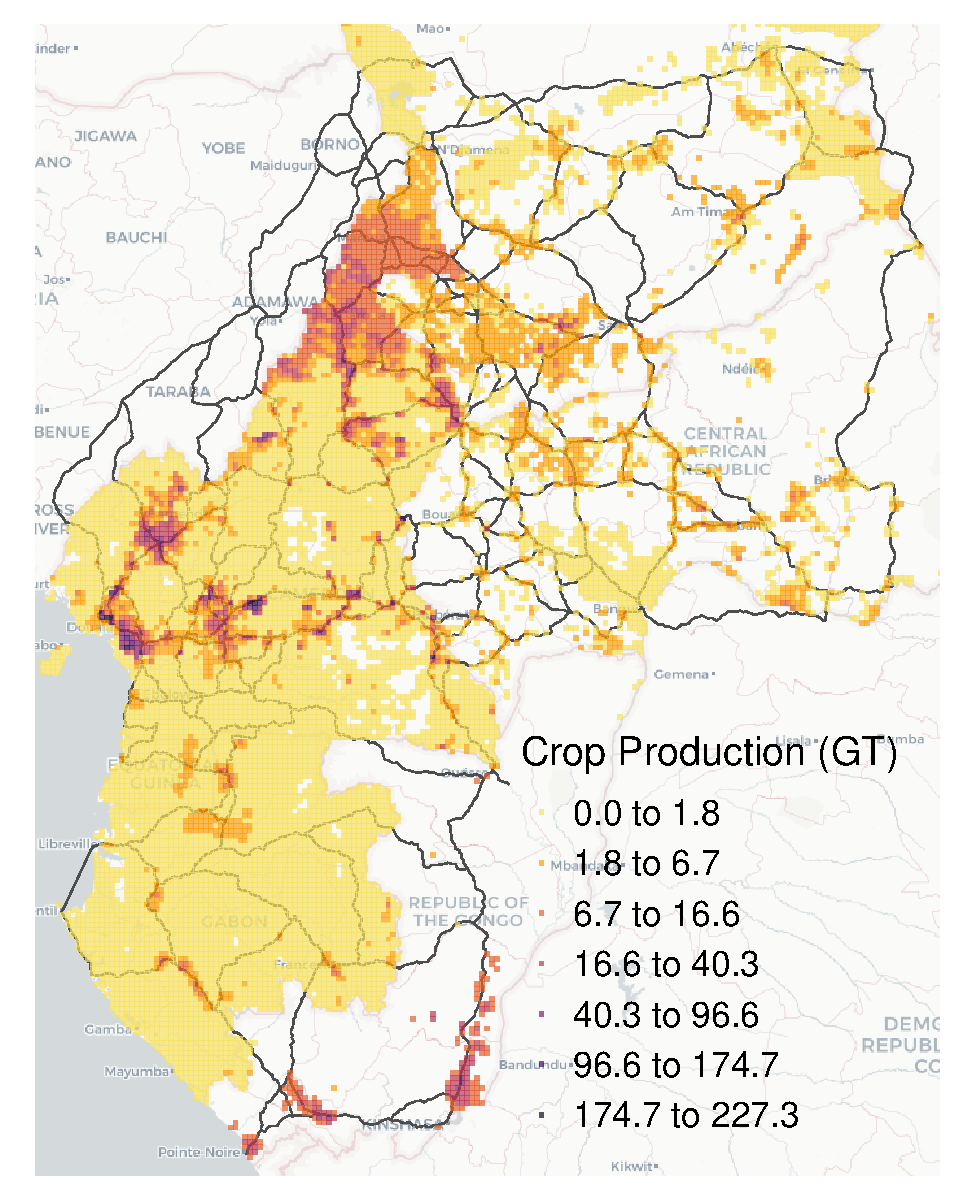
\includegraphics[width=0.5\textwidth, trim= {5mm 0 5mm 0}, clip]{"../figures/crops/SPAM_CEMAC_TOP80.pdf"}
\end{tabular}
}
\\\vspace{-2mm}
\raggedright
\scriptsize 
\emph{Notes:} Figure shows International Wealth Index \citep{lee2022high} and crop production of the region's 11 most important crops accounting for 80\% of total crop production \citep{SPAM}, aggregated to $\sim$10km diameter square cells.
\end{figure}

  To estimate node productivity, I take an inverse-distance-weighted average of all IWI estimates within 10km of each node (to give more weight to productive city centers). This average ranges from $\sim 65$ IWI points in port cities such as Port-Gentil, Douala, and Libreville to $\sim 10$ in some remote cities such as Baibokoum in Chad. I then multiply it with the node population to measure total wealth and use that to distribute 80\% of the region's real 2023 GDP, amounting to 72.7 billion 2015 USD (total GDP is \$90.9B USD'15), across the 119 populated nodes. \newline 
  
 Additionally, I compute an inverse-distance weighted sum of crop production of the region's 11 most important crops within 50km around each node, where the weight of cell $i$ is $1 - \delta_{i\leq 50km} / 50km$, i.e., 0 for fields 50km or more from the node and 1 for fields at the node. I then use this sum to distribute the remaining 20\% of the region's 2023 GDP, amounting to 18.2 billion 2015 USD, across nodes. This is appropriate as the share of the primary sector in GDP ranges from 2.9\% in Equatorial Guinea to 28.6\% in the Central African Republic, with Cameroon accounting for 46\% of CEMAC GDP and 45\% of the CEMAC population, at 16.7\%. Figure \ref{fig:GDPNet} summarizes this process.
 
\begin{figure}[H] \vspace{-3mm}
\centering
\caption{\label{fig:GDPNet} Composition of Total Production (GDP)}
\resizebox{\textwidth}{!}{
\begin{tabular}{@{}c@{}c@{}@{}c@{}}
Crop Production (20\%) & Population $\times$ IWI (80\%) & 2023 GDP (100\% $=$ 90.9B USD'15) \\ [-0.5em]
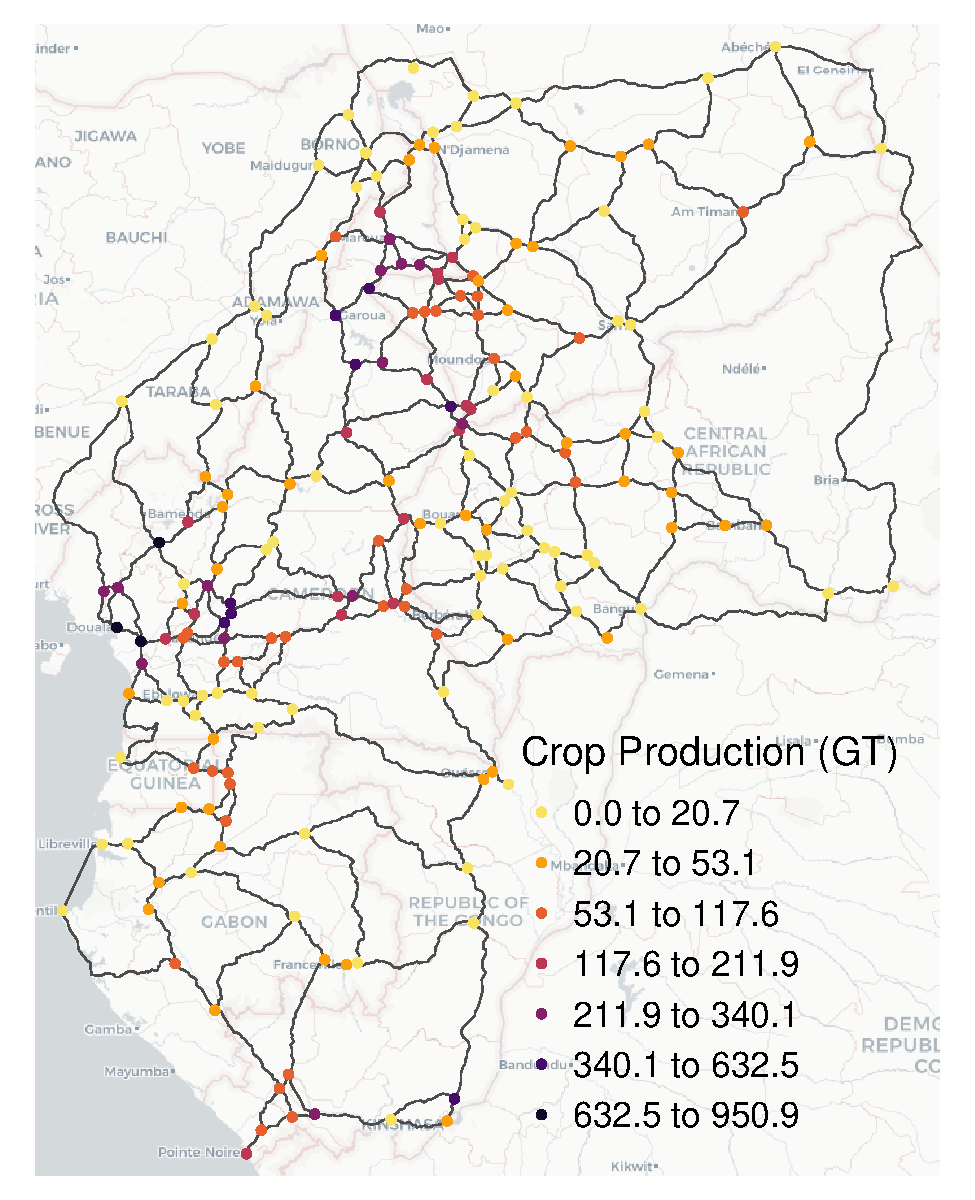
\includegraphics[width=0.38\textwidth, trim= {7mm 0 7mm 0}, clip]{"../figures/trans_CEMAC_network_SPAM_TOP80.pdf"} & 
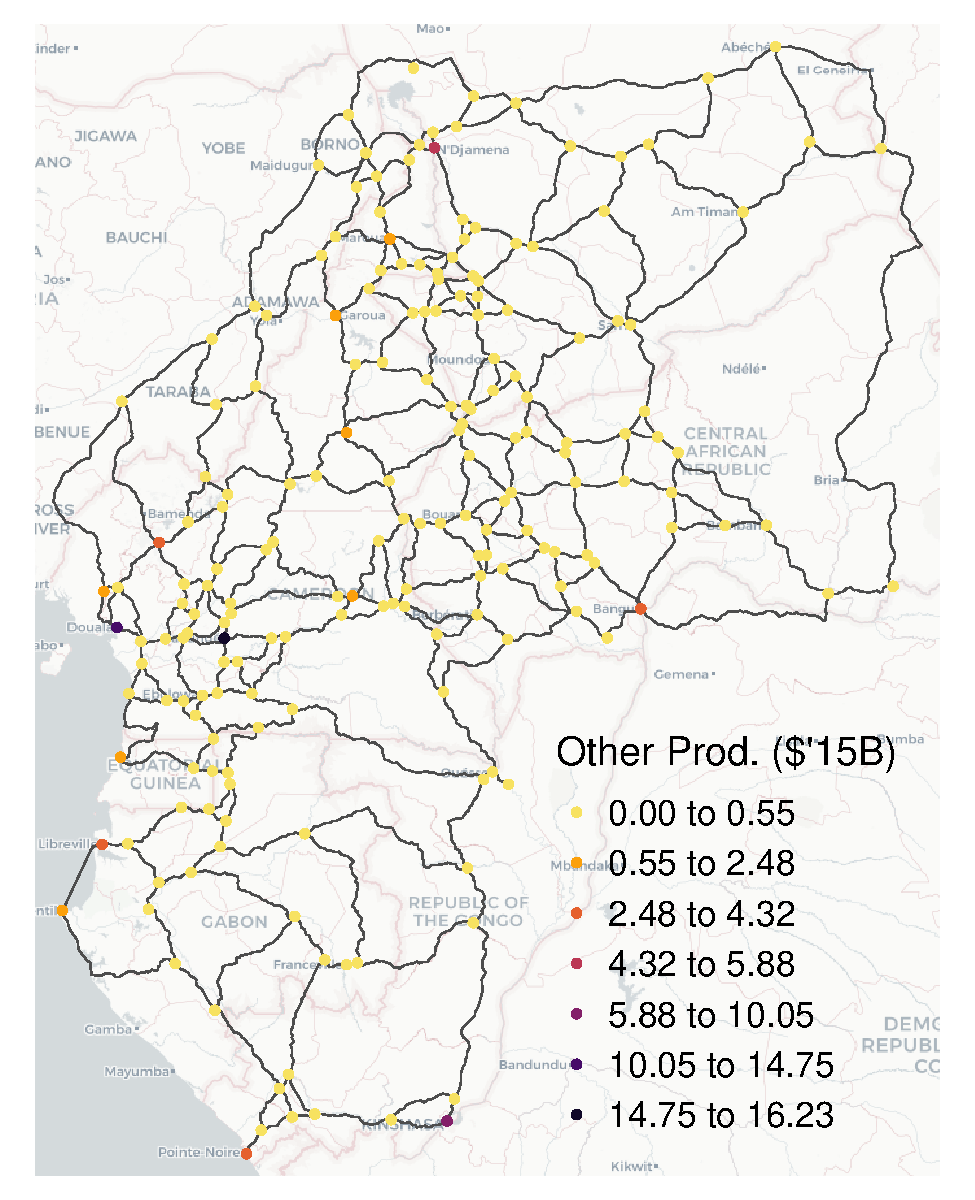
\includegraphics[width=0.38\textwidth, trim= {7mm 0 7mm 0}, clip]{"../figures/trans_CEMAC_network_GDP_other.pdf"} & 
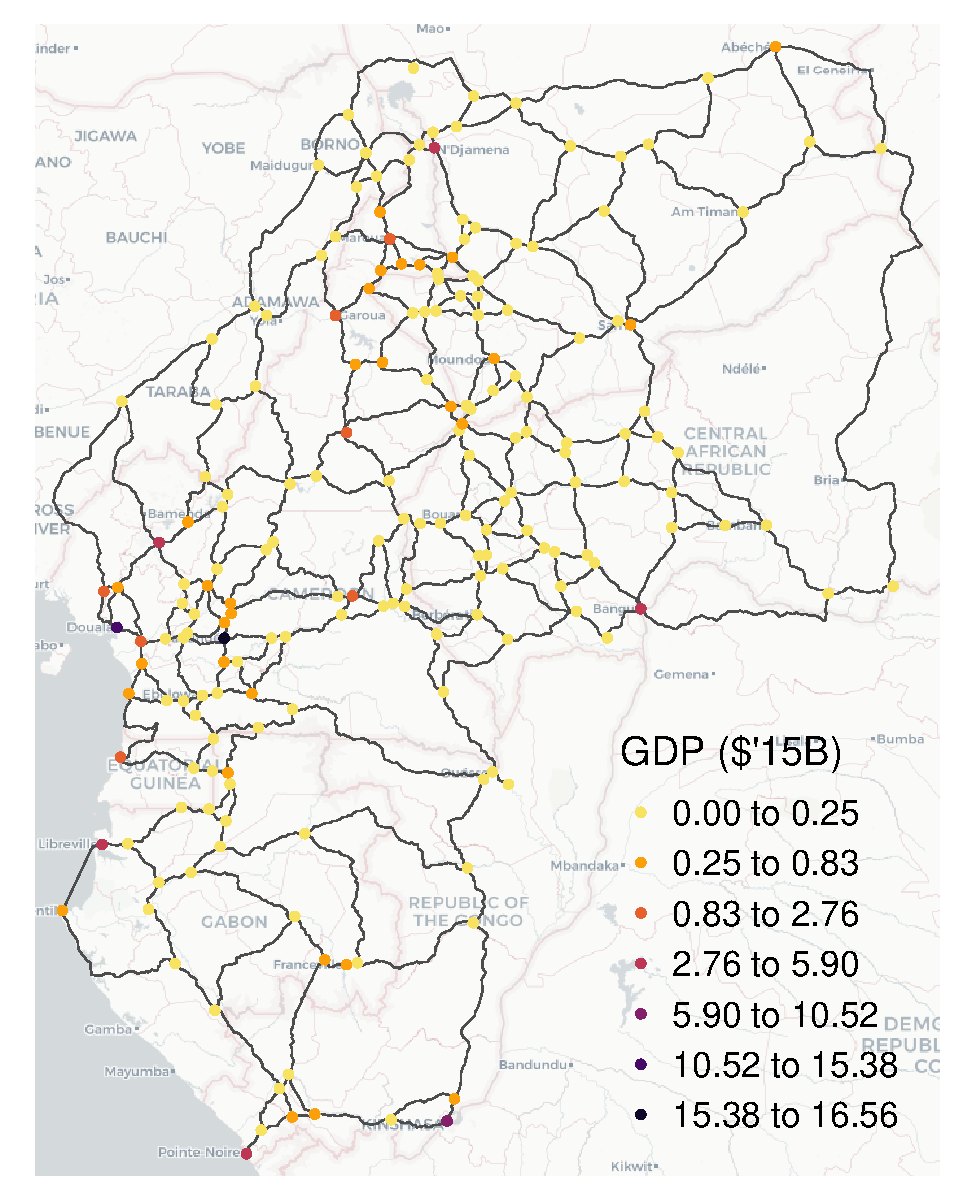
\includegraphics[width=0.38\textwidth, trim= {7mm 0 7mm 0}, clip]{"../figures/trans_CEMAC_network_GDP.pdf"}
\end{tabular}
}
\\\vspace{-2mm}
\raggedright
\scriptsize 
\emph{Notes:} Figure shows (inverse-distance weighted) production of top 11 crops within 50km radius of each node (LHS) and IWI within 10km around each node times node population (RHS). Both are combined to distribute GDP across nodes. \vspace{-5mm}
\end{figure}
  
I also take into account cross-border frictions following \citet{krantz2024optimal}. Figure \ref{fig:DB_TAB} visualizes them. The top panel shows the raw border compliance cost and time from the 2019 Doing Business Survey, and the bottom panel shows these converted to road distance and travel time, respectively, also taking into account documentary compliance times/costs. Evidently, and as visible in \citet{krantz2024optimal} Figures 8 and 9, border costs are high in the region, with a median cost of \$2272 and time of 411 hours, compared to the African median cost of \$1222 and time of 224 hours. 


  
  
\begin{figure}[H] \vspace{-2mm}
\centering
\caption{\label{fig:DB_TAB} World Bank Doing Business: Border Compliance Frictions in 2019}
\vspace{2mm}
\resizebox{\textwidth}{!}{
\begin{tabular}{cc}
Border Compliance Cost, Median: 2272\$  & Border Compliance Time, Median: 411h \\
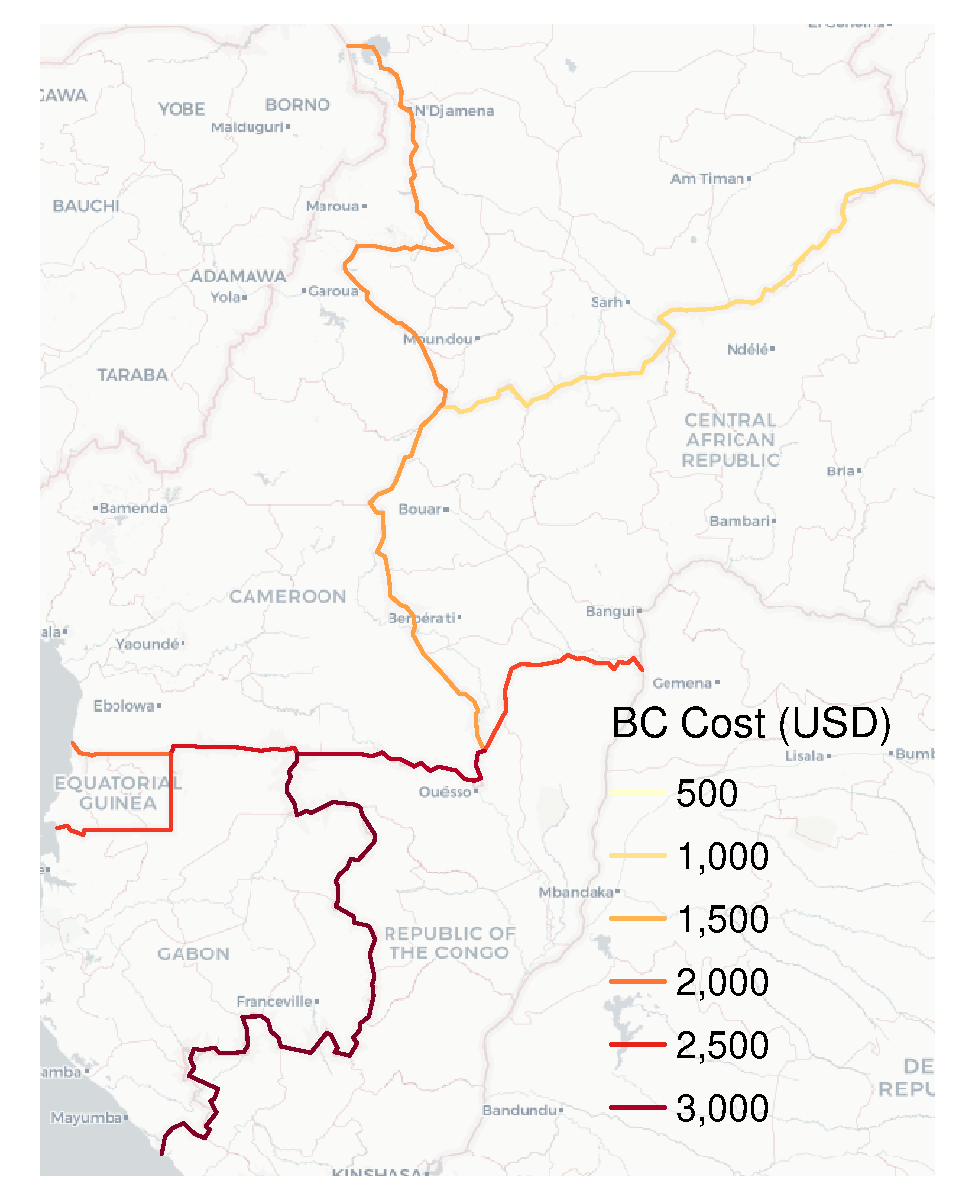
\includegraphics[width=0.5\textwidth, trim= {1cm 0 1cm 0}, clip]{"../figures/trade_costs/DBS_border_cost_usd_map.pdf"}  & 
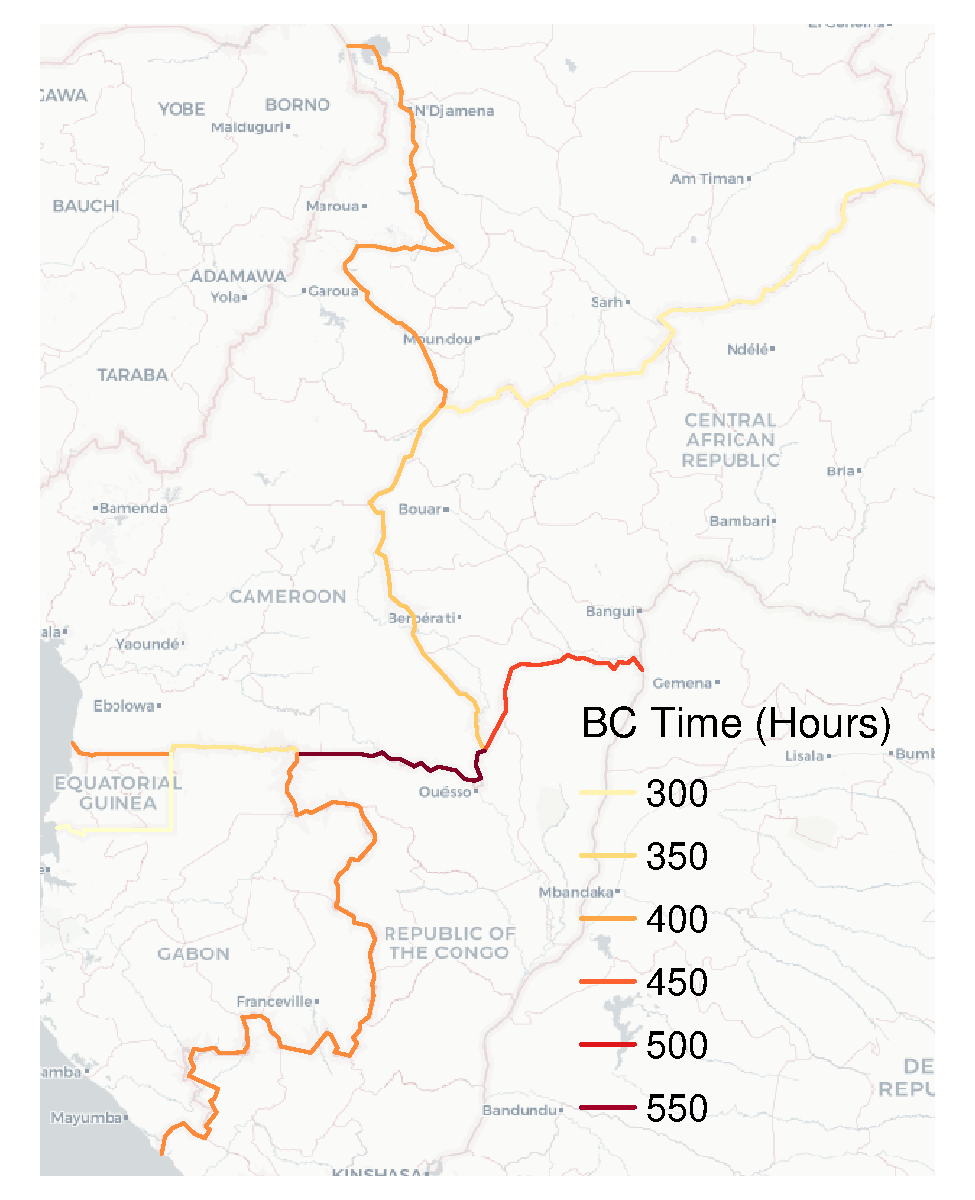
\includegraphics[width=0.5\textwidth, trim= {1cm 0 1cm 0}, clip]{"../figures/trade_costs/DBS_border_time_hours_map.pdf"}  \\ 
Distance-Equivalent Frictions, Median: 1724km & Time-Equivalent Frictions, Median: 127h \\
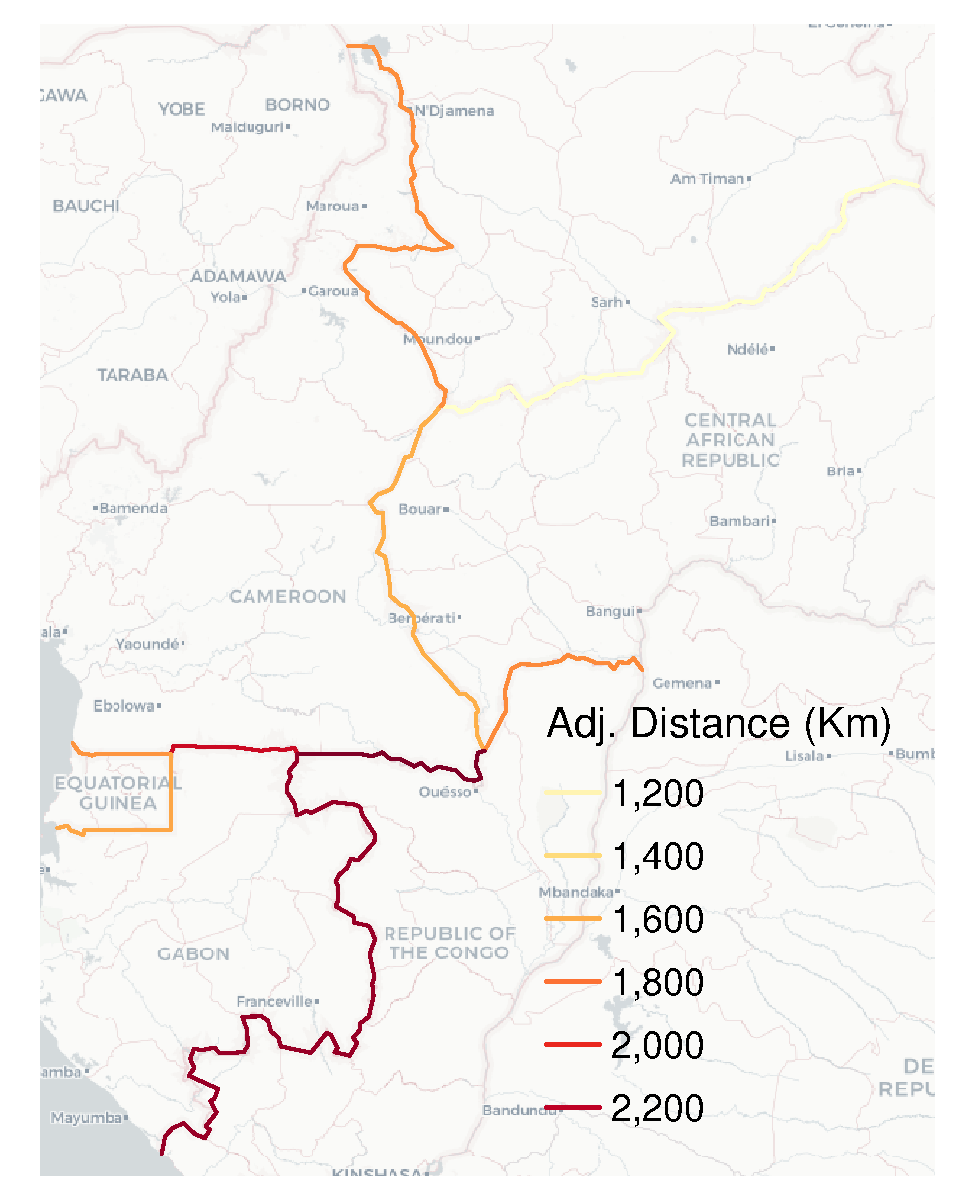
\includegraphics[width=0.5\textwidth, trim= {1cm 0 1cm 0}, clip]{"../figures/trade_costs/DBS_border_dist_km_adj_map.pdf"}  & 
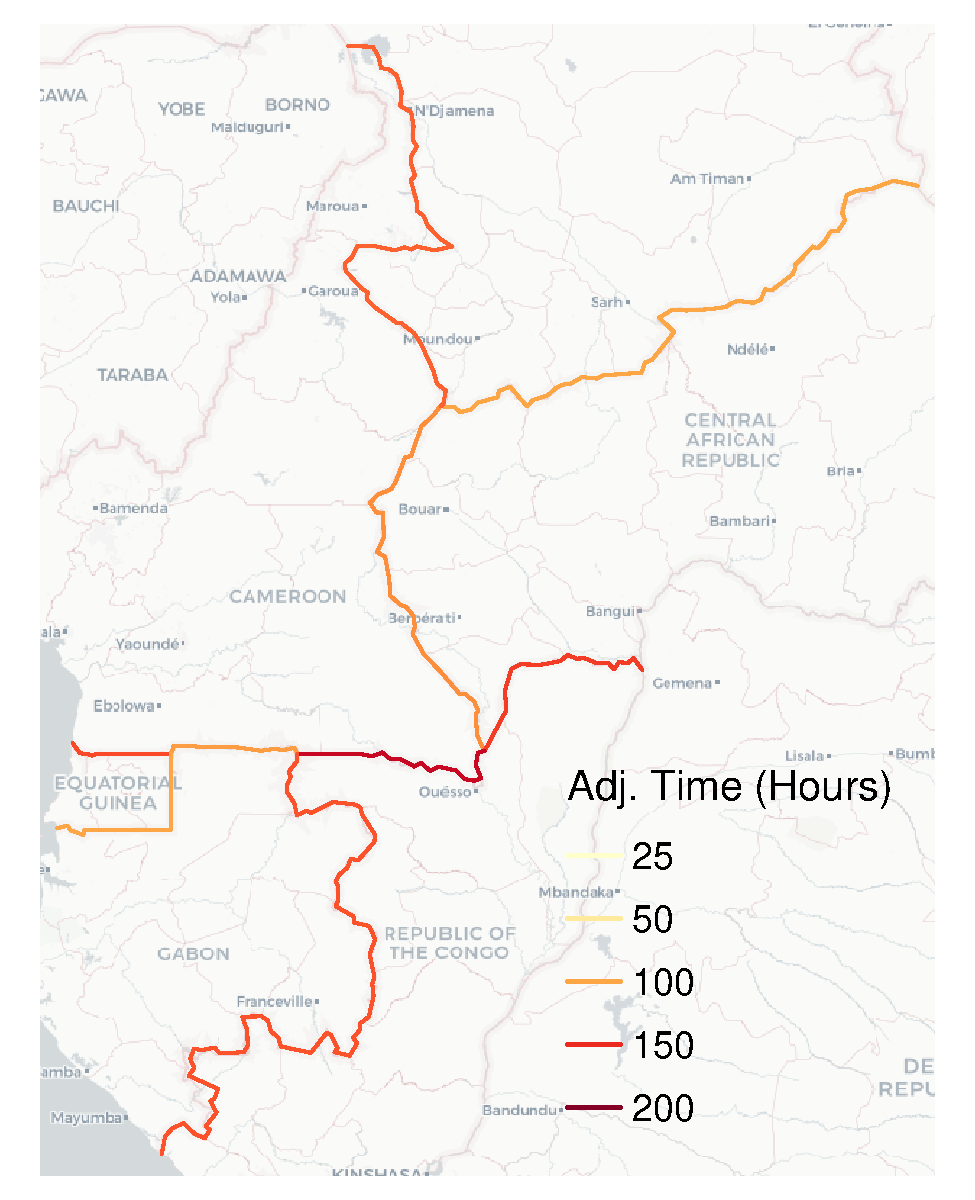
\includegraphics[width=0.5\textwidth, trim= {1cm 0 1cm 0}, clip]{"../figures/trade_costs/DBS_border_time_hours_adj_map.pdf"} \\ [-0.3em] 
\end{tabular}
} 
\raggedright
\scriptsize 
\emph{Notes:} Figure shows average (bi-directional) 2019 border compliance cost/time of trading a standardized product (top panel), and cost/time converted to road distance/travel time following \citet{krantz2024optimal}, i.e., dividing costs by 1.6 and documentary/border times by 10/4, respectively (bottom panel). \vspace{-5mm}
\end{figure}

\newpage
  
  
\section{Optimal Marginal Network Investments}

This section follows \citet{krantz2024optimal} Section 5 by first examining the returns to the proposed new links, then to upgrading existing links, followed by cost-benefit analysis, including joint scenarios. % To limit the scope of exposition, cost-benefit analysis is only done for the joint scenarios. 

\subsection{Building New Links}

The route efficiency (RE) of the network (NRE)\footnote{The spherical distance between two cities divided by road distance (RE) averaged across all 1431 routes (NRE).} is 0.667, and the RE of the average segment is 0.787. Assuming that the proposed segments (highlighted in green in Figure \ref{fig:ROADS}) also have a RE of 0.787 implies that building all of them increases NRE by 6.7\% to 0.712. When computing a weighted average of RE across routes using gravity (the product of origin and destination population divided by their geodesic distance) as weights, the weighted NRE measure is 0.683, and building all proposed segments raises it by 4.7\% to 0.715. As in \citet{krantz2024optimal}, the total NRE gain along all shortest routes can also be evaluated individually by segment. Figure \ref{fig:NRE_DA_TAN} shows the percentage gain in NRE from constructing each link. In the unweighted case, some large border crossing links in Congo, Gabon, Cameroon, and CAR yield high NRE gains, but with gravity weights, the most high yield links, with a NRE gain of more than 0.5\%, are in Equatorial Guinea. A look at any street map reveals that the country is not well connected to its neighbours.

\begin{figure}[h!] % \vspace{-3mm}
\centering
\caption{\label{fig:NRE_DA_TAN} Percentage Gain in Network RE from Constructing Each Proposed Link}
\vspace{2mm}
\begin{tabular}{cc}
Unweighted NRE Gain (\%) & Gravity Weighted NRE Gain (\%) \\ % Improved US-Grade Network\\
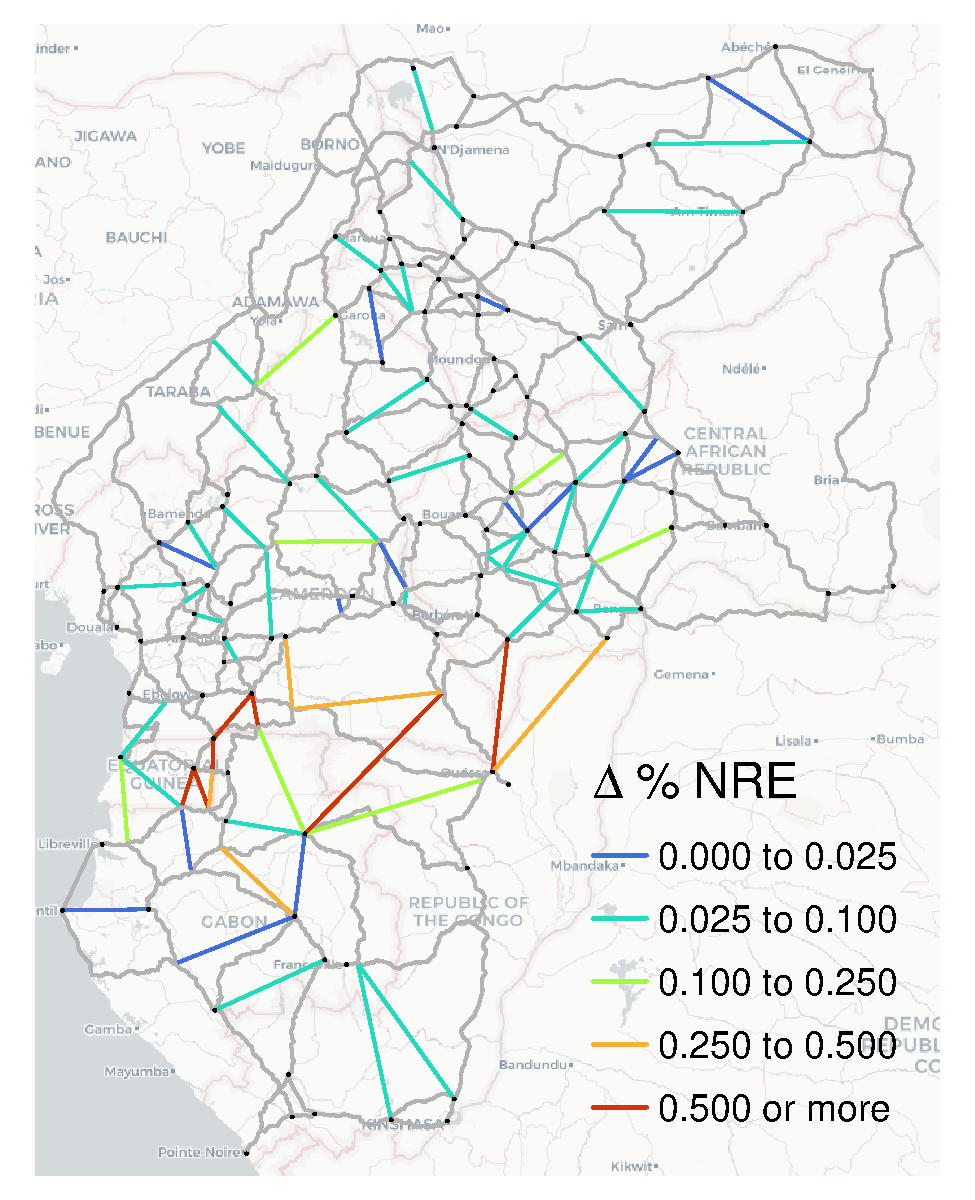
\includegraphics[width=0.48\textwidth]{"../figures/PE/trans_CEMAC_network_NRE_gain_perc.pdf"} &
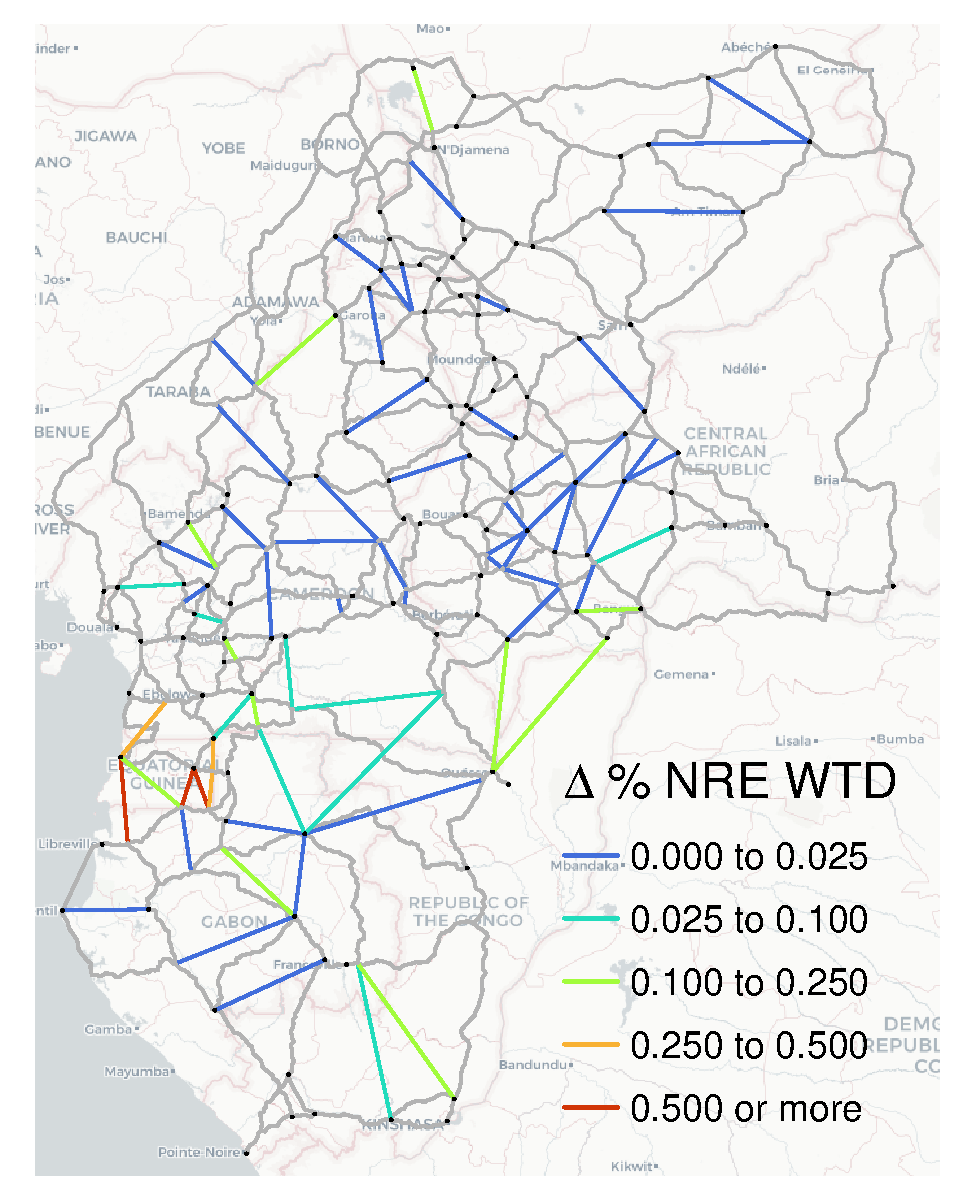
\includegraphics[width=0.48\textwidth]{"../figures/PE/trans_CEMAC_network_NRE_wtd_gain_perc.pdf"} \\ [-0.2em]
\end{tabular}
% \raggedright
\scriptsize 
\emph{Notes:} Figure shows (weighted) average route efficiency (NRE) gains across all trips from building a specific link/edge. 
 % \vspace{-1mm}
\end{figure}

Similarly, we can consider total market access (MA) implied by the network, where the MA of node $i$ is the sum of the estimated GDPs of all other nodes $j$ divided by their respective road distance along the fastest $i\to j$ route. The total network MA is then the sum of MA across all nodes. The total network MA is 28.3 billion USD'15 per km. Building all proposed links increases MA by 5\%. Using 2019 estimates of cross-border frictions from the final edition of the World Bank Doing Business surveys and translating documentary and border compliance time/cost into road time/distance, respectively, following \citet{krantz2024optimal}, reduces total MA to 19.6 billion USD'15 per km or 31\% smaller. The MA gain from all proposed links reduces to 3\%. Figure \ref{fig:MA_DA_TAN} shows the total MA gains from building each link with and without frictions and their ratio. Ostensibly, frictions reduce the value of new border-crossing links. The marginal gains from all links are lower under frictions as long as the route is fixed and transiting is less costly. \citet{krantz2024optimal} discusses other cases where traders can adjust their multi-country routes to minimize border costs, which I refrain from here as the CEMAC region is small. Following \citet{krantz2024optimal}, I set a 48h transit cost (24h per border) for transiting through 3rd countries. %, the focus should not be on the impact of border frictions except to make it clear that they should be removed as much as possible. 


\begin{figure}[H]  \vspace{-1mm}
\centering
\caption{\label{fig:MA_DA_TAN} Percentage Gain in Market Access (GDP) from Constructing Each Proposed Link}
\vspace{2mm}
\resizebox{\textwidth}{!}{
\begin{tabular}{@{}c@{}c@{}@{}c@{}} 
No Frictions & 2019 Doing Business Frictions & Ratio (Frictions/Frictionless) \\
\includegraphics[width=0.38\textwidth, trim= {0.9cm 0 0.9cm 0}, clip]{"../figures/PE/trans_CEMAC_network_MACR_gain_perc.pdf"} & 
\includegraphics[width=0.38\textwidth, trim= {0.9cm 0 0.9cm 0}, clip]{"../figures/PE/trans_CEMAC_network_MACR_gain_perc_bc.pdf"} & 
\includegraphics[width=0.38\textwidth, trim= {0.9cm 0 0.9cm 0}, clip]{"../figures/PE/trans_CEMAC_network_MACR_gain_bc_ratio.pdf"}
\end{tabular}
}
% \raggedright
\scriptsize 
\emph{Notes:} Figure shows total road-distance denominated MA gains measured (summed) across all trips from building a link. 
 % \vspace{-2mm}
\end{figure}

\subsection{Upgrading Existing Links}

The median link speed, taken from Google Maps without traffic awareness, is 60km/h, ranging from 6.2km/h for the slow ferry connection from Libreville to Port-Gentil, to 103km/h on the highway from Bata to Mongomo in Equatorial Guinea. Figure \ref{fig:ALS} shows the speed of each link. 

\begin{figure}[H]  \vspace{-2mm}
\centering
\caption{\label{fig:ALS} Average Link Speed}
\vspace{2mm}
\begin{tabular}{cc}
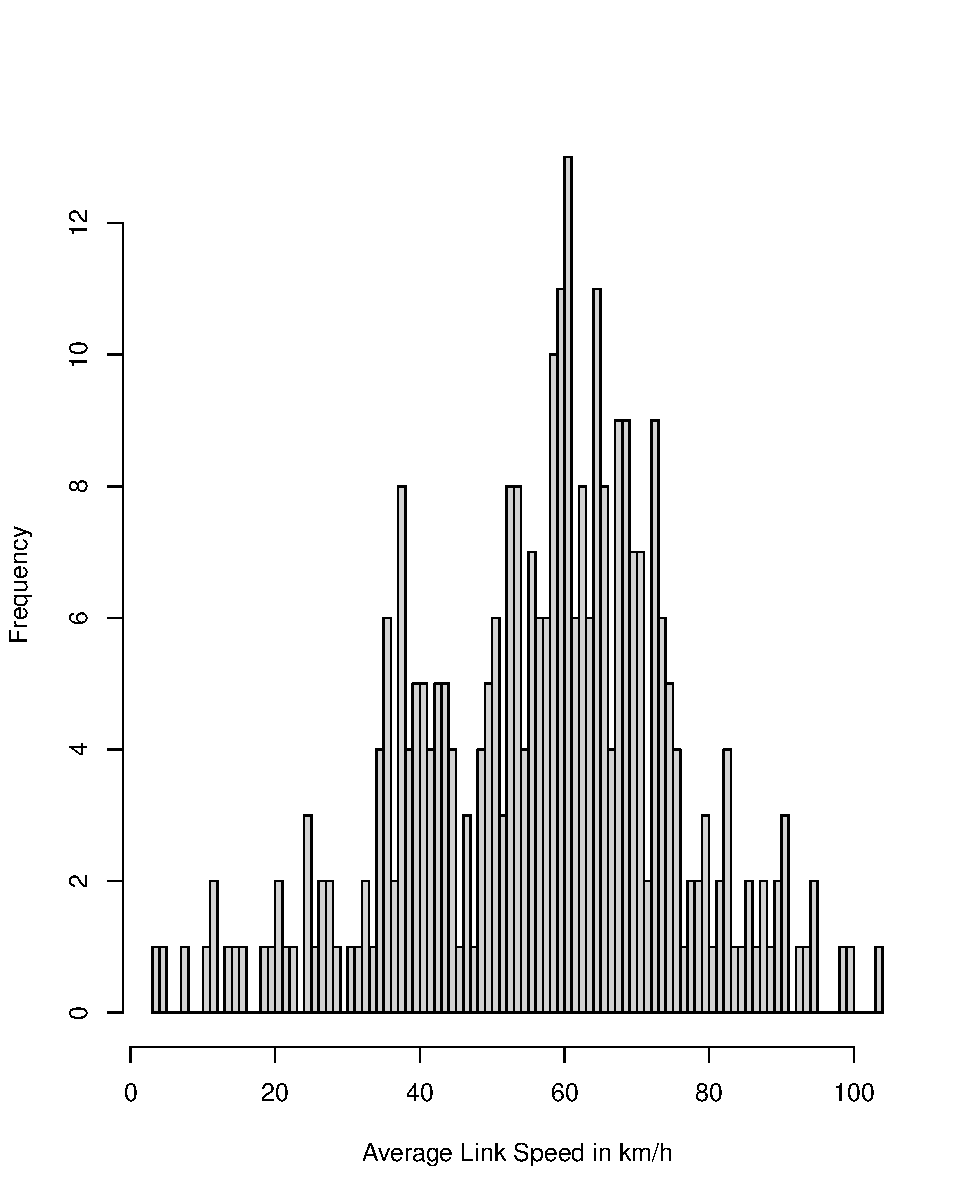
\includegraphics[width=0.48\textwidth, trim = {0 0.4cm 1.5cm 2.5cm}, clip]{"../figures/trans_CEMAC_network_average_link_speed_hist_google.pdf"} &
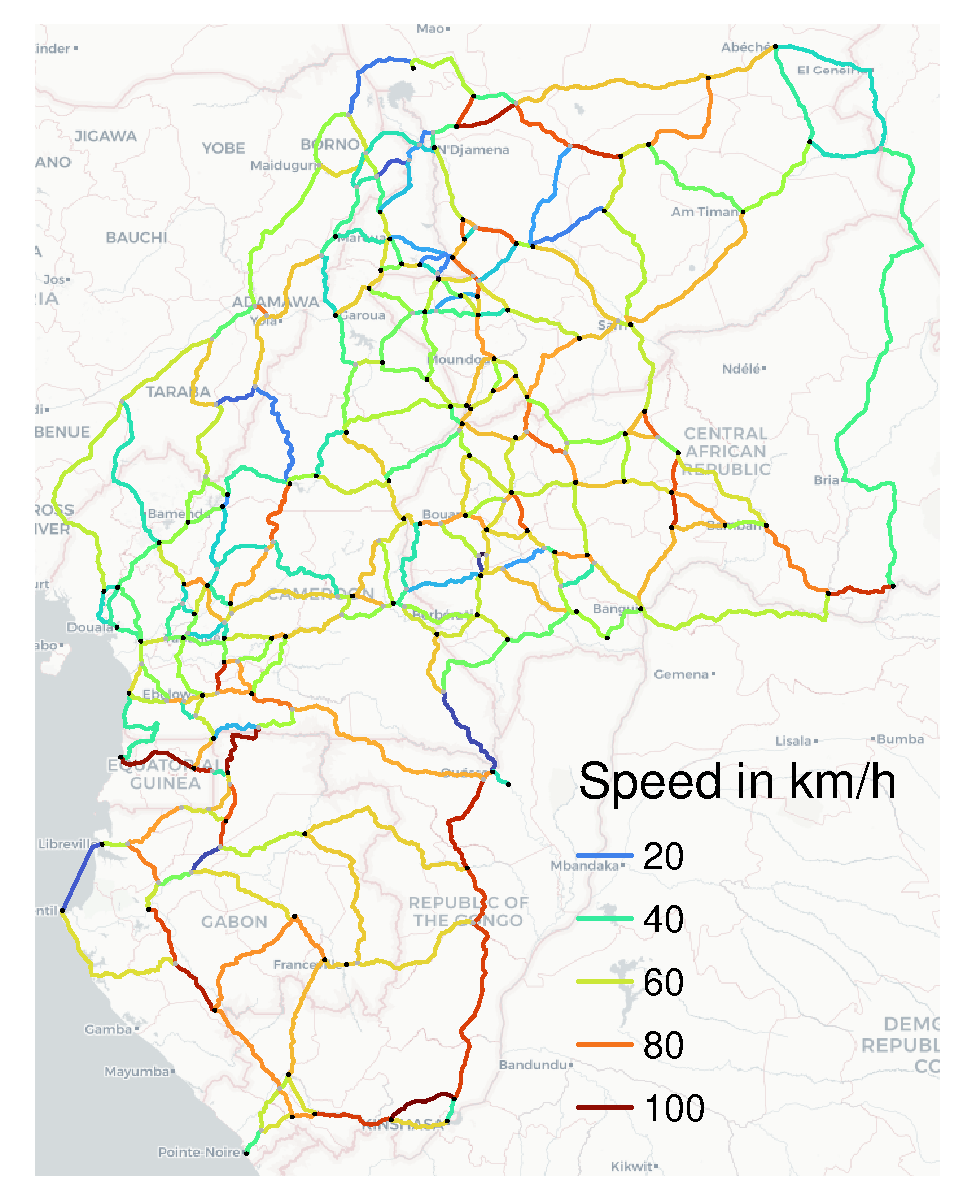
\includegraphics[width=0.48\textwidth]{"../figures/trans_CEMAC_network_average_link_speed_google.pdf"}  \\ % [-0.2em]
\end{tabular}
% \raggedright
\scriptsize 
\emph{Notes:} Figure shows the average speed along each link, estimated via Google Maps API without traffic awareness. 
\end{figure}

The total travel-time-denominated MA implied by the network is 26.5 billion USD'15 per minute. Upgrading all roads to allow travel speeds of 90km/h or above (which is the 97th percentile of the link-speed distribution) raises total MA by 63.8\%. Under border frictions, the MA drops to 15.3 billion USD'15 per minute or 42.2\% smaller, and the gains from upgrading all roads is 60.2\%.\newpage Figure \ref{fig:MA_TT} shows the gains from upgrading each link individually with/without border frictions, including their ratio. The ratio graph, in particular, shows that frictions reduce the gains from upgrading border-crossing links and links in rural areas near international borders.

% Total MA gains from building at 100km/h and upgrading 30.57% or 9.31 billion USD'15/min

\begin{figure}[H]  \vspace{-3mm}
\centering
\caption{\label{fig:MA_TT} Percentage Gain in Market Access from Upgrading Each Link to $\geq$90km/h}
\vspace{2mm}
\resizebox{\textwidth}{!}{
\begin{tabular}{@{}c@{}c@{}@{}c@{}} 
No Frictions & 2019 Doing Business Frictions & Ratio (Frictions/Frictionless) \\
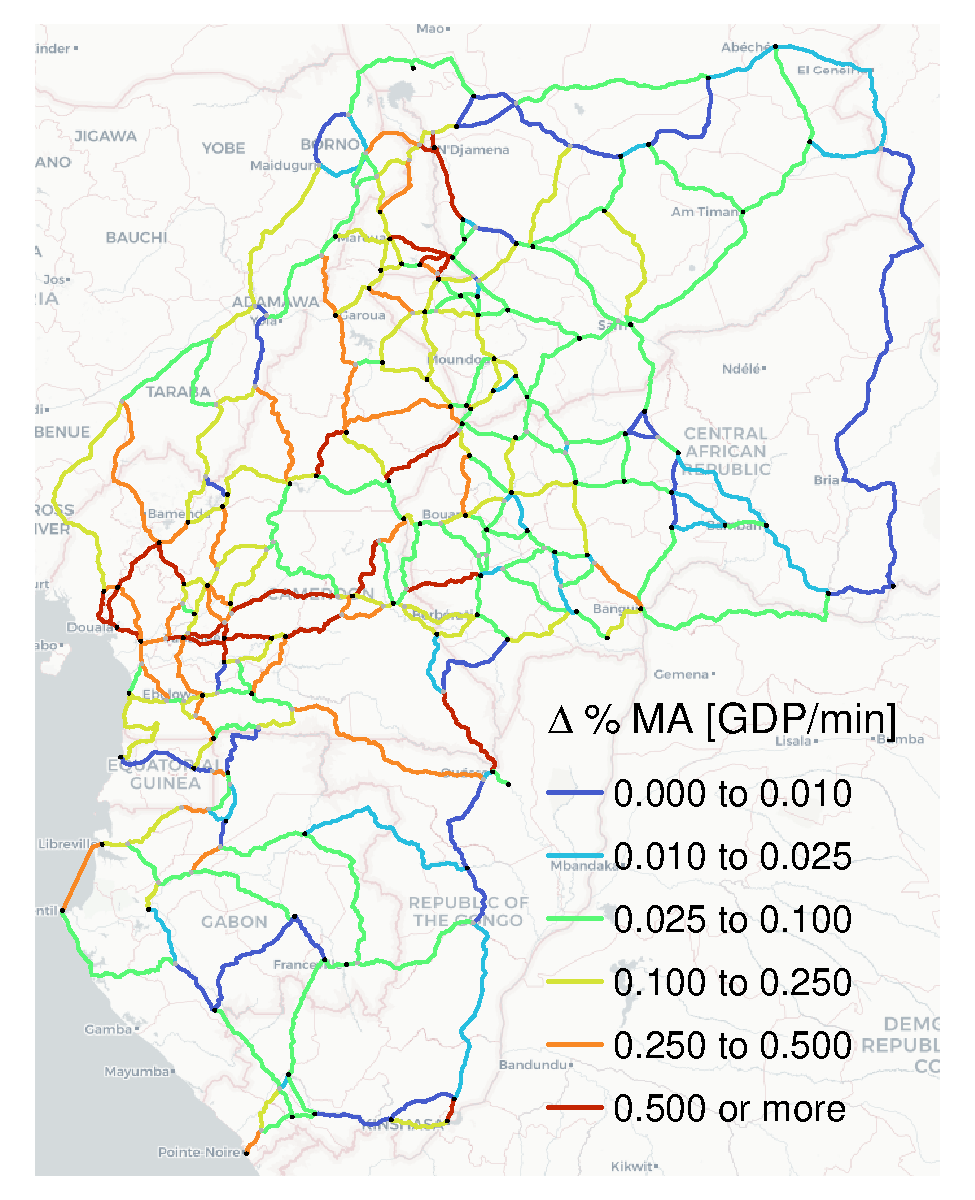
\includegraphics[width=0.38\textwidth, trim= {0.9cm 0 0.9cm 0}, clip]{"../figures/PE/trans_CEMAC_network_MACR_90_min_speed_perc_google.pdf"} & 
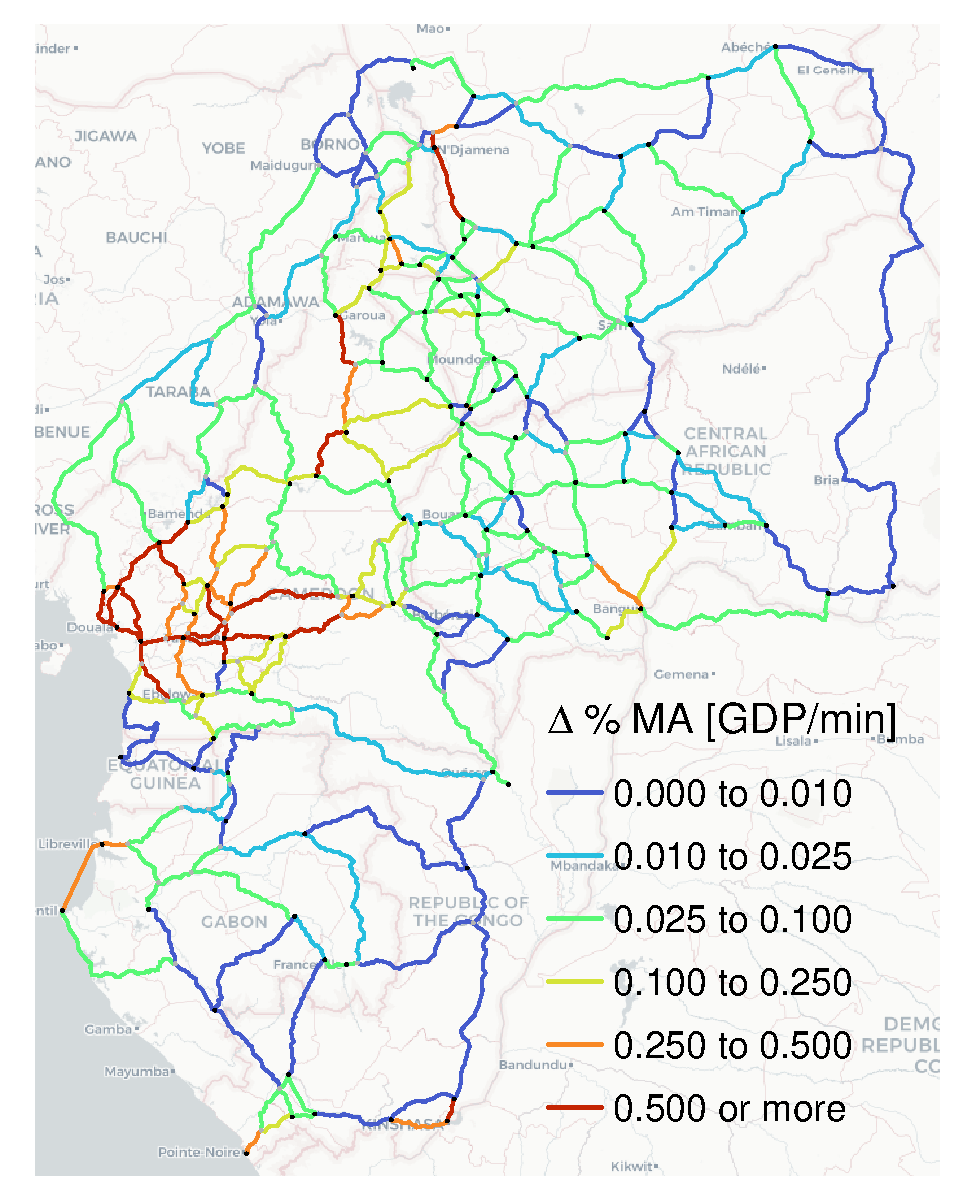
\includegraphics[width=0.38\textwidth, trim= {0.9cm 0 0.9cm 0}, clip]{"../figures/PE/trans_CEMAC_network_MACR_90_min_speed_bt_perc_google.pdf"} & 
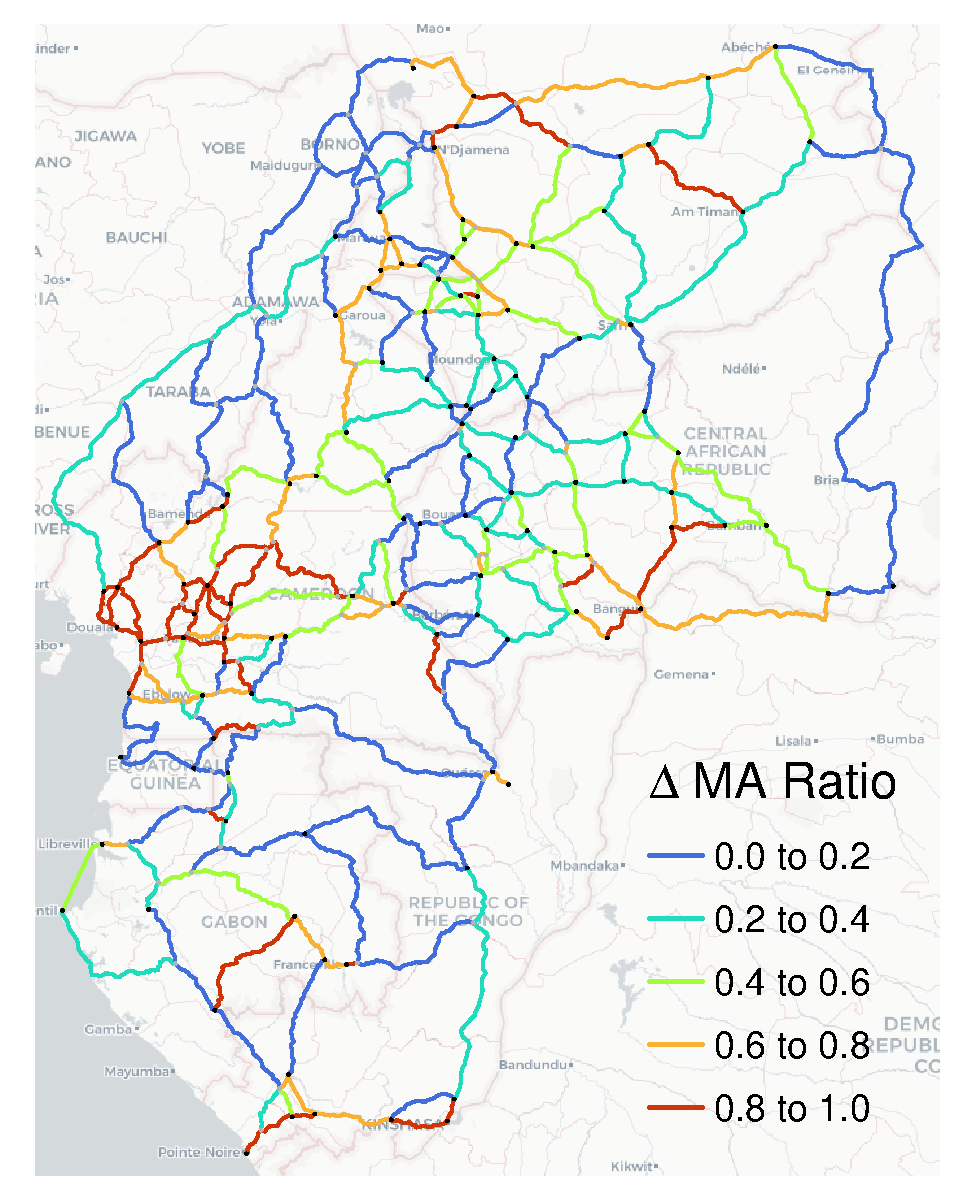
\includegraphics[width=0.38\textwidth, trim= {0.9cm 0 0.9cm 0}, clip]{"../figures/PE/trans_CEMAC_network_MACR_90_min_speed_bt_ratio_google.pdf"}
\end{tabular}
}
\raggedright
\scriptsize 
\emph{Notes:} Figure shows total travel-time-denominated MA gains measured (summed) across all trips from upgrading a link to allow travel speeds of $\geq$90km/h. \\ \vspace{-2mm}
 % \vspace{-2mm}
\end{figure}

Ostensibly, upgrading links in the populated areas of Cameroon, the by far largest economy among the 6, yields the greatest MA returns, especially under border frictions. Without frictions, better connecting the economic center of Cameroon up north and east also yields high MA gains.  

\subsection{Border Post Optimization}

I also simulate the effect of reducing the border cost at specific borders, measuring the change in total MA, taking into account traders' decisions to take the fastest route. Following \citet{fontagne2023trade}, I consider a 50\% border cost/time reduction, gauged to be the effect of replacing a traditional border post with a one-stop border post. However, the region's median road-time equivalent border cost is 127h, which is very high even in African comparison where the median is 76h, coming as low as 5h for the Namibia-Botswana and Mozambique-Eswatini borders. Thus, I also consider a scenario where the border cost is reduced to 12h regardless of the original cost, amounting to a $\sim$90\% reduction from the regional median. For reference, I also consider a 100\% reduction where the respective border cost is set to zero. Figure \ref{fig:UG_bpopt} reports the results.


\begin{figure}[H] \vspace{-3mm}
\centering
\caption{\label{fig:UG_bpopt} Border Post Optimization (Border Time Reduction)}
\vspace{2mm}
\resizebox{\textwidth}{!}{
\begin{tabular}{@{}c@{}c@{}@{}c@{}} 
 50\% \citep{fontagne2023trade} & To 12h (90\% from median) & 100\% \\
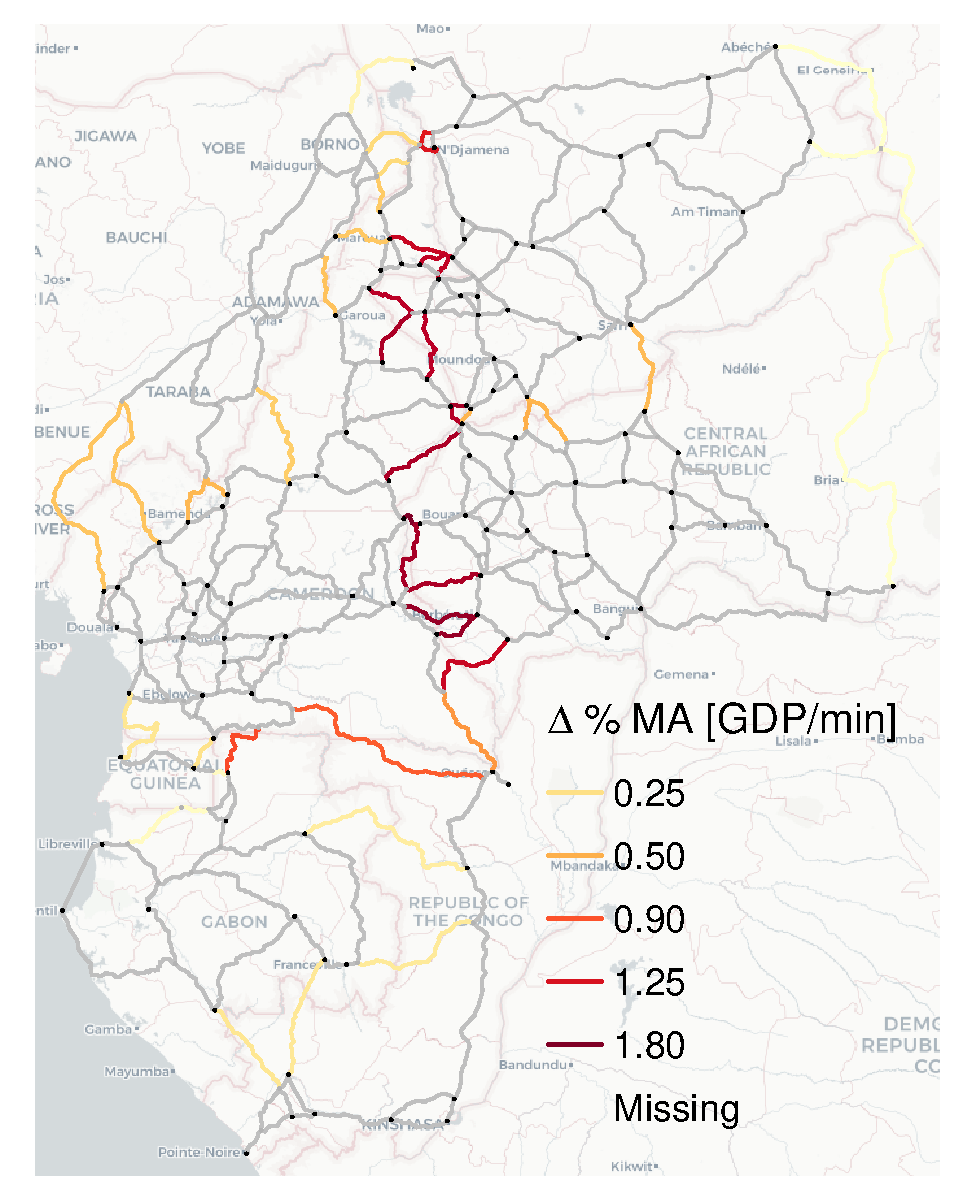
\includegraphics[width=0.38\textwidth, trim= {0.9cm 0 0.9cm 0}, clip]{"../figures/PE/trans_CEMAC_network_MACR_bt_50perc_red_perc_google.pdf"} & 
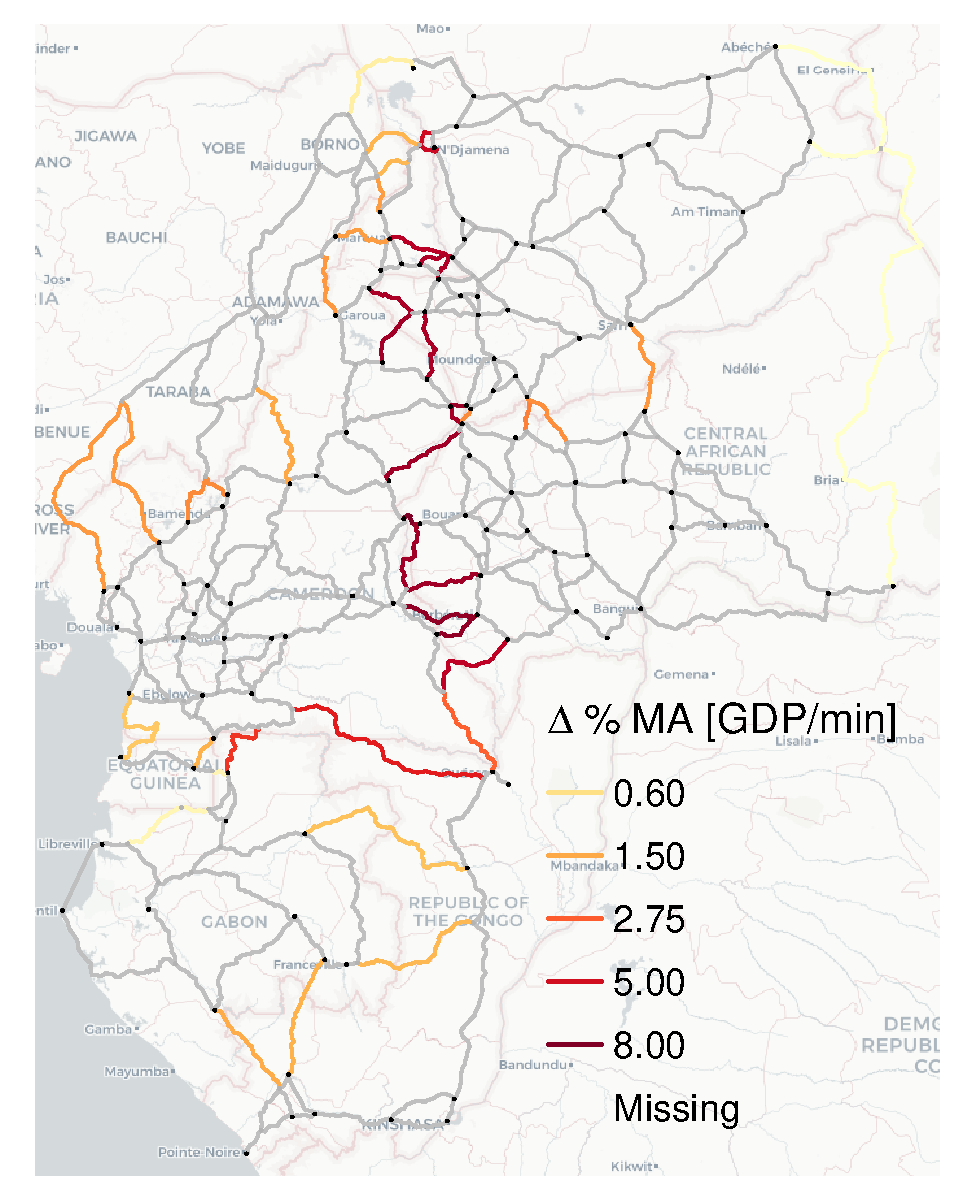
\includegraphics[width=0.38\textwidth, trim= {0.9cm 0 0.9cm 0}, clip]{"../figures/PE/trans_CEMAC_network_MACR_bt_90percto12h_red_perc_google.pdf"} & 
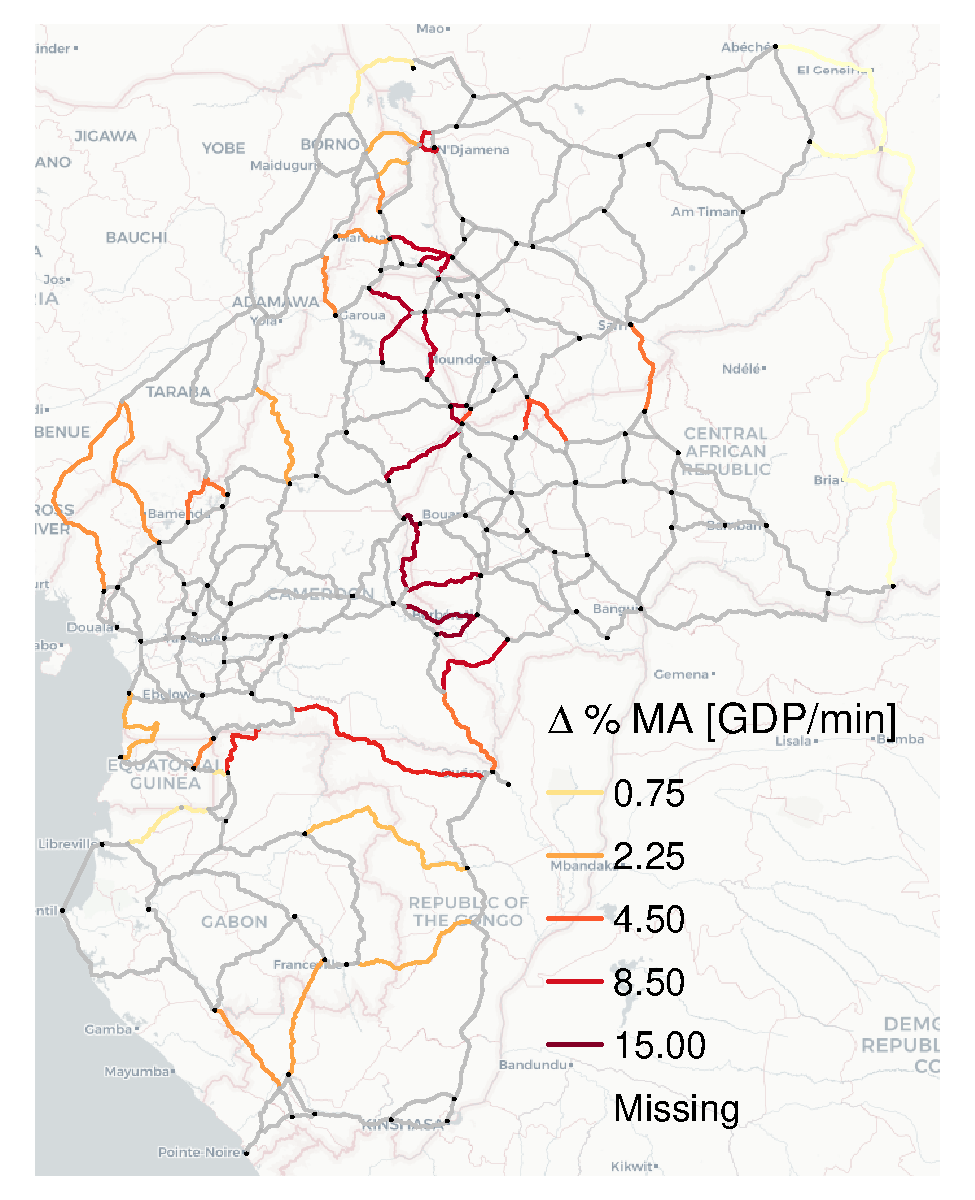
\includegraphics[width=0.38\textwidth, trim= {0.9cm 0 0.9cm 0}, clip]{"../figures/PE/trans_CEMAC_network_MACR_bt_100perc_red_perc_google.pdf"}
\end{tabular}
}
\\\vspace{-2mm}
\scriptsize 
\emph{Notes:} Figure shows the marginal MA gain from reducing border costs along on individual border-crossing links. \\\vspace{-1cm}
\end{figure}

In all three scenarios, reducing frictions at the border into Cameroon, the region's largest economy, yields the highest marginal MA gains of up to 1.8\% per border in the 50\% reduction case, 8.1\% in the reduction to 12h road-time equivalent case, and 15.7\% in the elimination case. The gains along any border differ across links depending on their navigational significance, i.e., how many traders can reroute along a least-cost path using this link. The most critical border yielding the highest gain in all scenarios is the border between Cameroon and CAR at Garoua-Boulai. 


\subsection{Cost-Benefit Analysis and Package Selection}

To decide which roads to invest in, the cost of building/upgrading roads must be taken into account. Following \citet{krantz2024optimal}, which in turn follows \citet{collier2016cost} using the updated (2018) Road Cost Knowledge System (ROCKS) database, I allow for heterogeneity in road construction costs. The median cost of a 2-lane highway in SSA is \$611K/km (2015 USD). This is consistent with recent data from the CEMAC region, yielding a median cost of \$614K/km and a median rehabilitation cost of \$356K/km. Following \citet{fajgelbaum2020optimal} and \citet{graff2024spatial}, I consider average returns to ruggedness and distance, as well as population, using coefficients averaged across different specifications in \citet{collier2016cost}. \citet{collier2016cost} also analyze the effects of conflict on road construction costs and find that costs are 30\% higher in conflict states (conflicts involving the government). I instead create a link-level continuous conflict measure $\Omega_j$ as the inverse-distance weighted sum of the square root of the fatality count across all ACLED conflicts within 50km of each link between 2018 and 2024. Specifically, for each link $j$ and qualifying conflict $k$
\begin{equation} \label{eq:conf}
\Omega_j = \sum_{k} \frac{50km-\delta_{kj}}{50km} \sqrt{\text{Fatalities}_k}\quad \forall\ k\ \text{where}\ \delta_{kj}\leq 50km\ \text{and}\  year(k)\geq 2018.
\end{equation}
In line with \citet{collier2016cost}'s treatment of continuous variables, I take the natural log of $\Omega_j$, and find that it ranges between 0 and 7.5, with a median of 2.84. Thus, since \citet{collier2016cost}'s dummy coefficient is 0.3, I assign a coefficient of $0.3/2.84\approx 0.1$. My road cost equation is thus
\begin{equation} \label{eq:COST}
\ln\left(\frac{\text{cost}}{km}\right) = \ln(X) -0.11 (\text{dist} > 50km) + 0.12 \ln(\text{rugg}) + 0.085 \ln\left(\frac{\text{pop}}{km^2}\right)+ 0.1 \ln(\Omega_j),
\end{equation}
where $X$ = 120,000 for new roads, $X$ = 101,600 for upgrades, $X$ = 64,600 for mixed works, and $X$ = 28.400 for resurfacing as in \citet{krantz2024optimal}. The first part is taken from Eq. (21) of \citet{fajgelbaum2020optimal}, the population coefficient follows \citet{collier2016cost} and \citet{krantz2024optimal}. The 120,000 USD/km constant makes the mean cost/km across all existing African links (excluding $\ln(\Omega_j)$) approximately equal to \$611K/km. The other thresholds adjust for different kinds of upgrading costs following \citet{krantz2024optimal}: (1) roads with speeds $<$60km/h require an upgrade at average cost of \$513K /km; (2) roads with speeds 60-79km/h require mixed works at average cost of \$326K/km; (3) roads with speeds 80-90km/h require resurfacing at \$143K/km on average. 

\begin{figure}[H] \vspace{-1mm}
\centering
\caption{\label{fig:RUGG_POP} Ruggedness and Population Density within 3km Buffer $+$ Conflict Incidence ($\Omega_j$)}
\vspace{2mm}
\resizebox{\textwidth}{!}{
\begin{tabular}{@{}c@{}c@{}@{}c@{}}
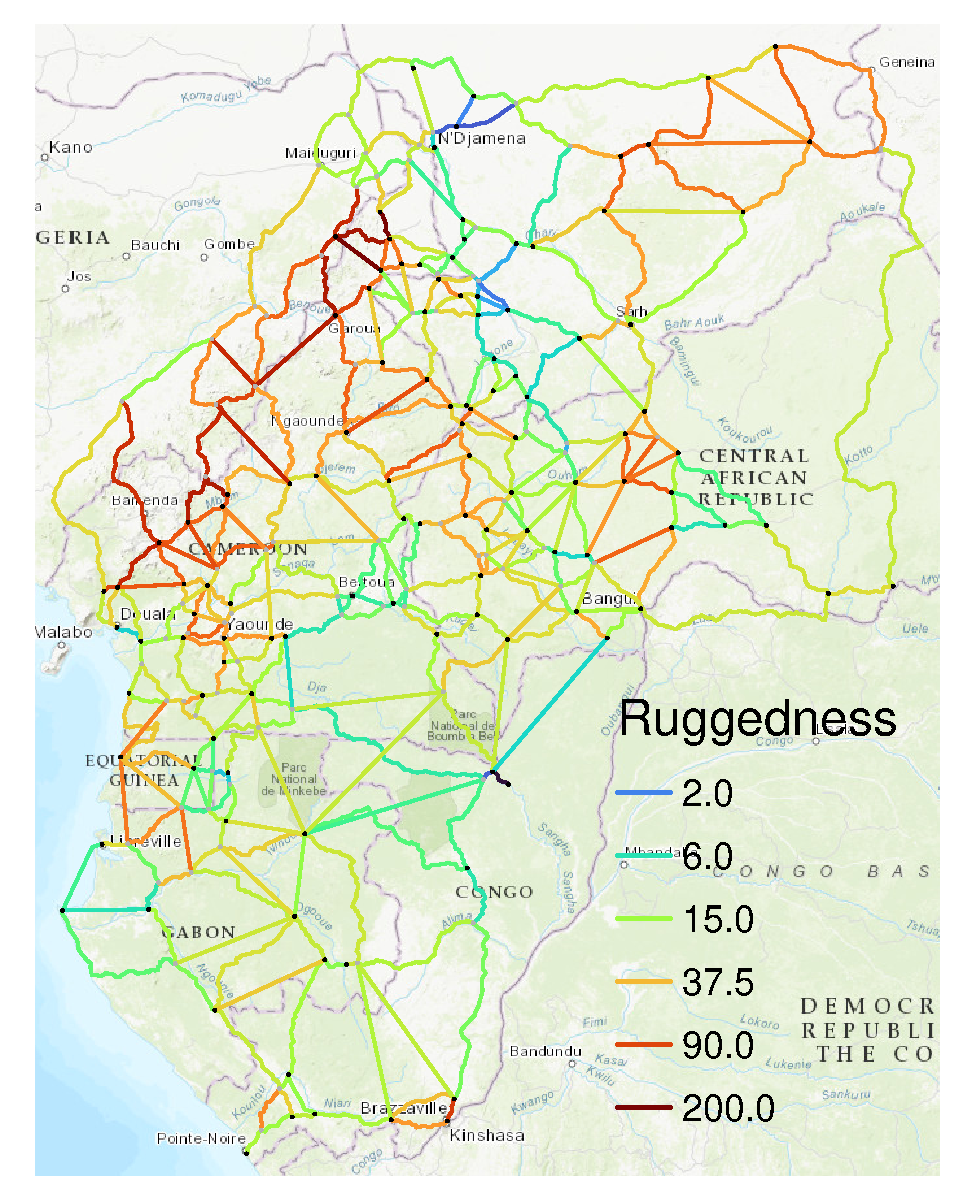
\includegraphics[width=0.38\textwidth, trim= {1cm 0 1cm 0}, clip]{"../figures/trans_CEMAC_network_rugg.pdf"} & 
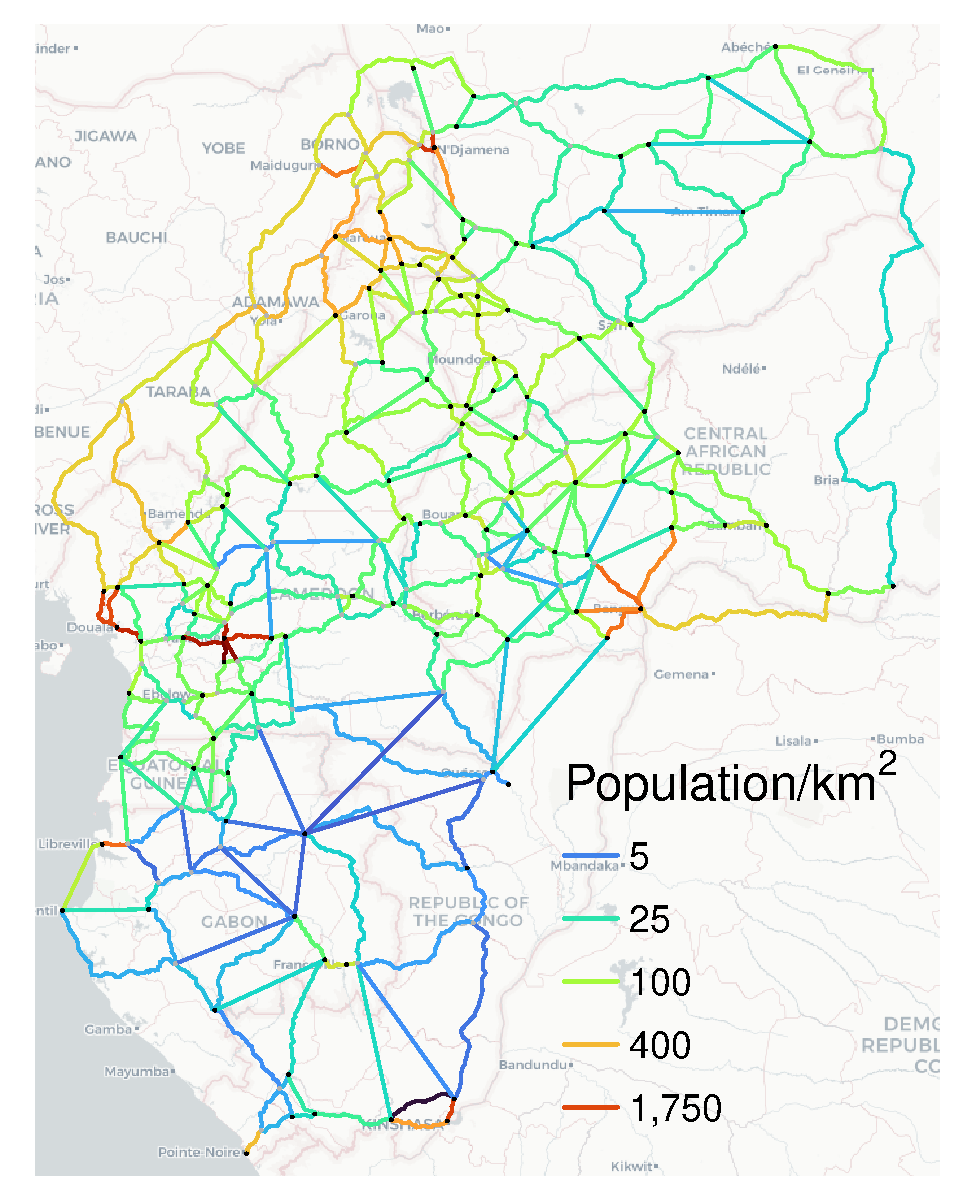
\includegraphics[width=0.38\textwidth, trim= {1cm 0 1cm 0}, clip]{"../figures/trans_CEMAC_network_pop_wpop_km2.pdf"} & 
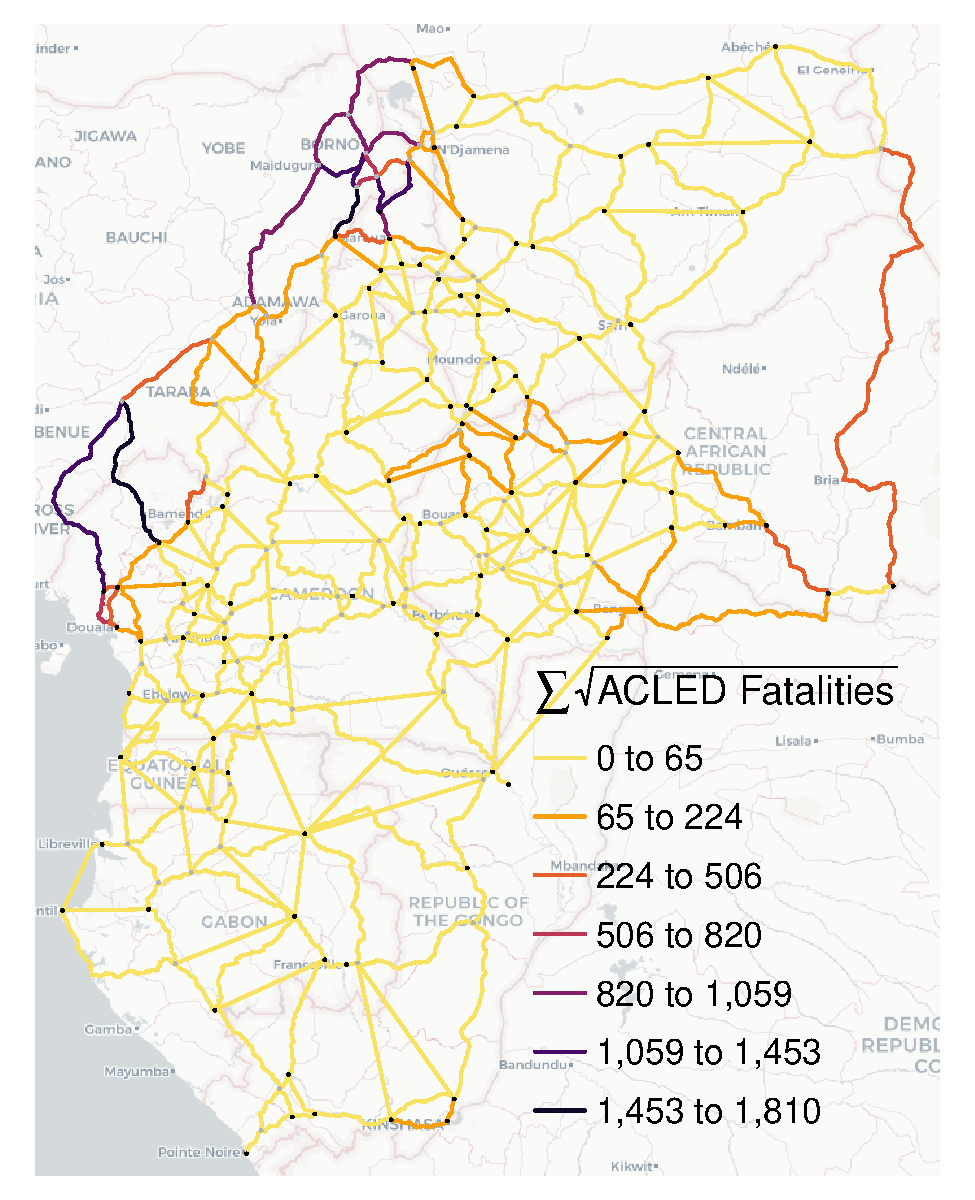
\includegraphics[width=0.38\textwidth, trim= {1cm 0 1cm 0}, clip]{"../figures/trans_CEMAC_network_ACLED_edges_add.pdf"}
\end{tabular}
}
% \raggedright
\scriptsize 
\emph{Notes:} Figure shows average ruggedness and population density within a 3km (two-sided) buffer around links, and $\Omega_j$.
% \vspace{-2mm}
\end{figure}

Figure \ref{fig:RUGG_POP} shows on the LHS ruggedness from \citet{nunn2012ruggedness} and WorldPop 2020 population density; both are estimated within a 3km two-sided buffer around existing and new links. Ostensibly, the area around Bamenda in Cameroon and further north along the Cameroon-Nigeria border is very rugged. This area is also conflict prone $-$ Appendix Figure \ref{fig:ACLED} shows ACLED conflict event data \citep{raleigh2023political} and the RHS of Figure \ref{fig:RUGG_POP} aggregates it around each link following Eq. \ref{eq:conf}. %\citet{collier2016cost}'s road cost prediction model also includes a conflict variable suggesting that costs rise by 20\% during times of violence, but this is not considered in Eq. \ref{eq:COST}. 
Areas around major cities, especially Douala and Yaounde, are highly populated. \newline

Figure \ref{fig:CTW} shows the different types of work and their estimated costs. Total network cost is 27.6 billion USD'15, and all proposed links cost 8 billion USD'15. Total upgrading cost is 19 billion USD'15, of which 0.25 billion is resurfacing, 5.2 billion mixed works, and 13.6 billion upgrades. 

\begin{figure}[H] \vspace{-1mm}
\centering
\caption{\label{fig:CTW} Type of Work and Cost}
\vspace{2mm}
\resizebox{\textwidth}{!}{
\begin{tabular}{@{}c@{}c@{}@{}c@{}} 
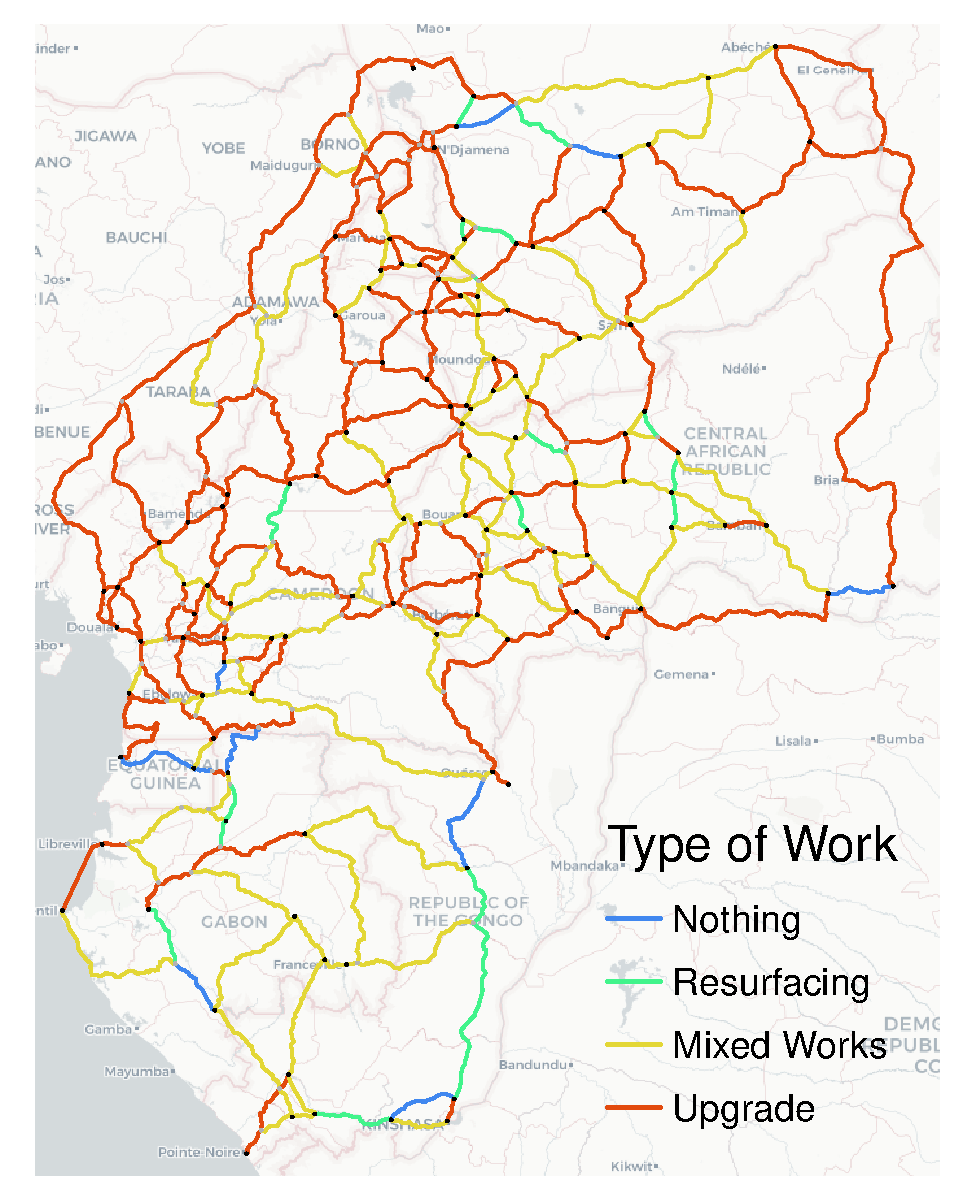
\includegraphics[width=0.38\textwidth, trim= {0.9cm 0 0.9cm 0}, clip]{"../figures/trans_CEMAC_network_type_of_work_google.pdf"} & 
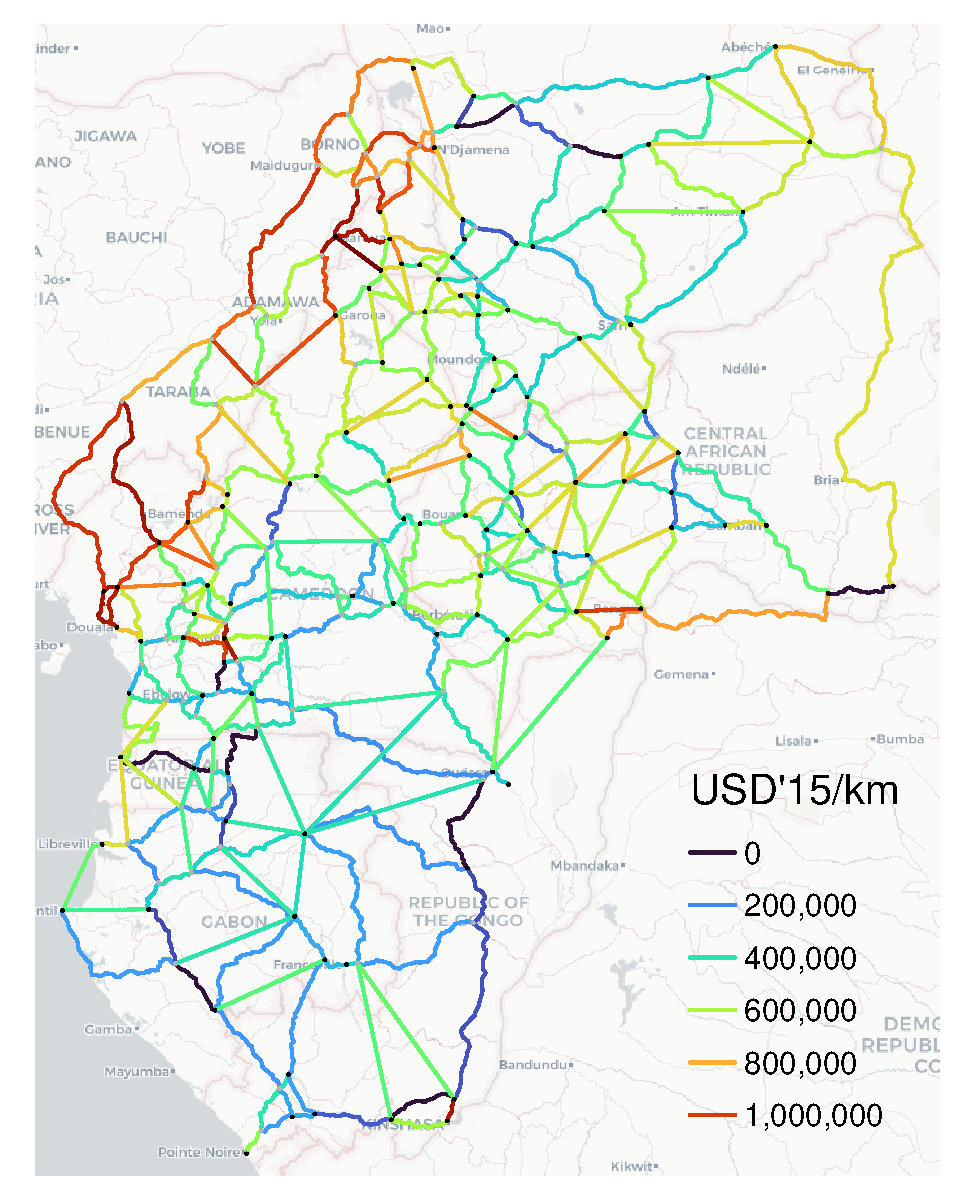
\includegraphics[width=0.38\textwidth, trim= {0.9cm 0 0.9cm 0}, clip]{"../figures/trans_CEMAC_network_all_costs_conflict_google.pdf"} & 
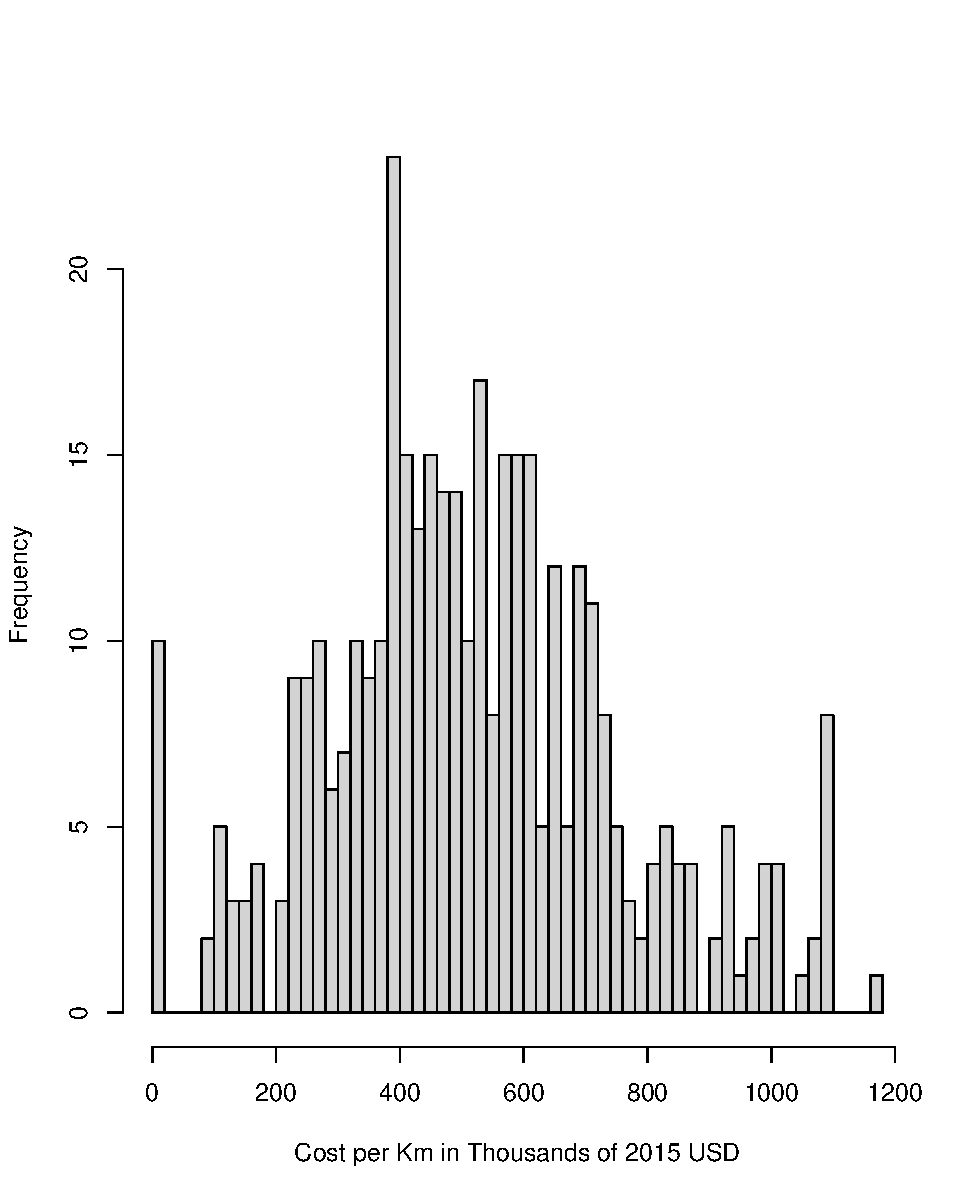
\includegraphics[width=0.38\textwidth, trim= {0.5cm 0 0.5cm 2cm}, clip]{"../figures/trans_CEMAC_network_all_costs_conflict_hist_google.pdf"} 
\end{tabular}
}
% \raggedright
\scriptsize 
\emph{Notes:} Figure shows the type of work and cost depending on link speed: links $<$60km/h need upgrading, between 60 and 80km/h need mixed works, and links 80-90km/h need resurfacing. Links above 90km/h do not need additional work. 
\end{figure}

Following \citet{krantz2024optimal}, I compute link-level cost-benefit ratios as the gain in MA divided by the cost, yielding estimates denominated in \$/min/\$ or 'dollar per minute per dollar invested.' The economic value of such a metric depends on how increases in MA translate into increases in economic activity. \citet{donaldson2016railroads}'s estimates of railroad-induced increases in MA on US land values between 1870 and 1890 suggest that MA translates into economic activity at a rate of 2:1. However, the contemporary African context may be very different. Readers should also note that, particularly in comparison with \citet{krantz2024optimal}, the focus on the CEMAC region alone yields smaller estimates of MA gains from road projects because locations outside of CEMAC which could benefit from them, including traders transiting through CEMAC, are not considered. \newline 

The average gain from upgrading existing links to allows speeds of 90km/h is 0.85\$/min/\$. This drops to 0.47\$/min/\$ under border frictions. In either case, \citet{donaldson2016railroads}'s finding would imply that economic gains are at max half of that; thus, upgrading all links is not sensible. Only 17.5\% of links have gains above 2\$/min/\$ without frictions, indicating medium-term profitability. With frictions only 7.6\% have gains above 2\$/min/\$. \newline 

Figure \ref{fig:MA_PUSD} shows these marginal gains across all links. The yellow and orange links indicate potential medium-term profitability. Notably, except for segments near Yaounde, no proposed link is medium-term profitable under the frictions scenario. However, new links to better connect Equatorial Guinea and Bangui are profitable without frictions. \newline

\begin{figure}[h!]  \vspace{-1mm}
\centering
\caption{\label{fig:MA_PUSD} Investment Returns in \$/min/\$ from Building/Upgrading Each Link to $\geq$90km/h}
\vspace{2mm}
\resizebox{\textwidth}{!}{
\begin{tabular}{@{}c@{}c@{}@{}c@{}} 
No Frictions & 2019 Doing Business Frictions  & Ratio (Frictions/Frictionless) \\
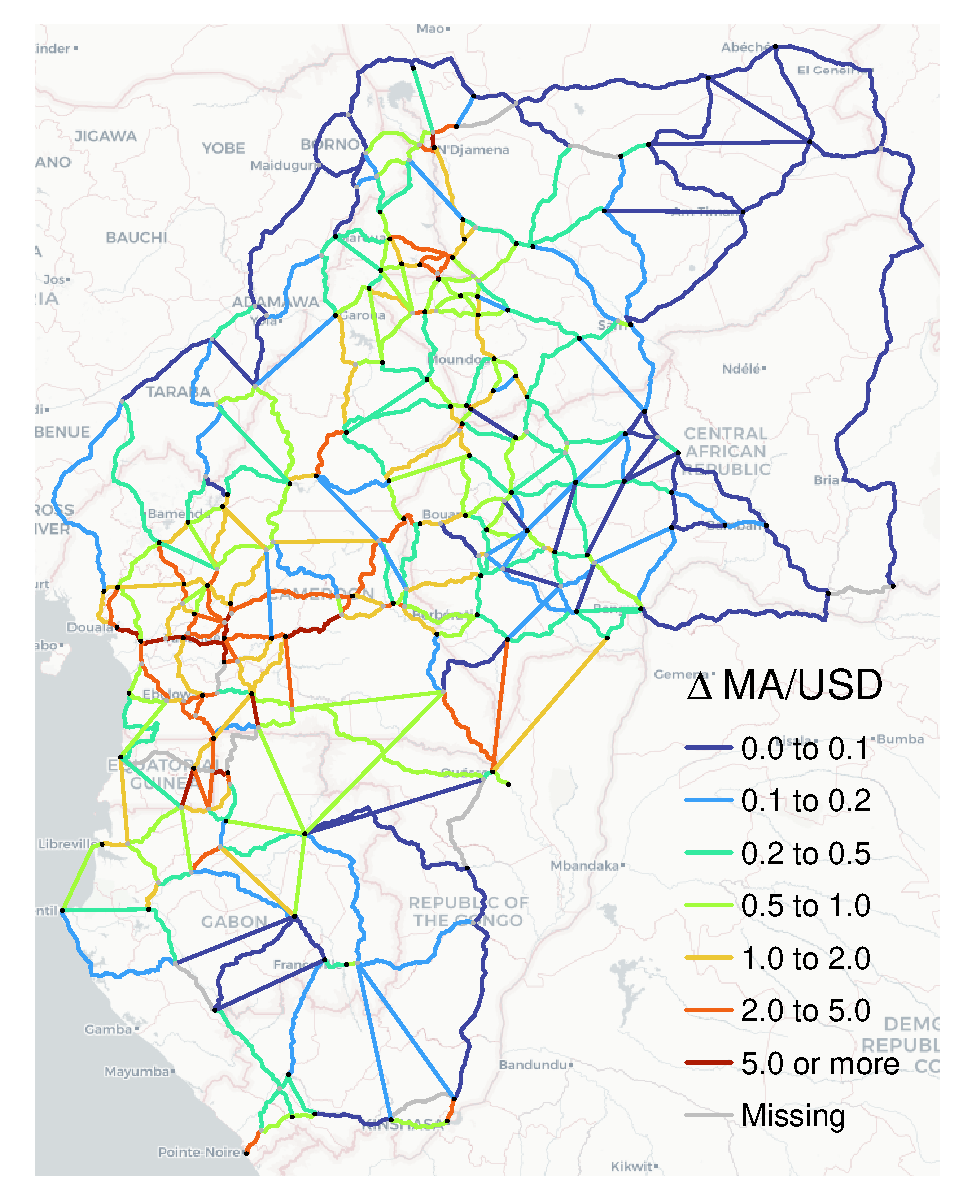
\includegraphics[width=0.38\textwidth, trim= {0.9cm 0 0.9cm 0}, clip]{"../figures/PE/trans_CEMAC_network_MACR_gain_all_90kmh_pusd_google.pdf"} & 
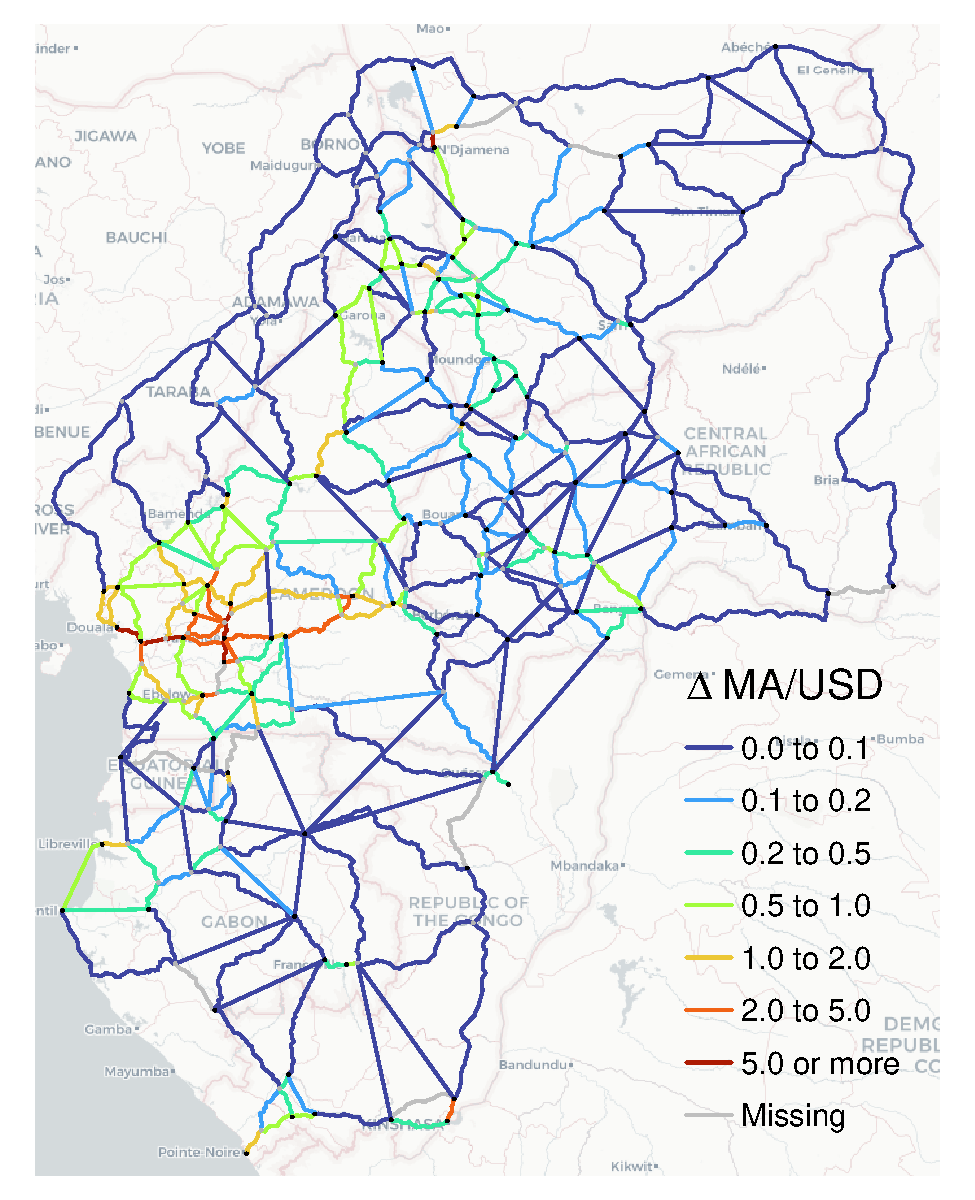
\includegraphics[width=0.38\textwidth, trim= {0.9cm 0 0.9cm 0}, clip]{"../figures/PE/trans_CEMAC_network_MACR_gain_all_90kmh_pusd_bt_google.pdf"} & 
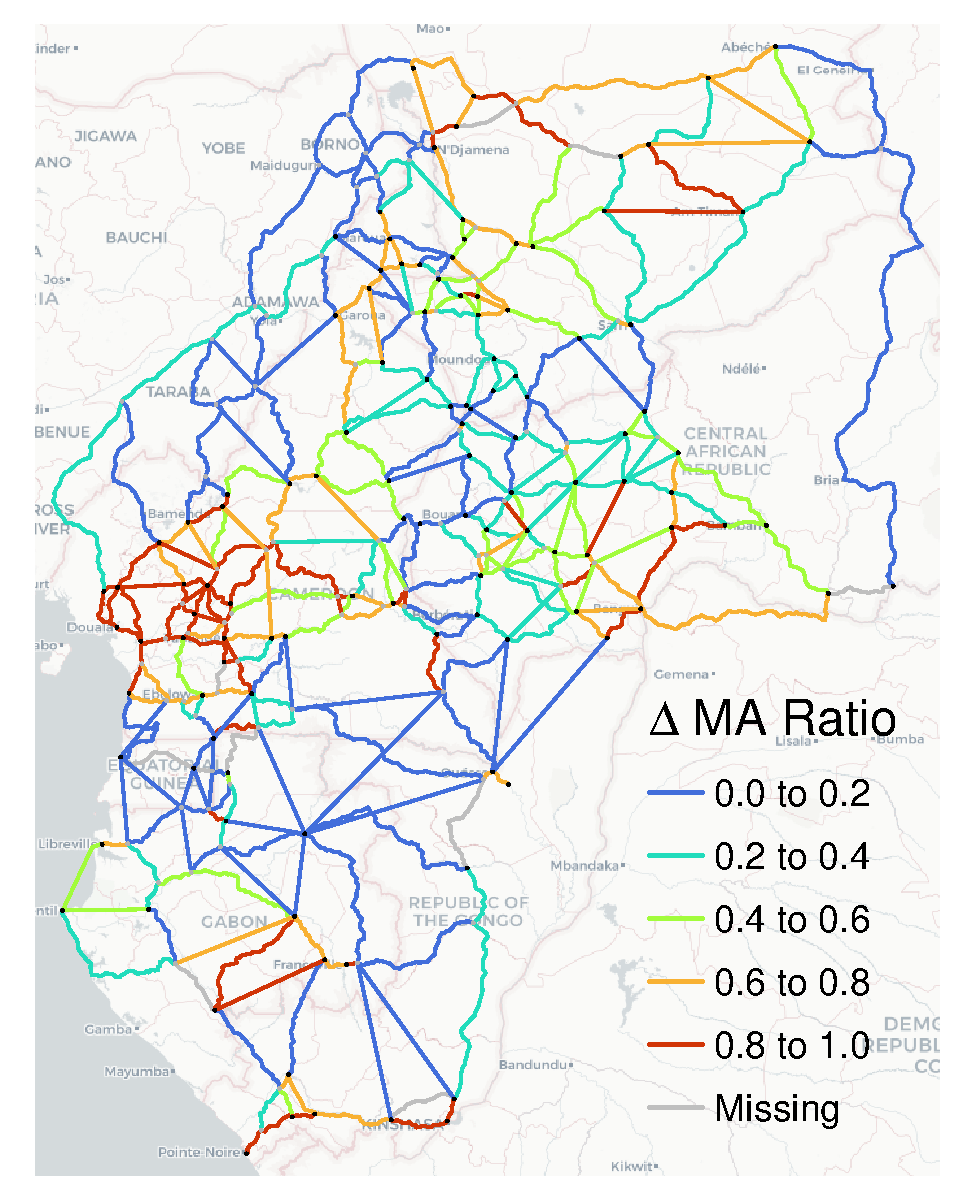
\includegraphics[width=0.38\textwidth, trim= {0.9cm 0 0.9cm 0}, clip]{"../figures/PE/trans_CEMAC_network_MACR_gain_all_90kmh_pusd_bt_ratio_google.pdf"}
\end{tabular}
}
\raggedright
\scriptsize 
\emph{Notes:} Figure shows marginal returns in \$/min/\$ (dollar per minute $=$ MA per dollar invested) from upgrading a link to allow travel speeds of $\geq$90km/h or building a new link. New links, indicated as straight lines, are assumed to be 1.271x longer than their geodesic distance $=$ the inverse of the average route efficiency of 0.787 across existing links in the region.  
 % \vspace{-2mm}
\end{figure}

A good policy is thus to build/upgrade high-yield links along with lesser-yield links for guaranteed positive returns. For example, one could select all links with a marginal return above 0.5\$/min/\$ with or without border frictions, the average return (across frictions/no frictions) of which is shown on the LHS of Figure \ref{fig:UG_cons}. It includes 17.3\% of the length of all existing network and 7.1\% of all proposed link lengths. Building/upgrading these costs 4.25 billion USD'15 and yields a 42.9\% MA gain, amounting to 10.9 billion USD'15/min or 2.56\$/min/\$. Under frictions, the MA gain drops to 7.93 billion USD'15/min or 1.86\$/min/\$. This package may be profitable if we are optimistic about project costs and/or frictions being reduced (or potentially already much lower than in 2019). \newline 

A more prudent package would consider all links with a marginal return above 1\$/min/\$ with or without border frictions, consisting of only the yellow and orange links on the LHS of Figure \ref{fig:UG_cons}. It would cost 2 billion USD'15 and yield a 31.6\% frictionless MA gain, amounting to 8 billion USD'15/min or 4\$/min/\$. Under frictions, the MA gain drops to 6.4 billion USD'15/min or 3.2\$/min/\$, which is still profitable following \citet{donaldson2016railroads}. 

\begin{figure}[H] \vspace{-1mm}
\centering
\caption{\label{fig:UG_cons} Road Packages: High-Yield Links}
\vspace{2mm}
%\begin{tabular}{cc}
%All links $>$0.5\$/min/\$ & All links $>$1\$/min/\$ \\
%% \includegraphics[width=0.48\textwidth]{"../figures/PE/trans_CEMAC_network_MA_gain_100_min_speed_pusd_cons.pdf"} &
%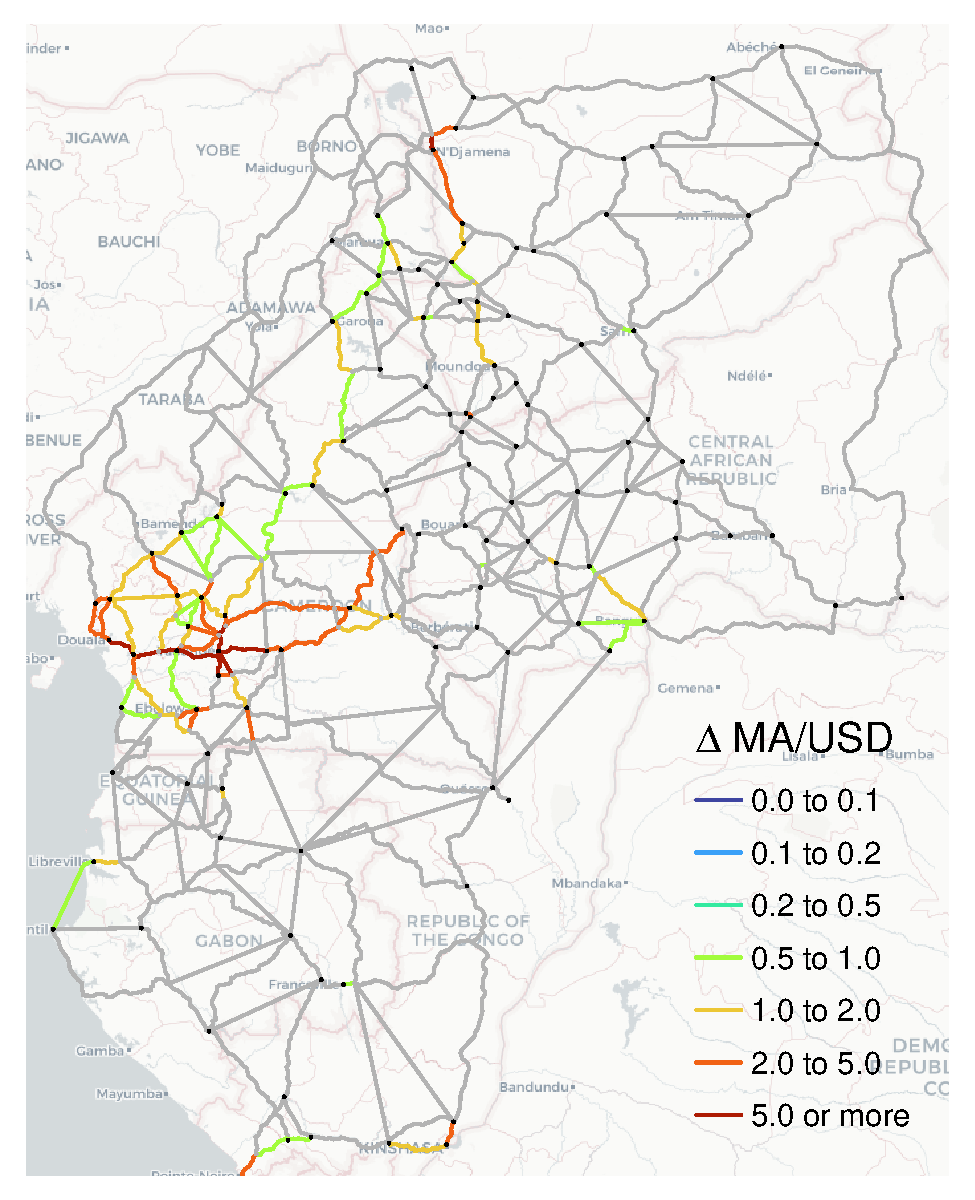
\includegraphics[width=0.48\textwidth]{"../figures/PE/trans_CEMAC_network_MA_gain_all_100kmh_pusd_cons_MAg0.5_google.pdf"} &
%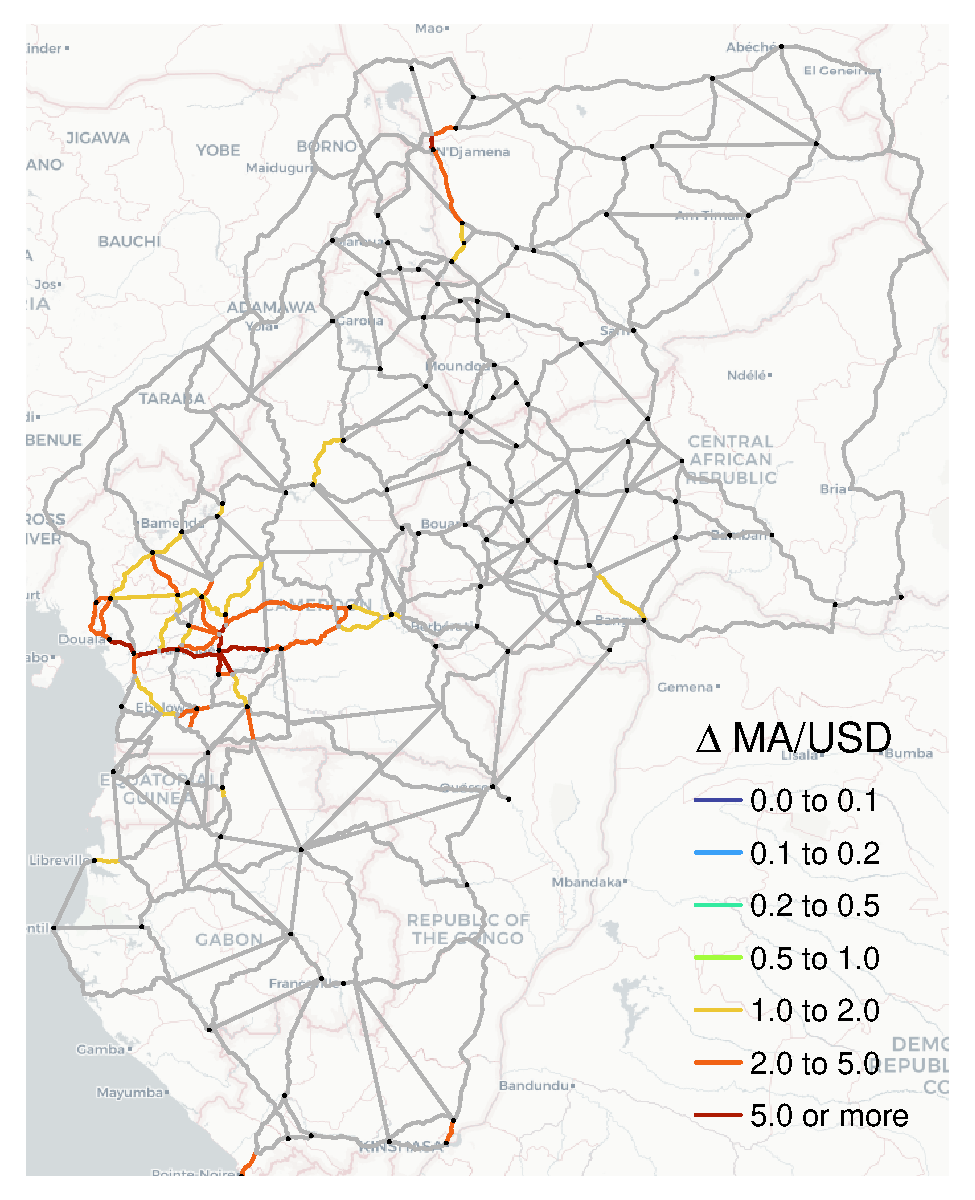
\includegraphics[width=0.48\textwidth]{"../figures/PE/trans_CEMAC_network_MA_gain_all_100kmh_pusd_cons_MAg1_google.pdf"} 
%% \includegraphics[width=0.48\textwidth]{"../figures/trans_CEMAC_network_upgrading_costs.pdf"} \\ [-0.2em]
%\end{tabular}
%% \raggedright
\resizebox{\textwidth}{!}{
\begin{tabular}{@{}c@{}c@{}c@{}} 
Average (FR/NoFR) & No Frictions & NoFR \& NoNewLinks \\
$>\$0.5$ $|$ C: 4.3 $|$ G: 2.6 (43\%) & $>\$1$ $|$ C: 5.4 $|$ G: 2.3 (49\%) & $>\$1$ $|$ C: 4 $|$ G: 2.8 (44\%) \\
Frictions G: 1.9\$/min/\$ (53\%) & Frictions G: 1.4\$/min/\$ (51\%) & Frictions G: 1.7\$/min/\$ (47\%) \\ [-0.5em]
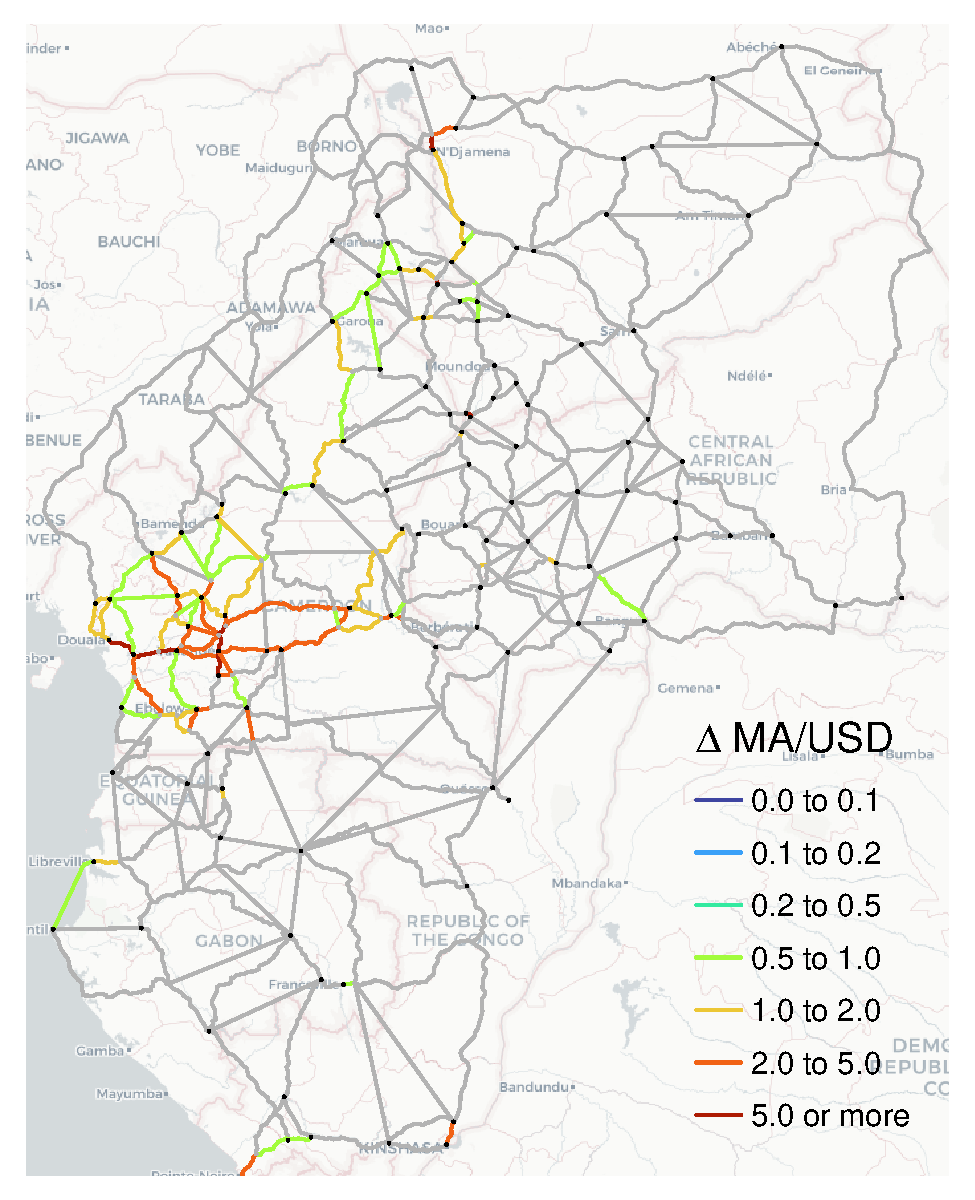
\includegraphics[width=0.38\textwidth, trim= {0.9cm 0 0.9cm 0}, clip]{"../figures/PE/trans_CEMAC_network_MACR_gain_all_90kmh_pusd_cons_MAg0.5_google.pdf"} & 
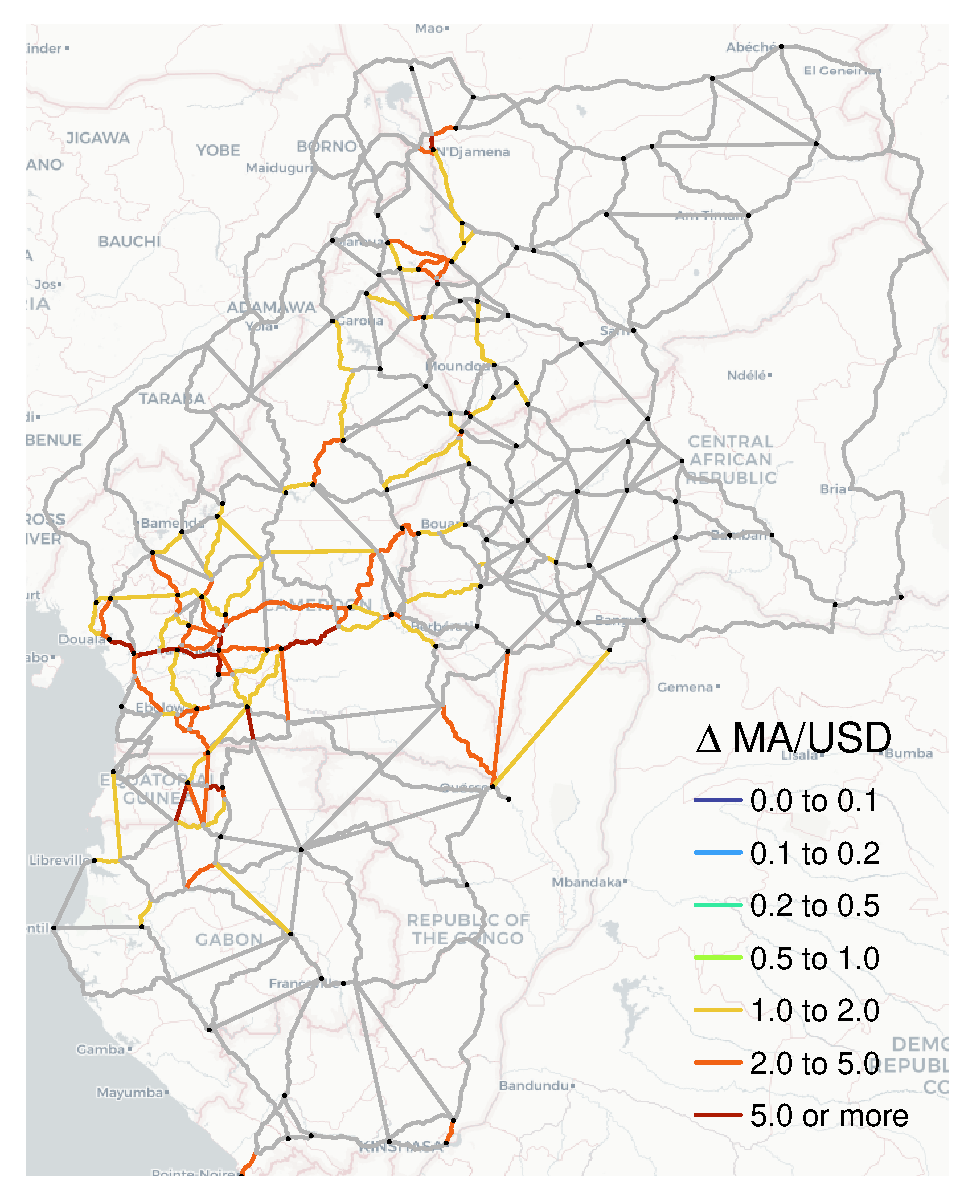
\includegraphics[width=0.38\textwidth, trim= {0.9cm 0 0.9cm 0}, clip]{"../figures/PE/trans_CEMAC_network_MACR_gain_all_90kmh_pusd_cons_nofr_MAg1_google.pdf"} &
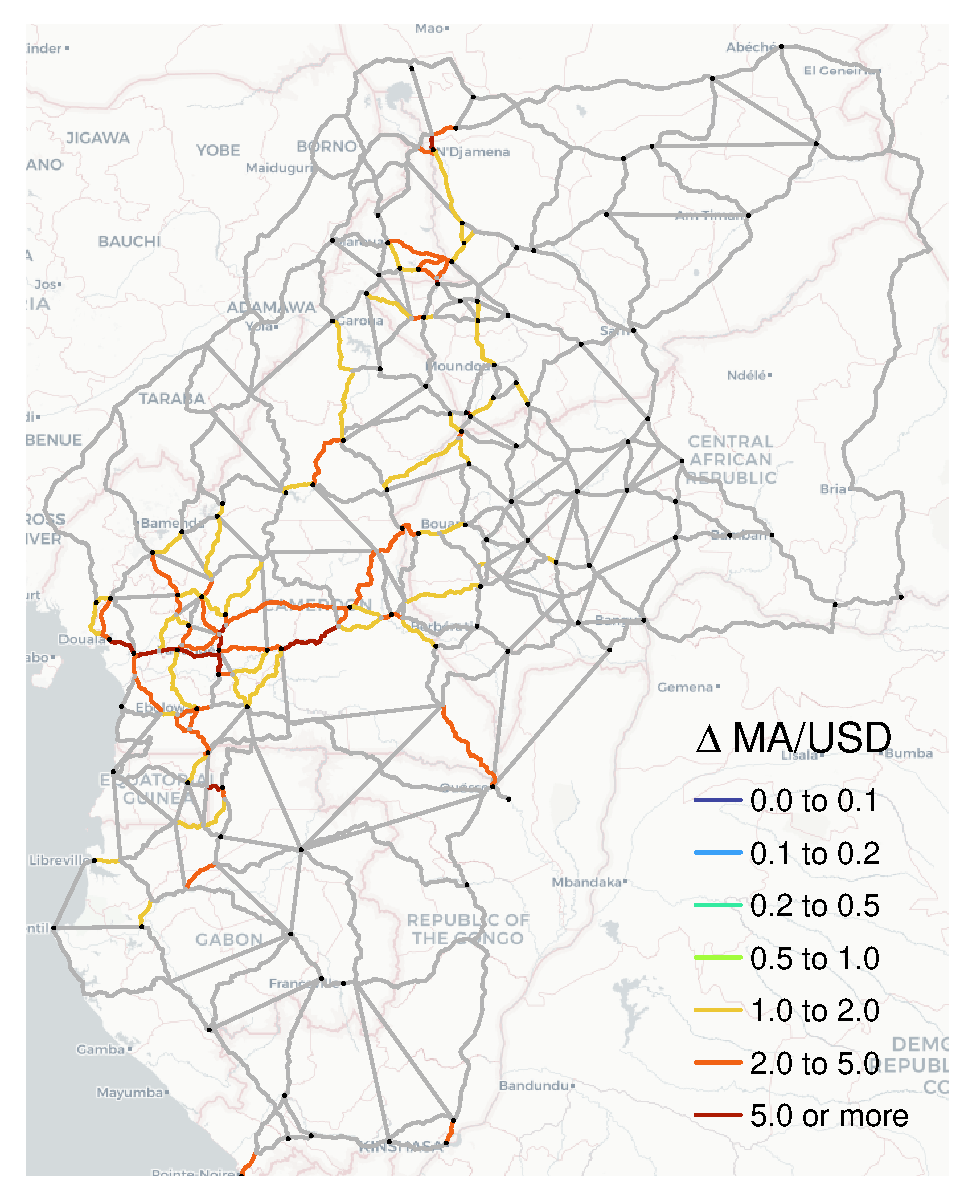
\includegraphics[width=0.38\textwidth, trim= {0.9cm 0 0.9cm 0}, clip]{"../figures/PE/trans_CEMAC_network_MACR_gain_all_90kmh_pusd_cons_nofr_noadd_MAg1_google.pdf"}  
\end{tabular}
}
\scriptsize 
\emph{Notes:} Figure shows the average marginal returns to building/upgrading selected links across the frictions and no frictions scenarios. LHS: links have marginal gains above the threshold value with and without border frictions.  
\end{figure}

We could also be more optimistic and assume that border frictions will be strongly reduced or eliminated in the foreseeable future and thus focus on optimal links in the absence of frictions. The middle panel of Figure \ref{fig:UG_cons} shows all links with a marginal return above 1\$/min/\$ without border frictions. This package contains 20\% of all existing and proposed links, would cost 5.4 billion USD'15, and yield a 49\% frictionless MA gain, amounting to 12.5 billion USD'15/min or 2.3\$/min/\$. Under frictions, the MA gain would drop to 7.6 billion USD'15/min or 1.4\$/min/\$, which is unprofitable following \citet{donaldson2016railroads}. \newline

 % This package may be profitable if we are optimistic about frictions being reduced, or potentially already much lower than in 2019.
% yields a joint MA gain (after recalculating all shortest paths) of 12.9\% without frictions, amounting to \$3.91 billion or 4.25\$/min/\$. Under border frictions, the MA gain drops to \$2.97 billion or 3.22\$/min/\$. 

Since building expensive new links lowers the returns to this package and may not be the policymakers' intention, I also consider the same package without new links on the RHS of Figure \ref{fig:UG_cons}. It then would cost only 4 billion USD'15 and yield a 44\% frictionless MA gain, amounting to 11.2 billion USD'15/min or 2.8\$/min/\$. Under frictions, the MA gain would drop to 7 billion USD'15/min or 1.7\$/min/\$. \newline 

More accurate information about border frictions and economic returns to MA in the region would be beneficial for making a good assessment. MA maximization is also not a redistributional policy, but planners may have legitimate redistributional objectives and explicit budget constraints. The condition of roads and their upgrading costs may also not be accurately captured by routing engines and calibrated remote sensing estimates following \citet{collier2016cost} and \citet{fajgelbaum2020optimal}. Thus, knowledge of the region, its road network, and engineering constraints must also be considered. \newline 

A final assessment regards macroeconomic feasibility in present-discounted-value (PDV) terms. Here, I also follow \citet{krantz2024optimal} and consider the minimum increase in the macroeconomic growth rate from each package necessary to break even after 30 years, discounting the future by 10\%. As mentioned, CEMAC's GDP in 2023 was 90.1 billion in 2015 USD. Its growth rate between 2003 and 2023 was 3.5\% on average, and the IMF projects a growth of 3.8\% from 2024-2029. Thus, I take a 3.5\% baseline growth rate as the realistic scenario, but also simulate a 2\% growth rate as a pessimistic scenario. Table \ref{tab:MACAB} reports the increases in the macroeconomic growth rate of the region necessary for road projects to break even after 30 years. 
% For interpretation details see \citet{krantz2024optimal} Table 7 ff. % However, as discussed in \citet{krantz2024optimal}, under debt financing and significantly higher project costs positive macroeconomic returns may not accrue anymore for the lower yield packages.  

\begin{table}[H] \vspace{-2mm}
\centering
\caption{\label{tab:MACAB} Break Even Changes in the Macroeconomic Growth Rate for Different Investments}
\vspace{2mm}
\begin{tabular}{lrrrr} \toprule
\textbf{Work Package} & \textbf{Cost} & \textbf{\%$\Delta$MA} & \textbf{BEG} (3.5\%) & \textbf{BEG} (2\%) \\ \midrule
% Full Extension ($\uparrow$RE) & \$56.1B & $3.9-\hphantom{5}5.5$ & 0.31\% $\to$ 4.113 & 0.50\% $\to$ 3.015 \\
% Consensus Extension ($\uparrow$RE) & \$12.1B & $2.4-\hphantom{5}4.0$ & 0.07\% $\to$ 4.103 & 0.11\% $\to$ 3.003 \\
% Full Upgrade ($\uparrow$TE) & \$105.7B  & $27.0-42.1$ &  0.58\% $\to$ 4.124 & 0.94\% $\to$ 3.028 \\
% Consensus Upgrade ($\uparrow$TE) & \$45.0B  & $21.2-33.1$ &  0.25\% $\to$ 4.110 & 0.40\% $\to$ 3.012 \\
All Works & \$27B  & $68-72$ &  5.79\% $\to$ 3.703 & 12.7\% $\to$ 2.253 \\
All Upgrades & \$19B  & $60-64$ &  4.10\% $\to$ 3.643 & 8.96\% $\to$ 2.179 \\
Links $>\$0.5$/min/\$ (Avg) & \$4.3B & $43-53$ & 0.94\% $\to$ 3.533 & 2.05\% $\to$ 2.041 \\
Links $>\$1$/min/\$ (NoFR) & \$5.4B & $49-51$ & 1.17\% $\to$ 3.541 & 2.57\% $\to$ 2.051 \\
All Links $>\$1$/min/\$ (NFNN) & \$4B & $44-47$ & 0.87\% $\to$ 3.530 & 1.91\% $\to$ 2.038 \\
   \bottomrule  \\ [-0.9em]
\multicolumn{5}{l}{\parbox{0.9\textwidth}{\footnotesize
\textit{Notes:} Table shows the cost in 2015 USD PPP of different investment packages, their MA \%-gain under frictions (LHS) and frictionless (RHS) scenarios, and the change in CEMAC's macroeconomic growth rate needed to break even after 30 years under realistic (3.5\%) and pessimistic (2\%) baseline growth. }}
\end{tabular}
\end{table} 

Ostensibly, in all three investment packages, the ratio of the change in MA to the break-even change in the macroeconomic growth rate is greater than 40, suggesting that these packages should all be macroeconomically feasible in the medium run under mild assumptions about the economic returns to increased market access. For example, the package with all links $>0.5$\$/min/\$ returns with and without frictions costs \$4.3B USD'15 and yields a 43-54\% MA gain. Under the 3.5\% baseline growth scenario, the investment would need to raise the macroeconomic growth rate by around 1\% to 3.533\% for the investment to break even after 30 years. This implies \%$\Delta$MA$\to$\%$\Delta$\%$\Delta$GDP of 40:1, which is much smaller than the 2:1 estimated by \citet{donaldson2016railroads} as the historical US the land price-elasticity to MA over 20 years. \newline 

However, long-run changes in the growth rate may be difficult to sustain. Elasticities also have the major drawback of being scale-independent. In this particular case, the percentage change in MA from the investment is 53\% under frictions versus 43\% in the frictionless case. In contrast, the MA gain is only \$7.93B/min under frictions vs. \$10.9B/min in the frictionless case. \newline 

The main takeaway from this exercise should thus be that only relatively small changes ($\sim$1\%) in the region's macroeconomic growth rate are needed to finance these packages in the medium run (30 years). It appears plausible that the sizeable MA gains could induce such changes, but we know little about economic returns to MA and even less relating it to long-term growth.  




\newpage


\section{Optimal Network Investments in General Equilibrium}

The General Equilibrium simulations also closely follow \citet{krantz2024optimal}, utilizing the quantitative framework of \citet{fajgelbaum2020optimal} and some parameters taken from \citet{graff2024spatial}.\footnote{In particular the consumption share in utility ($\alpha = 0.7$), elasticity of substitution between different consumption goods ($\sigma = 3.8$), congestion parameter ($\beta = 1.177$), and returns to infrastructure ($\gamma = 0.946$) in the standard decreasing returns case and $\gamma^* = \beta^2/\gamma = 1.464$ in the increasing returns case.} As in \citet{krantz2024optimal}, I let ports produce the imports. Since the region also has land borders, I apply the same scaling factor to the ports' export volume in 2020 Q1, which is obtained considering imports and ports of the entire continent. This yields that imports through the region's 6 ports are 16.9\% of the region's GDP. The total imports of goods and services in the region from 2019-2023 was 28.2\% of GDP, and the merchandise imports were 19.2\% of GDP, so this assumes that the bulk of merchandise imports came in through the region's 6 international ports.  

\begin{figure}[H] \vspace{-1mm}
\centering
\caption{\label{fig:Graph_Calib} Calibrated Network for General Equilibrium Simulations}
\vspace{2mm}
\resizebox{\textwidth}{!}{
\begin{tabular}{@{}c@{}c@{}@{}c@{}} 
Nodes by Type & Speed + IWI + Outflows & Calibration: Total Productivity \\
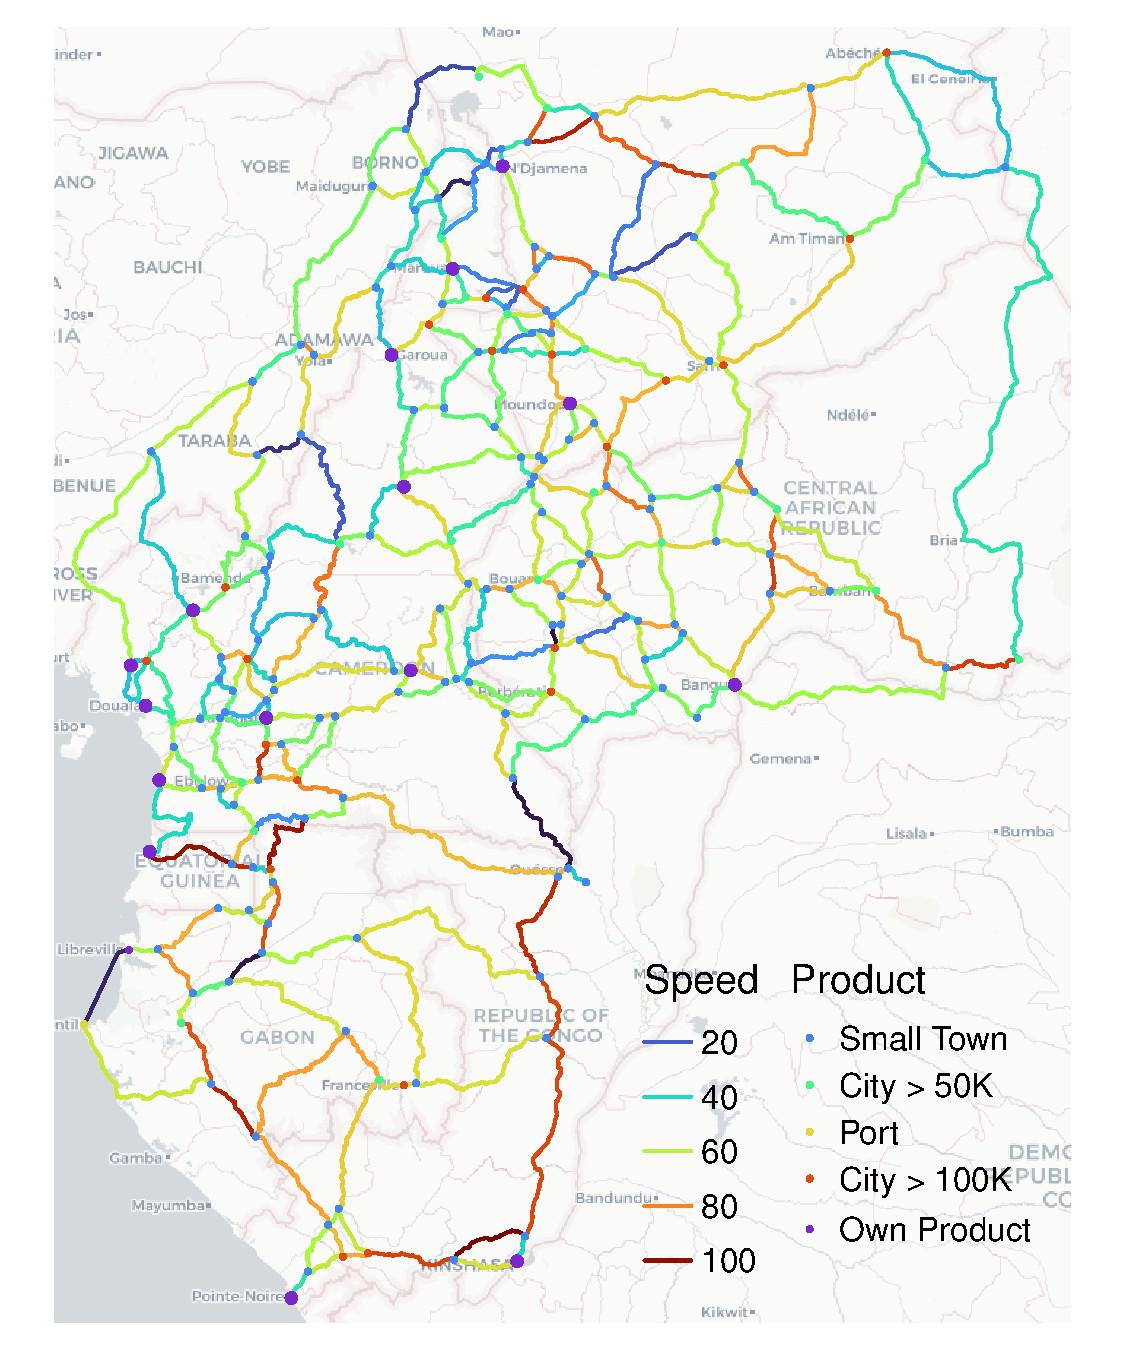
\includegraphics[width=0.38\textwidth, trim= {1.1cm 0 1.2cm 0}, clip]{"../figures/GE/trans_africa_network_reduced_20_products_google.pdf"} & 
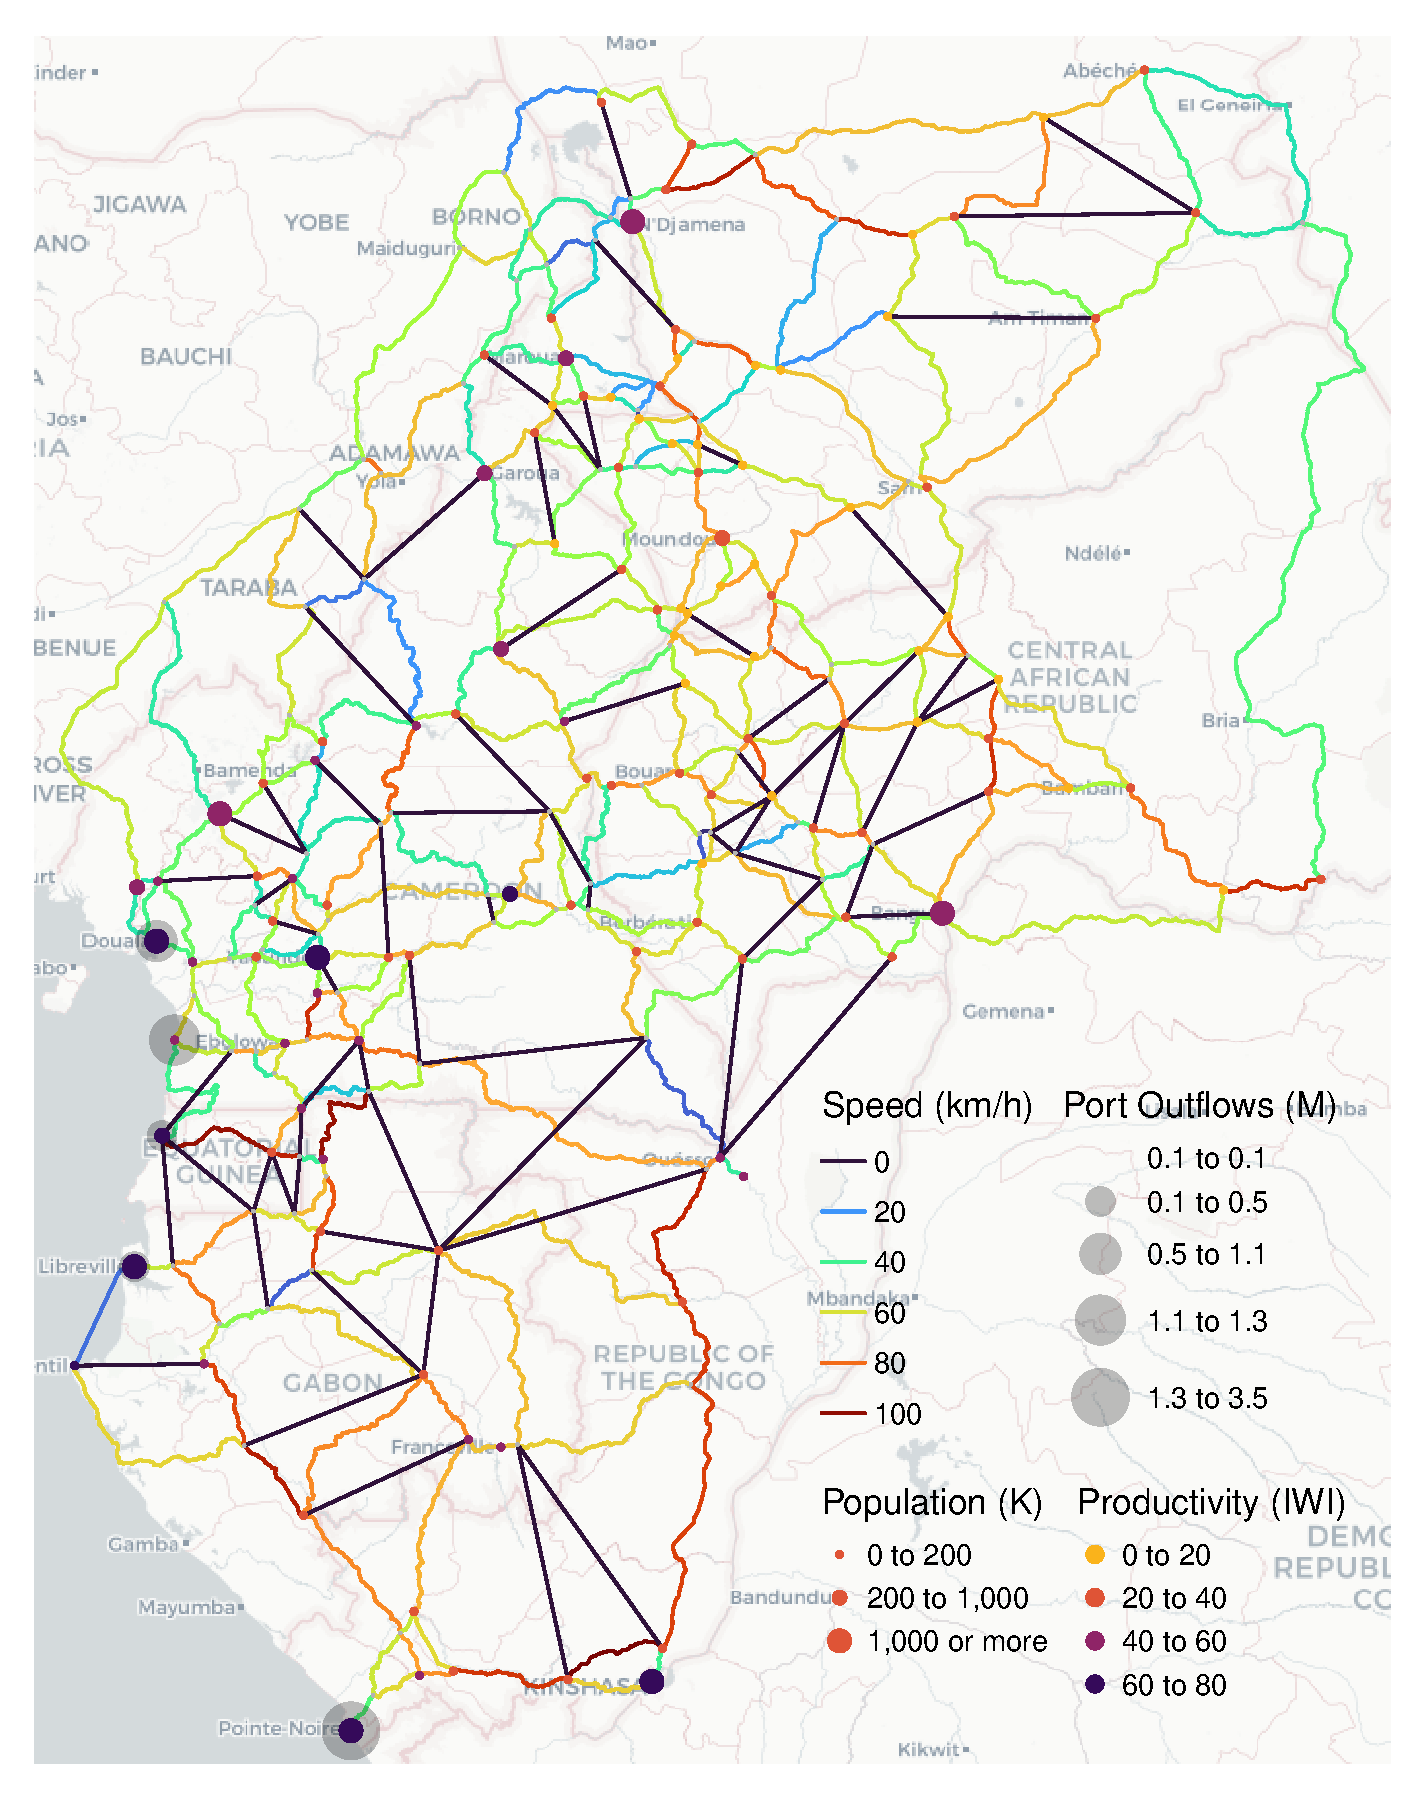
\includegraphics[width=0.38\textwidth, trim= {0.9cm 0 0.9cm 0}, clip]{"../figures/trans_CEMAC_network_GE_parameterization_latest_google.pdf"} & 
\includegraphics[width=0.38\textwidth, trim= {0.9cm 0 0.9cm 0}, clip]{"../figures/trans_CEMAC_network_GE_parameterization_latest_MACR_90kmh_google.pdf"}
\end{tabular}
}
\raggedright
\scriptsize 
\emph{Notes:} Figure shows network calibrated with speed, city population and productivity and port outflows. The middle panel shows the IWI, which is multiplied by population to distribute 80\% of the region's GDP and thus makes up the bulk of the productivity measure. Total productivity, shown on the RHS and obtained as GDP divided by population, additionally considers crop production (20\% of GDP). It is highest in some small cities, which are agricultural hubs. Port outflows are translated following \citep{krantz2024optimal} into intnl. productivity to produce imports amounting to 16.9\% of GDP. 
% \vspace{-10cm}
\end{figure}

To create incentives for trade through the network, I let 16 cities with a population of $>$200,000 or ports with outflows of $>$1M TEU in 2020 Q1 produce their own product. The remaining cities are classified into port (positive outflows), large city with population $>$ 100,000, medium-sized city with population $>$50,000, and town/unpopulated node otherwise. The nodes are parameterized with total productivity ($=$ GDP/population) and population. Port cities have additional international productivity to produce 16.9\% of GDP worth of imports.\footnote{Amounting to $(\text{outflows [TEU] in 2020 Q1}\times 2100)/\text{population}$, where the factor of 2100 is a translation of the factor of 37 from \citet{krantz2024optimal} based on the IWI to the GDP scale.} Edges are parameterized with speed in km/h; infrastructure building cost, iceberg trade cost, and (optionally) border frictions, exactly following \citet{krantz2024optimal} except for Eq. \ref{eq:COST}. Figure \ref{fig:Graph_Calib} shows the classified and parameterized graph. \newline 


I set the elasticity of substitution equal to $\sigma = 3.8$ following \citet{bajzik2020estimating} and \citet{armington1969theory} because this setting resembles products differentiated by origin traded in an international context. I simulate cases with ($\rho = 2$) or without ($\rho = 0$) inequality aversion and border frictions, as well as with or without new links, for planning budgets of 1, 2, and 4 billion USD'15, which is about 1.19, 2.38, and 4.76 billion in current USD, respectively. I also consider the case of increasing returns to infrastructure ($\gamma^* > \beta$, default is $\gamma < \beta$) with $\gamma^* = \beta^2/\gamma$, i.e., inverting the ratio of $\beta$ (congestion) and $\gamma$ (returns to infrastructure) parameters keeping $\beta$ fixed as in \citet{fajgelbaum2020optimal}. The Appendix also reports results for a 5 billion budget. As mentioned, upgrading all links to $\geq$90km/h would cost 19 billion USD'15, and constructing all proposed links would cost 8 billion USD'15. I start with scenarios where planners can only upgrade existing links. 

\subsection{Upgrading Roads} 

Figure \ref{fig:GE_UGNOfr} shows the results, in terms of the fraction of the link upgraded, from planners optimally spending 1, 2, or 4 billion on upgrading the network without frictions. Clearly, these planners focus on better connecting the central populated regions, particularly in central Cameroon and at the Cameroon-Chad border area. But also the roads between Point-Noire and Brazzaville and between Bangui and Mbaiki and from Ouesso into Cameroon are upgraded. \newline %All planners also upgrade the slow ferry connection between Libreville and Port-Gentil, implying that building a road connecting the two has high priority. 

With inequality aversion, planners spend a bit more in poorer northern Chad and less in the richer coastal regions. Since with upgrading the network structure is fixed, increasing returns (IRS) only has minor impact on the optimal allocation. More notable is that the generated trade flows (visualized for selected cities and the \$2B budget case in Appendix Figure \ref{fig:GE_UGNOfrFL}) and also the total welfare gain (WG) is significantly higher in the IRS case. This is because in \citet{fajgelbaum2020optimal}'s model equilibrium trade flows of good $n$ are $Q^n_{jk} = I_{jk}^\frac{\gamma}{\beta}\Psi^n_{jk}$, where $\Psi^n_{jk}$ is a function of parameters and prices. Higher flows imply a more diverse CES consumption basket, giving higher utility, and a larger $\gamma$ (larger $\gamma/\beta$ ratio) implies greater sensitivity to changes in $I_{jk}$. \newline 

 Thus, precisely estimating the transport parameters $\beta$ and $\gamma$ as well as the elasticity of substitution $\sigma$ would be necessary for accurate welfare assessments (reported gains need to be treated with caution). Fortunately, except for lowering $\sigma$ a lot, infrastructure allocations are not very sensitive to these parameters. Yet, it is notable that inequality aversion ($\rho = 2$) yields slightly lower aggregate welfare gains (e.g., of 0.9\% instead of 1\% in the \$4B investment case) in favour of a more equitable distribution of gains.  \newline 

I also run the simulations with border frictions. Figure \ref{fig:GE_UGFR} reports the difference to the frictionless case. As in \citet{krantz2024optimal}, frictions lead to slight alterations in the optimal allocation away from expensive border-crossing links. In some cases, other border-crossing links are strengthened instead, and funds are directed to building more domestic links. Overall, the effects of frictions are minor, presumably because they enter iceberg trade costs through a log function (see \citet{krantz2024optimal} Eq. 12), and non-trivial as the resulting reallocations are a complex GE outcome. \newline 

Appendix Figure \ref{fig:GE_UGNOfr_5b} shows the optimal 5 billion spending. The side-by-side view and large budget allow a better examination of the minor differences between the three planners. Overall, the inequality-averse planner upgrades slightly more roads in the poorer north (Chad, CAR), whereas the IRS planner concentrates investments on fewer links and is thus able to partly upgrade a passage through Nigeria. Frictions reduce cross-border spending, especially across the Cameroon-Chad and Cameroon-CAR borders, but also at the border to Equatorial Guinea. 
% Here the planner upgrades two full corridors from Cameroon up north via Bertoua and Ngaoundere, respectively, and also the full road between Point-Noire and Brazzaville. Under inequality aversion, also the road between Bangui and N'Djamena is updated, alongside many roads connecting cities near the Cameroon-Chad border.  

\subsection{Building and Upgrading Roads} 

When planners also have the ability to build new roads alongside upgrading existing ones, they almost exclusively choose to do so under standard decreasing returns assumption ($\gamma < \beta$: congestion forces are strong), despite such links being more expensive. This stands in contrast to results for the entire African network \citep{krantz2024optimal}, where planners invest $\sim$70\% in upgrading even under decreasing returns, indicating that particularly in the CEMAC region, much can be gained by increasing the network route efficiency through new roads. Figure \ref{fig:GE_BUGNOfr} shows the results, with overall very similar allocations for the standard and inequality-averse planners; the share of new roads decreases from 93\% with the \$1B budget to 73\% under the \$4B budget. \newline 

The bottom panel of Figure \ref{fig:GE_BUGNOfr} shows allocations of the increasing returns planner ($\gamma > \beta$: congestion forces are weak), yielding reversed relative allocations between building and upgrading road: IRS planners at all budgets spend more than 95\% on upgrading. The only links that are built are the ferry connection between Libreville and Port-Gentil, which is turned into a road, and, under the \$4B budget, a new road between Libreville (Kougouleu) and Bata in Equatorial Guinea. \newline

Border frictions, shown in the bottom panel of Figure \ref{fig:GE_BUGFR}, again reduce investment in certain border-crossing links in favour of others and domestic links. The most notable change is under the IRS \$4B planner, which does not build the expensive border-crossing new road from Libreville (Kougouleu) to Bata under frictions but instead strengthens other parts of the network. 


\begin{figure}[H] \vspace{-5mm}
\centering
\caption{\label{fig:GE_UGNOfr} Welfare Maximizing Infrastructure Spending in GE: Upgrading Links}
\vspace{2mm}
\resizebox{\textwidth}{!}{
\begin{tabular}{@{}c@{}c@{}c@{}} 
\$1B USD'15 $|$ WG: 0.4\% & \$2B USD'15 $|$ WG: 0.6\% & \$4B USD'15 $|$ WG: 1\%  \\
Upgraded: 1529km & Upgraded: 3103km & Upgraded: 6844km \\ 
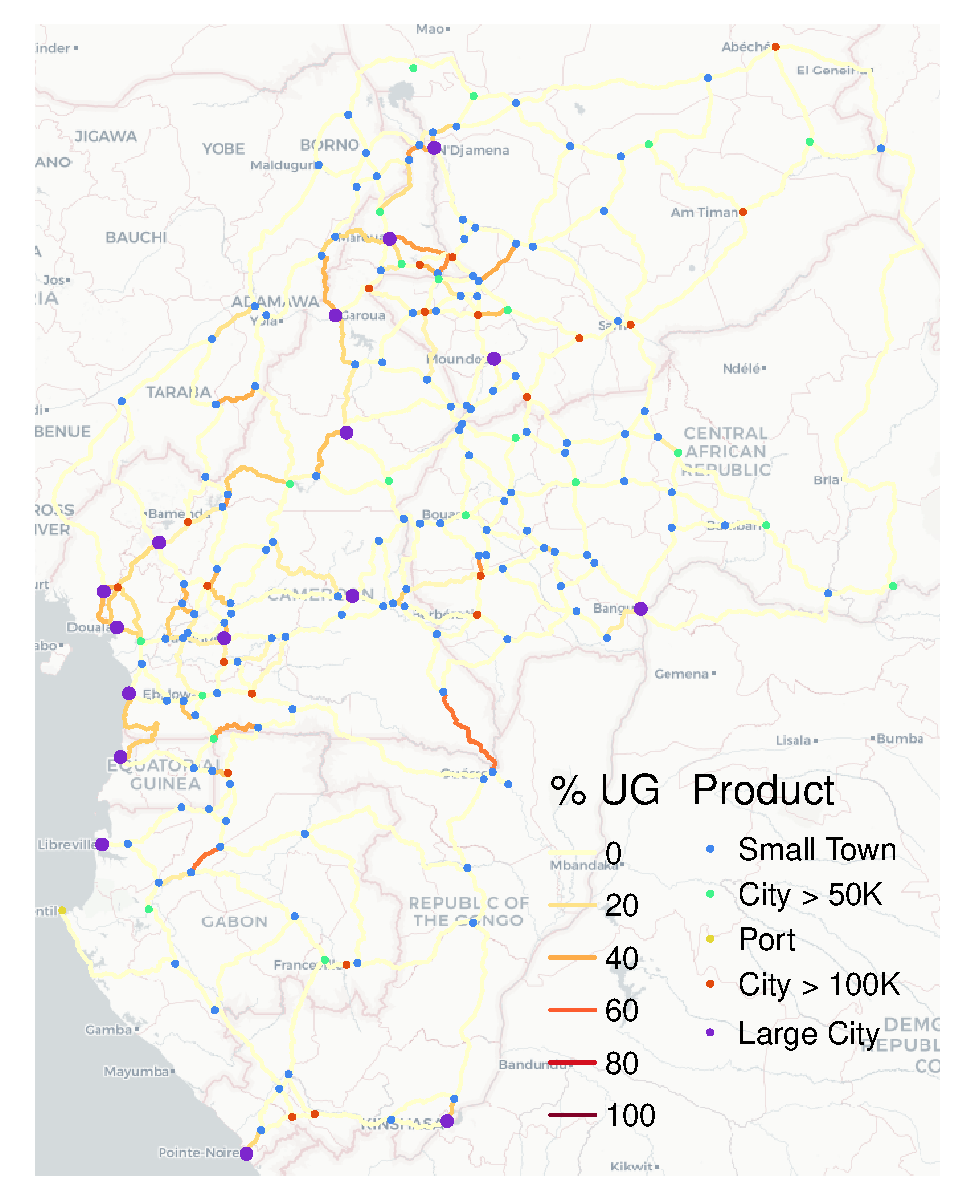
\includegraphics[width=0.38\textwidth, trim= {0.9cm 0 0.9cm 0}, clip]{"../figures/GE/trans_africa_network_GE_20g_1b_fixed_cgc_sigma3.8_rho0_julia_MACR_90kmh_google_perc_ug.pdf"} & 
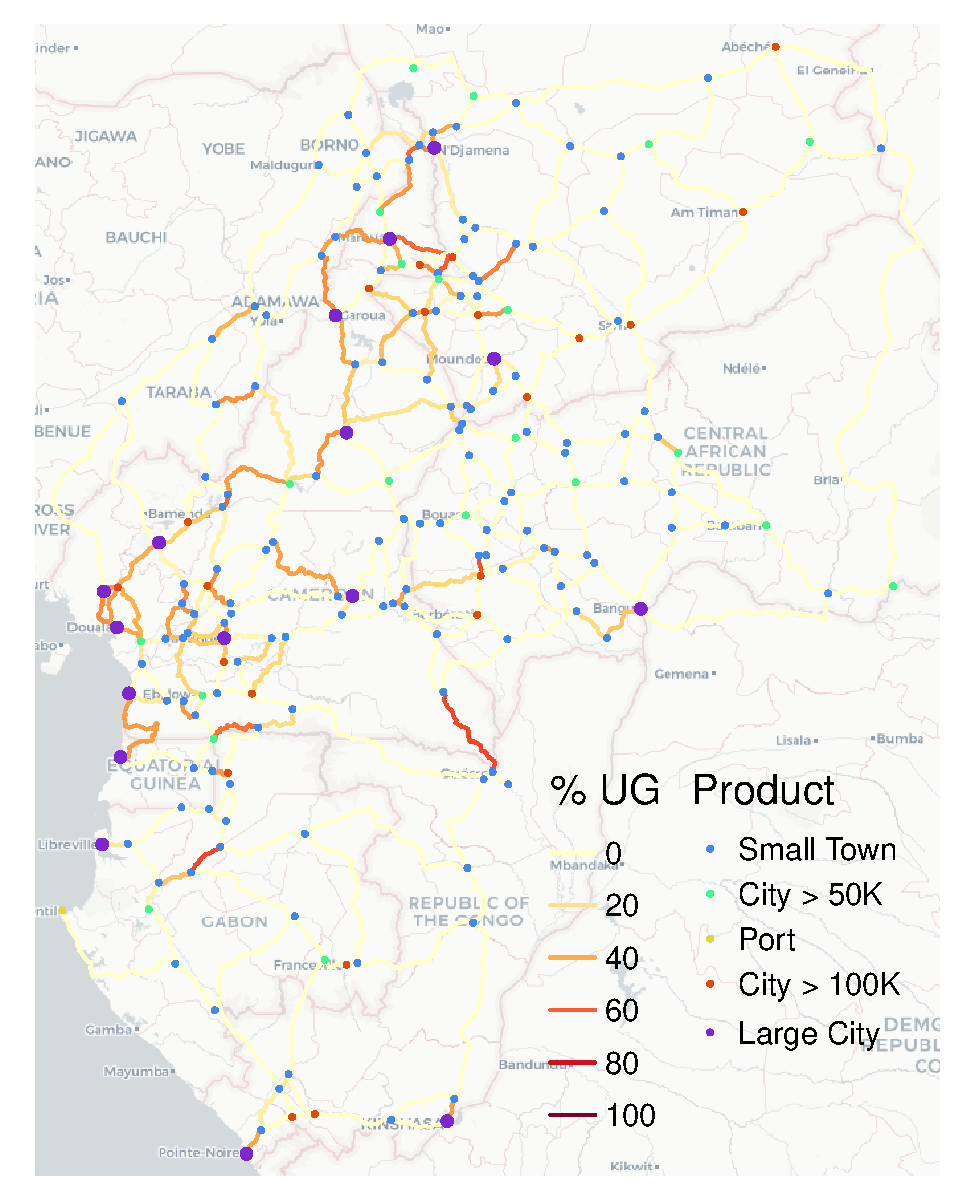
\includegraphics[width=0.38\textwidth, trim= {0.9cm 0 0.9cm 0}, clip]{"../figures/GE/trans_africa_network_GE_20g_2b_fixed_cgc_sigma3.8_rho0_julia_MACR_90kmh_google_perc_ug.pdf"} &
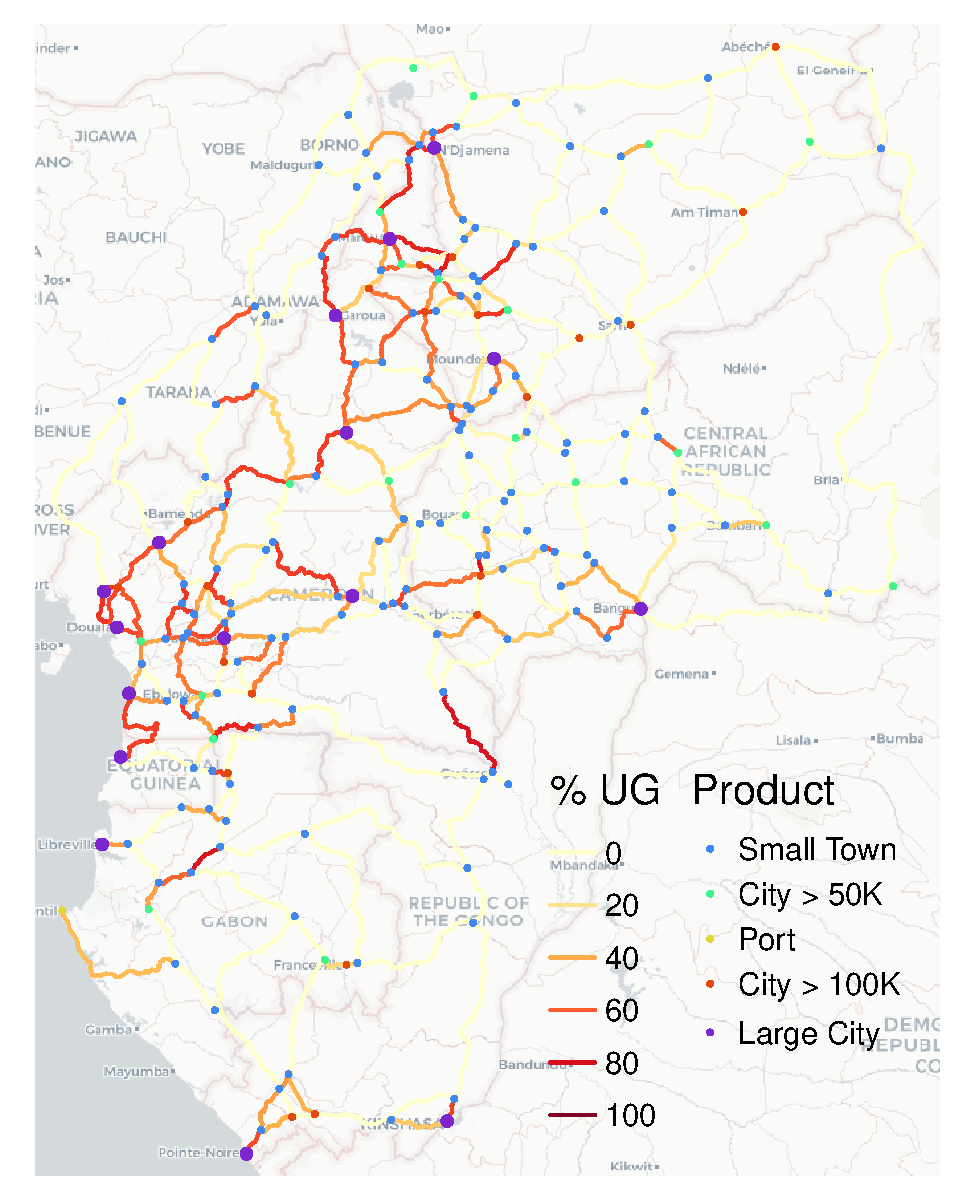
\includegraphics[width=0.38\textwidth, trim= {0.9cm 0 0.9cm 0}, clip]{"../figures/GE/trans_africa_network_GE_20g_4b_fixed_cgc_sigma3.8_rho0_julia_MACR_90kmh_google_perc_ug.pdf"}  \\
\multicolumn{3}{c}{\textbf{Inequality Aversion} ($\rho = 2$)} \\ [0.5em]
\$1B USD'15 $|$ WG: 0.4\% & \$2B USD'15 $|$ WG: 0.6\% & \$4B USD'15 $|$ WG: 0.9\%  \\
Upgraded: 1501km & Upgraded: 3057km & Upgraded: 6738km \\ 
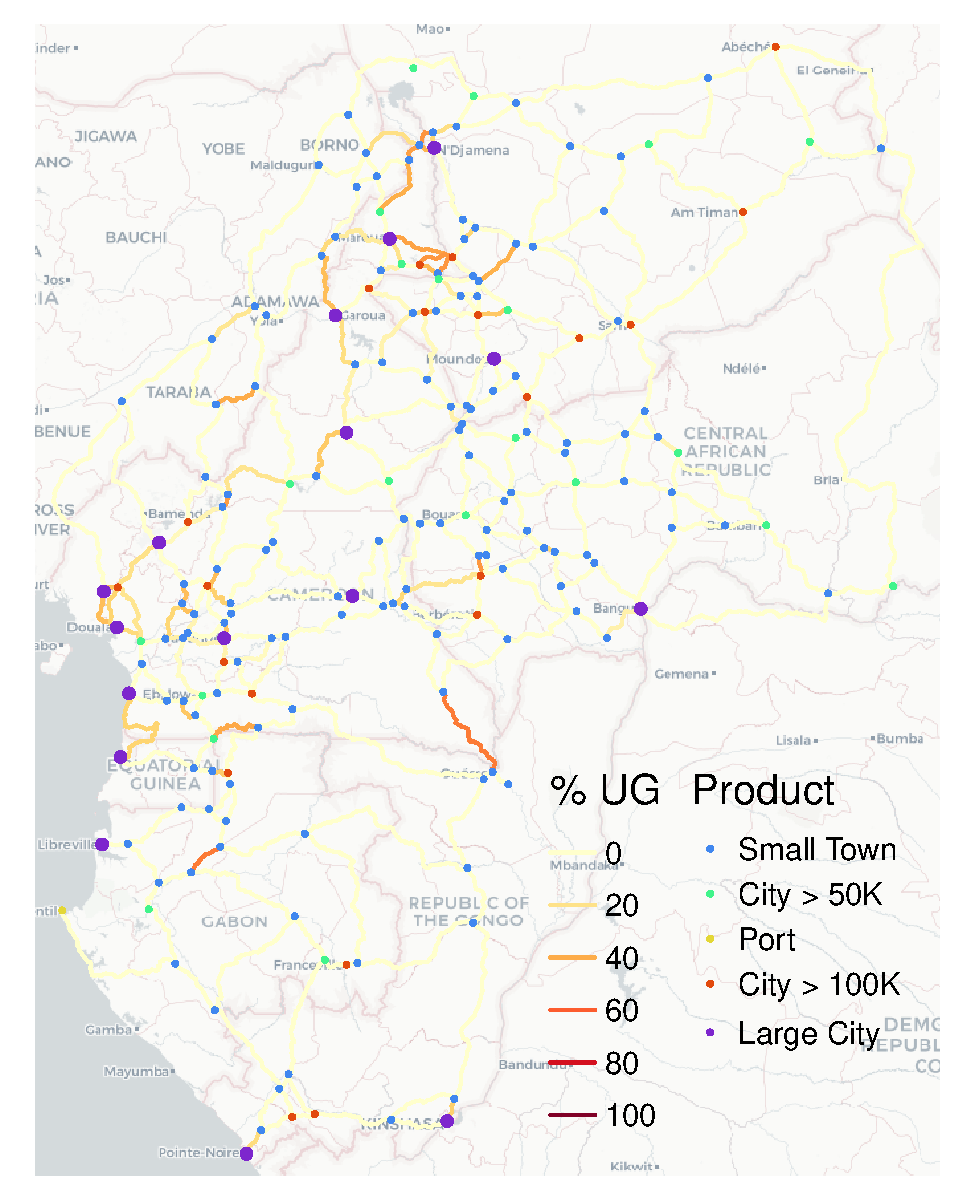
\includegraphics[width=0.38\textwidth, trim= {0.9cm 0 0.9cm 0}, clip]{"../figures/GE/trans_africa_network_GE_20g_1b_fixed_cgc_sigma3.8_rho2_julia_MACR_90kmh_google_perc_ug.pdf"} & 
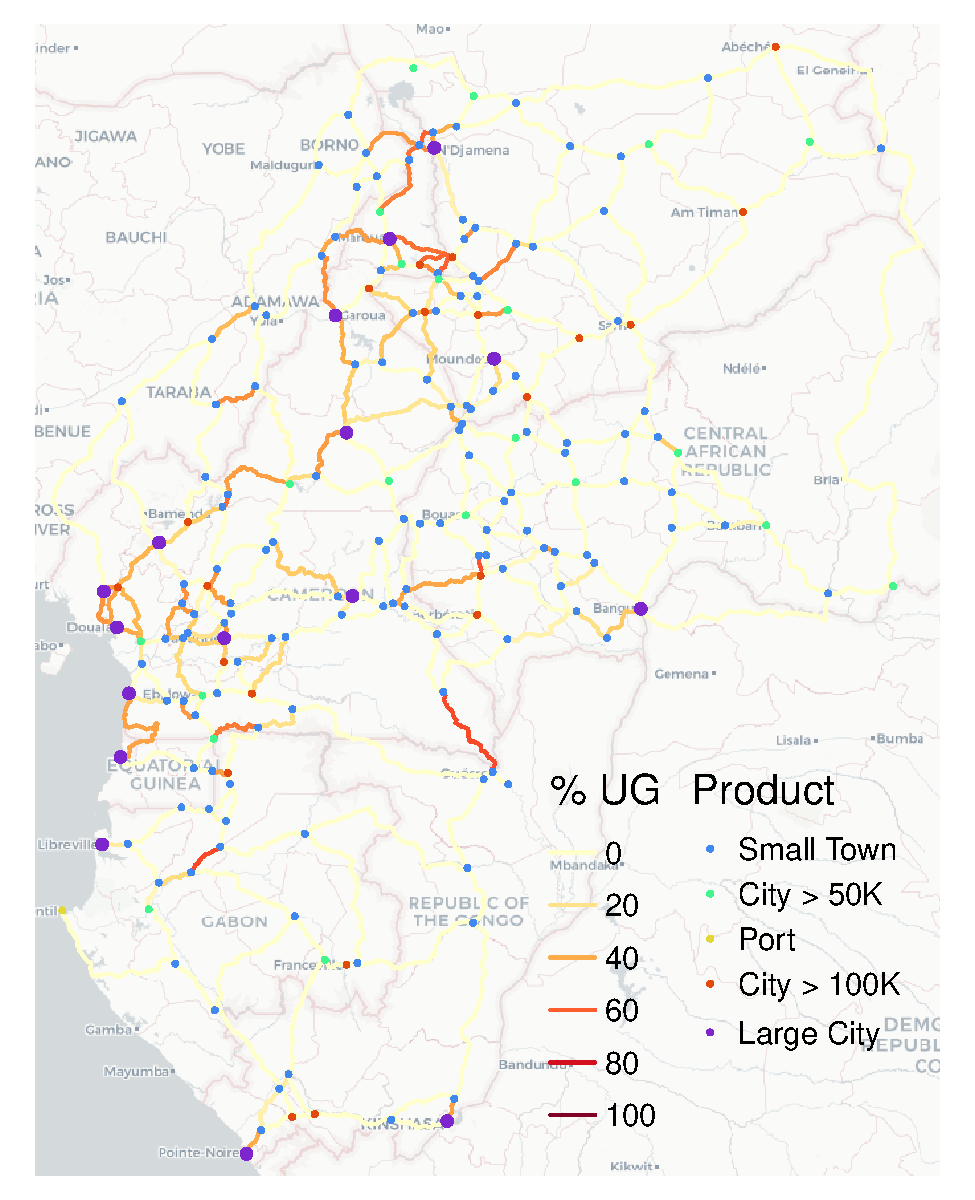
\includegraphics[width=0.38\textwidth, trim= {0.9cm 0 0.9cm 0}, clip]{"../figures/GE/trans_africa_network_GE_20g_2b_fixed_cgc_sigma3.8_rho2_julia_MACR_90kmh_google_perc_ug.pdf"} &
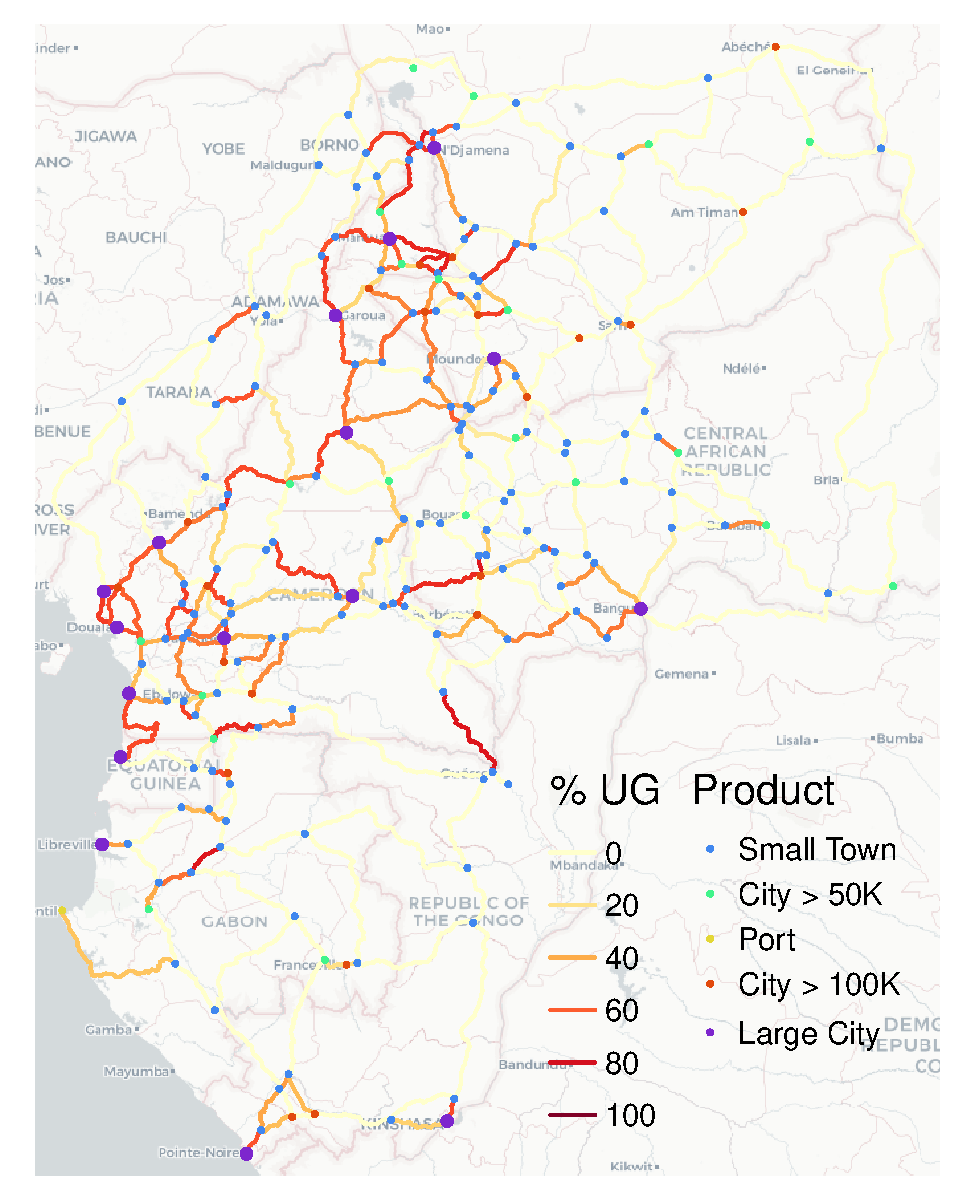
\includegraphics[width=0.38\textwidth, trim= {0.9cm 0 0.9cm 0}, clip]{"../figures/GE/trans_africa_network_GE_20g_4b_fixed_cgc_sigma3.8_rho2_julia_MACR_90kmh_google_perc_ug.pdf"}   \\
\multicolumn{3}{c}{\textbf{Increasing Returns to Infrastructure} ($\gamma^* = \gamma^2/\beta$)} \\ [0.5em]
\$1B USD'15 $|$ WG: 1.2\% & \$2B USD'15 $|$ WG: 1.8\% & \$4B USD'15 $|$ WG: 2.6\%  \\
Upgraded: 1506km & Upgraded: 3088km & Upgraded: 6682km \\ 
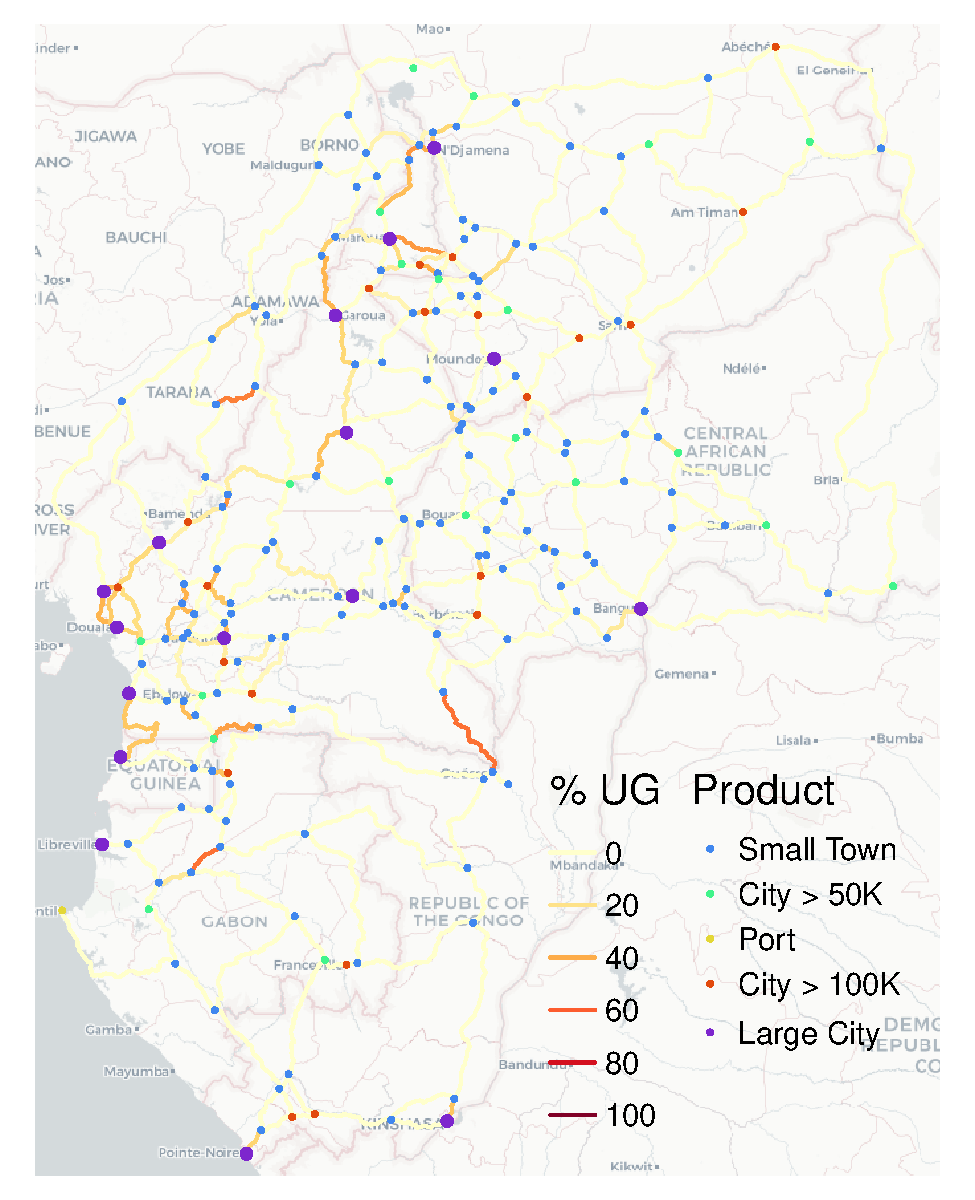
\includegraphics[width=0.38\textwidth, trim= {0.9cm 0 0.9cm 0}, clip]{"../figures/GE/trans_africa_network_GE_20g_1b_fixed_cgc_irs_sigma3.8_rho0_julia_MACR_90kmh_google_perc_ug.pdf"} & 
\includegraphics[width=0.38\textwidth, trim= {0.9cm 0 0.9cm 0}, clip]{"../figures/GE/trans_africa_network_GE_20g_2b_fixed_cgc_irs_sigma3.8_rho0_julia_MACR_90kmh_google_perc_ug.pdf"} &
\includegraphics[width=0.38\textwidth, trim= {0.9cm 0 0.9cm 0}, clip]{"../figures/GE/trans_africa_network_GE_20g_4b_fixed_cgc_irs_sigma3.8_rho0_julia_MACR_90kmh_google_perc_ug.pdf"} 
\end{tabular}
}
% \raggedright
\scriptsize 
\emph{Notes:} Figure shows the welfare maximizing 1, 2, and 4 billion USD'15 infrastructure spending on upgrading the network without border frictions for standard, inequality averse, and increasing returns planners. Spending is indicated in terms of the share (\%) of each link being upgraded $-$ planners make continuous decisions how much to spend on each link.  
\vspace{-1mm}
\end{figure}



\begin{figure}[H] \vspace{-5mm}
\centering
\caption{\label{fig:GE_UGFR} Difference in Optimal GE Spending under Frictions: Upgrading Links}
\vspace{2mm}
\resizebox{\textwidth}{!}{
\begin{tabular}{@{}c@{}c@{}c@{}} 
\$1B USD'15 $|$ \%$\Delta$WG: -1.5\% & \$2B USD'15 $|$ \%$\Delta$WG: -1.8\%  & \$4B USD'15 $|$ \%$\Delta$WG: -1.3\% \\
Upgraded: 1526km [-3km (0.2\%)] & Upgraded: 3106km [+4km (0.1\%)] & Upgraded: 6918km [+74km (1.1\%)] \\ 
\includegraphics[width=0.38\textwidth, trim= {0.9cm 0 0.9cm 0}, clip]{"../figures/GE/trans_africa_network_GE_20g_1b_fixed_cgc_sigma3.8_rho0_julia_MACR_90kmh_google_Ijk_bc_perc_ug_diff.pdf"} & 
\includegraphics[width=0.38\textwidth, trim= {0.9cm 0 0.9cm 0}, clip]{"../figures/GE/trans_africa_network_GE_20g_2b_fixed_cgc_sigma3.8_rho0_julia_MACR_90kmh_google_Ijk_bc_perc_ug_diff.pdf"} &
\includegraphics[width=0.38\textwidth, trim= {0.9cm 0 0.9cm 0}, clip]{"../figures/GE/trans_africa_network_GE_20g_4b_fixed_cgc_sigma3.8_rho0_julia_MACR_90kmh_google_Ijk_bc_perc_ug_diff.pdf"}  \\
\multicolumn{3}{c}{\textbf{Inequality Aversion} ($\rho = 2$)} \\ [0.5em]
\$1B USD'15 $|$ \%$\Delta$WG: -0.2\% & \$2B USD'15 $|$ \%$\Delta$WG: -0.7\%  & \$4B USD'15 $|$ \%$\Delta$WG: -0.8\% \\
Upgraded: 1516km [+14km (1\%)] & Upgraded: 3084km [+26km (0.9\%)] & Upgraded: 6812km [+74km (1.1\%)] \\ 
\includegraphics[width=0.38\textwidth, trim= {0.9cm 0 0.9cm 0}, clip]{"../figures/GE/trans_africa_network_GE_20g_1b_fixed_cgc_sigma3.8_rho2_julia_MACR_90kmh_google_Ijk_bc_perc_ug_diff.pdf"} & 
\includegraphics[width=0.38\textwidth, trim= {0.9cm 0 0.9cm 0}, clip]{"../figures/GE/trans_africa_network_GE_20g_2b_fixed_cgc_sigma3.8_rho2_julia_MACR_90kmh_google_Ijk_bc_perc_ug_diff.pdf"} &
\includegraphics[width=0.38\textwidth, trim= {0.9cm 0 0.9cm 0}, clip]{"../figures/GE/trans_africa_network_GE_20g_4b_fixed_cgc_sigma3.8_rho2_julia_MACR_90kmh_google_Ijk_bc_perc_ug_diff.pdf"}  \\
\multicolumn{3}{c}{\textbf{Increasing Returns to Infrastructure} ($\gamma^* = \gamma^2/\beta$)} \\ [0.5em]
\$1B USD'15 $|$ \%$\Delta$WG: -1\% & \$2B USD'15 $|$ \%$\Delta$WG: 0.2\%  & \$4B USD'15 $|$ \%$\Delta$WG: 1.7\% \\
Upgraded: 1514km [+9km (0.6\%)] & Upgraded: 3109km [+21km (0.7\%)] & Upgraded: 6781km [+98km (1.5\%)] \\ 
\includegraphics[width=0.38\textwidth, trim= {0.9cm 0 0.9cm 0}, clip]{"../figures/GE/trans_africa_network_GE_20g_1b_fixed_cgc_irs_sigma3.8_rho0_julia_MACR_90kmh_google_Ijk_bc_perc_ug_diff.pdf"} & 
\includegraphics[width=0.38\textwidth, trim= {0.9cm 0 0.9cm 0}, clip]{"../figures/GE/trans_africa_network_GE_20g_2b_fixed_cgc_irs_sigma3.8_rho0_julia_MACR_90kmh_google_Ijk_bc_perc_ug_diff.pdf"} &
\includegraphics[width=0.38\textwidth, trim= {0.9cm 0 0.9cm 0}, clip]{"../figures/GE/trans_africa_network_GE_20g_4b_fixed_cgc_irs_sigma3.8_rho0_julia_MACR_90kmh_google_Ijk_bc_perc_ug_diff.pdf"}  
\end{tabular}
}
%\resizebox{\textwidth}{!}{
%\begin{tabular}{cc}
%1B Standard Planner & 1B Inequality Averse Planner \\
%\includegraphics[width=0.48\textwidth]{"../figures/GE/trans_africa_network_GE_20g_1b_fixed_cgc_sigma3.8_rho0_julia_google_Ijk_bc_perc_ug_diff.pdf"} &
%\includegraphics[width=0.48\textwidth]{"../figures/GE/trans_africa_network_GE_20g_1b_fixed_cgc_sigma3.8_rho2_julia_google_Ijk_bc_perc_ug_diff.pdf"} \\ 
%2B Standard Planner & 2B Inequality Averse Planner \\
%\includegraphics[width=0.48\textwidth]{"../figures/GE/trans_africa_network_GE_20g_2b_fixed_cgc_sigma3.8_rho0_julia_google_Ijk_bc_perc_ug_diff.pdf"} &
%\includegraphics[width=0.48\textwidth]{"../figures/GE/trans_africa_network_GE_20g_2b_fixed_cgc_sigma3.8_rho2_julia_google_Ijk_bc_perc_ug_diff.pdf"}
%\end{tabular}
%}
% \raggedright
\scriptsize 
\emph{Notes:} Figure shows the difference in optimal spending to the frictionless case. Spending is indicated in terms of the \% of each link being upgraded. Negative (blue) spending is removed under frictions whereas positive (red) is added instead. 
% \vspace{-10cm}
\end{figure}


% \todo[inline]{To be continued...}

\begin{figure}[H] \vspace{-5mm}
\centering
\caption{\label{fig:GE_BUGNOfr} Welfare Maximizing Infrastructure Spending in GE: Building \& Upgrading Links}
\vspace{2mm}
\resizebox{\textwidth}{!}{
\begin{tabular}{@{}c@{}c@{}c@{}} 
\$1B USD'15 $|$ WG: 0.8\% & \$2B USD'15 $|$ WG: 1.1\% & \$4B USD'15 $|$ WG: 1.6\%  \\
New: 1619km $|$ UG: 120km & New: 2985km $|$ UG: 406km & New: 4819km $|$ UG: 1812km \\ 
\includegraphics[width=0.38\textwidth, trim= {0.9cm 0 0.9cm 0}, clip]{"../figures/GE/trans_africa_network_GE_add_20g_1b_fixed_cgc_sigma3.8_rho0_julia_MACR_90kmh_google_perc_ug.pdf"} & 
\includegraphics[width=0.38\textwidth, trim= {0.9cm 0 0.9cm 0}, clip]{"../figures/GE/trans_africa_network_GE_add_20g_2b_fixed_cgc_sigma3.8_rho0_julia_MACR_90kmh_google_perc_ug.pdf"} &
\includegraphics[width=0.38\textwidth, trim= {0.9cm 0 0.9cm 0}, clip]{"../figures/GE/trans_africa_network_GE_add_20g_4b_fixed_cgc_sigma3.8_rho0_julia_MACR_90kmh_google_perc_ug.pdf"}  \\
\multicolumn{3}{c}{\textbf{Inequality Aversion} ($\rho = 2$)} \\ [0.5em]
\$1B USD'15 $|$ WG: 0.8\% & \$2B USD'15 $|$ WG: 1.1\% & \$4B USD'15 $|$ WG: 1.6\%  \\
New: 1612km $|$ UG: 119km & New: 2954km $|$ UG: 419km & New: 4775km $|$ UG: 1829km \\ 
\includegraphics[width=0.38\textwidth, trim= {0.9cm 0 0.9cm 0}, clip]{"../figures/GE/trans_africa_network_GE_add_20g_1b_fixed_cgc_sigma3.8_rho2_julia_MACR_90kmh_google_perc_ug.pdf"} & 
\includegraphics[width=0.38\textwidth, trim= {0.9cm 0 0.9cm 0}, clip]{"../figures/GE/trans_africa_network_GE_add_20g_2b_fixed_cgc_sigma3.8_rho2_julia_MACR_90kmh_google_perc_ug.pdf"} &
\includegraphics[width=0.38\textwidth, trim= {0.9cm 0 0.9cm 0}, clip]{"../figures/GE/trans_africa_network_GE_add_20g_4b_fixed_cgc_sigma3.8_rho2_julia_MACR_90kmh_google_perc_ug.pdf"}  \\
\multicolumn{3}{c}{\textbf{Increasing Returns to Infrastructure} ($\gamma^* = \gamma^2/\beta$)} \\ [0.5em]
\$1B USD'15 $|$ WG: 1.3\% & \$2B USD'15 $|$ WG: 2\% & \$4B USD'15 $|$ WG: 3.1\%  \\
New: 86km $|$ UG: 1440km & New: 102km $|$ UG: 3001km & New: 285km $|$ UG: 6308km \\ 
\includegraphics[width=0.38\textwidth, trim= {0.9cm 0 0.9cm 0}, clip]{"../figures/GE/trans_africa_network_GE_add_20g_1b_fixed_cgc_irs_sigma3.8_rho0_julia_MACR_90kmh_google_perc_ug.pdf"} & 
\includegraphics[width=0.38\textwidth, trim= {0.9cm 0 0.9cm 0}, clip]{"../figures/GE/trans_africa_network_GE_add_20g_2b_fixed_cgc_irs_sigma3.8_rho0_julia_MACR_90kmh_google_perc_ug.pdf"} &
\includegraphics[width=0.38\textwidth, trim= {0.9cm 0 0.9cm 0}, clip]{"../figures/GE/trans_africa_network_GE_add_20g_4b_fixed_cgc_irs_sigma3.8_rho0_julia_MACR_90kmh_google_perc_ug.pdf"}  
\end{tabular}
%\begin{tabular}{cc}
%1B Standard Planner & 2B Standard Planner \\
%\includegraphics[width=0.48\textwidth]{"../figures/GE/trans_africa_network_GE_add_20g_1b_fixed_cgc_sigma3.8_rho0_julia_google_perc_ug.pdf"} &
%\includegraphics[width=0.48\textwidth]{"../figures/GE/trans_africa_network_GE_add_20g_2b_fixed_cgc_sigma3.8_rho0_julia_google_perc_ug.pdf"} \\ 
%1B Standard Planner: Frictions & 2B Standard Planner: Frictions \\
%\includegraphics[width=0.48\textwidth]{"../figures/GE/trans_africa_network_GE_add_20g_1b_fixed_cgc_sigma3.8_rho0_julia_google_Ijk_bc_perc_ug_diff.pdf"} &
%\includegraphics[width=0.48\textwidth]{"../figures/GE/trans_africa_network_GE_add_20g_2b_fixed_cgc_sigma3.8_rho0_julia_google_Ijk_bc_perc_ug_diff.pdf"}
%\end{tabular}
}
\raggedright
\scriptsize 
\emph{Notes:} Figure shows the welfare maximizing 1, 2, and 4 billion USD'15 infrastructure spending on building and upgrading the network without border frictions for standard, inequality averse, and increasing returns planners. Spending is indicated in terms of the share (\%) of each link being upgraded $-$ planners make continuous decisions how much to spend on each link.  
\vspace{-1mm}
\end{figure}


\begin{figure}[H] \vspace{-5mm}
\centering
\caption{\label{fig:GE_BUGFR} Difference in Optimal GE Spending under Frictions: Building \& Upgrading Links}
\vspace{2mm}
\resizebox{\textwidth}{!}{
\begin{tabular}{@{}c@{}c@{}c@{}} 
\$1B USD'15 $|$ \%$\Delta$WG: -4.9\% & \$2B USD'15 $|$ \%$\Delta$WG: -4.4\%  & \$4B USD'15 $|$ \%$\Delta$WG: -3.6\% \\
{\footnotesize $\Delta$N: 15km (1\%) $|$ $\Delta$UG: -5km (4.1\%) } & {\footnotesize $\Delta$N: 36km (1.2\%) $|$ $\Delta$UG: -19km (4.6\%)} & {\footnotesize $\Delta$N: 78km (1.6\%) $|$ $\Delta$UG: -49km (2.7\%)}  \\ 
\includegraphics[width=0.38\textwidth, trim= {0.9cm 0 0.9cm 0}, clip]{"../figures/GE/trans_africa_network_GE_add_20g_1b_fixed_cgc_sigma3.8_rho0_julia_MACR_90kmh_google_Ijk_bc_perc_ug_diff.pdf"} & 
\includegraphics[width=0.38\textwidth, trim= {0.9cm 0 0.9cm 0}, clip]{"../figures/GE/trans_africa_network_GE_add_20g_2b_fixed_cgc_sigma3.8_rho0_julia_MACR_90kmh_google_Ijk_bc_perc_ug_diff.pdf"} &
\includegraphics[width=0.38\textwidth, trim= {0.9cm 0 0.9cm 0}, clip]{"../figures/GE/trans_africa_network_GE_add_20g_4b_fixed_cgc_sigma3.8_rho0_julia_MACR_90kmh_google_Ijk_bc_perc_ug_diff.pdf"}  \\
\multicolumn{3}{c}{\textbf{Inequality Aversion} ($\rho = 2$)} \\ [0.5em]
\$1B USD'15 $|$ \%$\Delta$WG: -5.4\% & \$2B USD'15 $|$ \%$\Delta$WG: -4.8\%  & \$4B USD'15 $|$ \%$\Delta$WG: -4\% \\
{\footnotesize $\Delta$N: -8km (0.5\%) $|$ $\Delta$UG: 14km (17\%)} & {\footnotesize $\Delta$N: 6km (0.2\%) $|$ $\Delta$UG: -0.5km (0.2\%)} & {\footnotesize $\Delta$N: 72km (1.5\%) $|$ $\Delta$UG: -42km (2.4\%)}  \\  
\includegraphics[width=0.38\textwidth, trim= {0.9cm 0 0.9cm 0}, clip]{"../figures/GE/trans_africa_network_GE_add_20g_1b_fixed_cgc_sigma3.8_rho2_julia_MACR_90kmh_google_Ijk_bc_perc_ug_diff.pdf"} & 
\includegraphics[width=0.38\textwidth, trim= {0.9cm 0 0.9cm 0}, clip]{"../figures/GE/trans_africa_network_GE_add_20g_2b_fixed_cgc_sigma3.8_rho2_julia_MACR_90kmh_google_Ijk_bc_perc_ug_diff.pdf"} &
\includegraphics[width=0.38\textwidth, trim= {0.9cm 0 0.9cm 0}, clip]{"../figures/GE/trans_africa_network_GE_add_20g_4b_fixed_cgc_sigma3.8_rho2_julia_MACR_90kmh_google_Ijk_bc_perc_ug_diff.pdf"}  \\
\multicolumn{3}{c}{\textbf{Increasing Returns to Infrastructure} ($\gamma^* = \gamma^2/\beta$)} \\ [0.5em]
\$1B USD'15 $|$ \%$\Delta$WG: -1.2\% & \$2B USD'15 $|$ \%$\Delta$WG: -0.1\%  & \$4B USD'15 $|$ \%$\Delta$WG: -8.6\% \\
{\footnotesize $\Delta$N: -0.2km (0.2\%) $|$ $\Delta$UG: 9km (0.6\%) } & {\footnotesize $\Delta$N: 0.2km (0.2\%) $|$ $\Delta$UG: 19km (0.6\%)} & {\footnotesize $\Delta$N: -162km (57\%) $|$ $\Delta$UG: 350km (5.6\%)}  \\  
\includegraphics[width=0.38\textwidth, trim= {0.9cm 0 0.9cm 0}, clip]{"../figures/GE/trans_africa_network_GE_add_20g_1b_fixed_cgc_irs_sigma3.8_rho0_julia_MACR_90kmh_google_Ijk_bc_perc_ug_diff.pdf"} & 
\includegraphics[width=0.38\textwidth, trim= {0.9cm 0 0.9cm 0}, clip]{"../figures/GE/trans_africa_network_GE_add_20g_2b_fixed_cgc_irs_sigma3.8_rho0_julia_MACR_90kmh_google_Ijk_bc_perc_ug_diff.pdf"} &
\includegraphics[width=0.38\textwidth, trim= {0.9cm 0 0.9cm 0}, clip]{"../figures/GE/trans_africa_network_GE_add_20g_4b_fixed_cgc_irs_sigma3.8_rho0_julia_MACR_90kmh_google_Ijk_bc_perc_ug_diff.pdf"}  
\end{tabular}
}
%\resizebox{\textwidth}{!}{
%\begin{tabular}{cc}
%1B Standard Planner & 1B Inequality Averse Planner \\
%\includegraphics[width=0.48\textwidth]{"../figures/GE/trans_africa_network_GE_20g_1b_fixed_cgc_sigma3.8_rho0_julia_google_Ijk_bc_perc_ug_diff.pdf"} &
%\includegraphics[width=0.48\textwidth]{"../figures/GE/trans_africa_network_GE_20g_1b_fixed_cgc_sigma3.8_rho2_julia_google_Ijk_bc_perc_ug_diff.pdf"} \\ 
%2B Standard Planner & 2B Inequality Averse Planner \\
%\includegraphics[width=0.48\textwidth]{"../figures/GE/trans_africa_network_GE_20g_2b_fixed_cgc_sigma3.8_rho0_julia_google_Ijk_bc_perc_ug_diff.pdf"} &
%\includegraphics[width=0.48\textwidth]{"../figures/GE/trans_africa_network_GE_20g_2b_fixed_cgc_sigma3.8_rho2_julia_google_Ijk_bc_perc_ug_diff.pdf"}
%\end{tabular}
%}
% \raggedright
\scriptsize 
\emph{Notes:} Figure shows the difference in optimal spending to the frictionless case. Spending is indicated in terms of the \% of each link being build/upgraded. Negative (blue) spending is removed under frictions whereas positive (red) is added instead. 
% \vspace{-10cm}
\end{figure}



 \hphantom{a}
 \vspace{-8mm}

Frictions also reduce the welfare gains attainable from investing the same amount by up to 8.6\% in the \$4B IRS case. Appendix Figure \ref{fig:GE_UG_5b} shows the 5B planner's allocation, which is very similar except that this planner builds the Libreville (Kougouleu) $\to$ Bata link, even under frictions.

\section{Evaluating Regional Road Projects}

Presumably, detailed engineering knowledge was applied in the planning of road projects in the region, such as the CD13 project. However, these considerations may have insufficiently accounted for the potential economic gains and may thus be economically suboptimal or likely to not break even in the medium run. To investigate this, this final section jointly evaluates several road projects in the region using the economic modeling framework of this paper.   \newline 

Figure \ref{fig:MA_TT_PP} shows the marginal MA gains for all targeted links in the region, including gains per USD invested. In total, the projects include 6790km of planned road construction/upgrades, and their costs add up to a sum of 3.4 billion 2015 USD in my calculations following Eq. \ref{eq:COST}. They jointly yield a 28.6\% MA gain (2.14\$/min/\$), which is larger than the sum of individual marginal gains at 23.4\%, indicating that the projects jointly manage to divert more traffic along more optimal routes. Under frictions, the MA gain is 26.7\% (1.17\$/min/\$), and the sum of individual MA gains amounts to 23.2\%. Ostensibly, these planned projects include both high and low-yield links and are mainly aimed at connecting the major cities of Douala, Bangui, Brazzaville, and N'Djamena. 

\begin{figure}[H]  \vspace{-3mm}
\centering
\caption{\label{fig:MA_TT_PP} MA Gains from Regional Road Projects when Upgrading Links to $\geq$90km/h}
\vspace{2mm}
\resizebox{\textwidth}{!}{
\begin{tabular}{@{}c@{}c@{}@{}c@{}} 
No Frictions & 2019 Doing Business Frictions & MA Ratio (Frictions/Frictionless) \\ 
\includegraphics[width=0.38\textwidth, trim= {0.9cm 0 0.9cm 0}, clip]{"../figures/PE/trans_CEMAC_network_MACR_90_min_speed_perc_planned_projects.pdf"} & 
\includegraphics[width=0.38\textwidth, trim= {0.9cm 0 0.9cm 0}, clip]{"../figures/PE/trans_CEMAC_network_MACR_90_min_speed_bt_perc_planned_projects.pdf"} & 
\includegraphics[width=0.38\textwidth, trim= {0.9cm 0 0.9cm 0}, clip]{"../figures/PE/trans_CEMAC_network_MACR_90_min_speed_bt_ratio_planned_projects.pdf"} \\
\multicolumn{3}{c}{\textbf{Gains per USD'15 Invested}} \\
\includegraphics[width=0.38\textwidth, trim= {0.9cm 0 0.9cm 0}, clip]{"../figures/PE/trans_CEMAC_network_MACR_gain_all_90kmh_pusd_planned_projects.pdf"} & 
\includegraphics[width=0.38\textwidth, trim= {0.9cm 0 0.9cm 0}, clip]{"../figures/PE/trans_CEMAC_network_MACR_gain_all_90kmh_pusd_bt_planned_projects.pdf"} & 
\includegraphics[width=0.38\textwidth, trim= {0.9cm 0 0.9cm 0}, clip]{"../figures/PE/trans_CEMAC_network_MACR_gain_all_90kmh_pusd_bt_ratio_planned_projects.pdf"}
\end{tabular}
}
%\begin{tabular}{cc}
%No Frictions & 2019 Doing Business Frictions \\
%\includegraphics[width=0.48\textwidth]{"../figures/PE/trans_CEMAC_network_MA_100_min_speed_perc_planned_projects.pdf"} &
%\includegraphics[width=0.48\textwidth]{"../figures/PE/trans_CEMAC_network_MA_100_min_speed_bt_perc_planned_projects.pdf"}  \\ [-0.2em]
%\end{tabular}
\raggedright
\scriptsize 
\emph{Notes:} Figure shows total travel-time-denominated MA gains measured (summed) across all trips from upgrading a link to allow travel speeds of $\geq$90km/h for investment projects in the region. The bottom panel shows marginal returns in \$/min/\$ (dollar per minute (MA) per dollar invested; dollars are in constant 2015 terms).  \vspace{-5mm}
\end{figure}

%\begin{figure}[H]  \vspace{-1mm}
%\centering
%\caption{\label{fig:MA_TT_PUSD} Investment Returns in \$/min/\$ from Building/Upgrading Each Link to $\geq$90km/h}
%\vspace{2mm}
%\begin{tabular}{cc}
%No Frictions & 2019 Doing Business Frictions \\
%\includegraphics[width=0.48\textwidth]{"../figures/PE/trans_CEMAC_network_MA_gain_all_100kmh_pusd_planned_projects.pdf"} &
%\includegraphics[width=0.48\textwidth]{"../figures/PE/trans_CEMAC_network_MA_gain_all_100kmh_pusd_bt_planned_projects.pdf"}  \\ [-0.2em]
%\end{tabular}
%\raggedright
%\scriptsize 
%\emph{Notes:} Figure shows marginal returns in \$/min/\$ (dollar per minute $=$ MA per dollar invested) from upgrading a link to allow travel speeds of $\geq$km/h or building a new link for road investment projects in the region.
% % \vspace{-2mm}
%\end{figure}

Take as a comparison the PE package with high-yield links $>$1\$/min/\$ without border frictions on the RHS of Figure \ref{fig:UG_cons}. It costs \$4B, which is slightly more than the \$3.4B regional projects but yields a 44\% MA gain or 2.8\$/min/\$ (1.7\$/min/\$ under frictions), which is larger than the 28.6\% MA gain at 2.14\$/min/\$ from the regional projects. The main difference is that the optimal PE package upgrades many more links in the Douala-Yaounde region and further north in the high-crop yield areas between Maroua and Moundou but no links around Bangui in CAR. \newline 

A further relevant question is whether these road projects are welfare-maximizing. Eyeballing the allocations of the 4 billion USD'15 GE planners in Figures \ref{fig:GE_UGNOfr} and \ref{fig:GE_BUGNOfr} indicates that these planners spend more in the Douala-Yaounde region where many people live, and in the north connecting to N'Djamena and the crop regions around Maroua. To be sure, I also simulate a \$3.4 billion USD'15 planner without frictions. For simulations where the planner is only allowed to upgrade, I leave out the planned new link between Ouesso and Mbaiki, which is 420km long and costs 200 million USD'15, thus shrinking the budget to \$3.2B. Figure \ref{fig:GE_UG_Proj} reports the results. 



\begin{figure}[H] \vspace{-2mm}
\centering
\caption{\label{fig:GE_UG_Proj} Welfare Maximizing Infrastructure Spending in GE: Project Equivalent (\$3.4B)}
\vspace{2mm}
\resizebox{\textwidth}{!}{
\begin{tabular}{@{}c@{}c@{}c@{}} 
\textbf{Only Upgrading} & \textbf{Inequality Aversion} & \textbf{Building \& Upgrading} \\ 
Upgraded: 5295km$|$ WG: 0.9\% & Upgraded: 5216km $|$ WG: 0.8\% & N: 4453km, UG: 1228km $|$ WG: 1.5\% \\ 
\includegraphics[width=0.38\textwidth, trim= {0.9cm 0 0.9cm 0}, clip]{"../figures/GE/trans_africa_network_GE_20g_3200m_fixed_cgc_sigma3.8_rho0_julia_MACR_90kmh_google_perc_ug.pdf"} & 
\includegraphics[width=0.38\textwidth, trim= {0.9cm 0 0.9cm 0}, clip]{"../figures/GE/trans_africa_network_GE_20g_3200m_fixed_cgc_sigma3.8_rho2_julia_MACR_90kmh_google_perc_ug.pdf"} &
\includegraphics[width=0.38\textwidth, trim= {0.9cm 0 0.9cm 0}, clip]{"../figures/GE/trans_africa_network_GE_add_20g_3400m_fixed_cgc_sigma3.8_rho0_julia_MACR_90kmh_google_perc_ug.pdf"} \\
\multicolumn{3}{c}{\textbf{Increasing Returns to Infrastructure} ($\gamma^* = \gamma^2/\beta$)} \\ [0.5em]
Upgraded: 5211km $|$ WG: 2.3\% & Upgraded: 5218km $|$ WG: 2.3\% & N: 273km, UG: 5233km $|$ WG: 2.9\% \\ 
\includegraphics[width=0.38\textwidth, trim= {0.9cm 0 0.9cm 0}, clip]{"../figures/GE/trans_africa_network_GE_20g_3200m_fixed_cgc_irs_sigma3.8_rho0_julia_MACR_90kmh_google_perc_ug.pdf"} & 
\includegraphics[width=0.38\textwidth, trim= {0.9cm 0 0.9cm 0}, clip]{"../figures/GE/trans_africa_network_GE_20g_3200m_fixed_cgc_irs_sigma3.8_rho2_julia_MACR_90kmh_google_perc_ug.pdf"} &
\includegraphics[width=0.38\textwidth, trim= {0.9cm 0 0.9cm 0}, clip]{"../figures/GE/trans_africa_network_GE_add_20g_3400m_fixed_cgc_irs_sigma3.8_rho0_julia_MACR_90kmh_google_perc_ug.pdf"} \\
\end{tabular}
%\begin{tabular}{cc}
%Standard Planner & Standard Planner: Frictions \\
%\includegraphics[width=0.48\textwidth]{"../figures/GE/trans_africa_network_GE_20g_2327m_fixed_cgc_sigma3.8_rho0_julia_google_perc_ug.pdf"} &
% \includegraphics[width=0.48\textwidth]{"../figures/GE/trans_africa_network_GE_20g_2327m_fixed_cgc_sigma3.8_rho0_julia_google_Ijk_bc_perc_ug_diff.pdf"} 
%\end{tabular}
}
% \raggedright
\scriptsize 
\emph{Notes:} Figure shows the welfare maximizing spending of 3.4 billion USD'15 (equivalent to the cost of all regional road projects) on the network without border frictions. Spending is indicated in terms of the \% of each link being upgraded. 
 \vspace{-1mm}
\end{figure}

The welfare maximizing allocations are very similar to the 4 billion USD'15 planners overall. Significant building/upgrading of roads towards/around Bangui in CAR is not welfare maximizing, considering where most people live and where most economic value, including crop yield, is produced. Nevertheless, and in contrast to the PE package, all GE planners improve connectivity between Bangui and Brazzaville, particularly links connecting to Ouesso in Congo. \newline 


At last, repeating the reverse-PDV calculation from Table \ref{tab:MACAB} yields that the planned projects would be jointly profitable in PDV terms if they raise the macroeconomic growth rate by 0.74\% in the 3.5\% baseline growth scenario or by 1.62\% in the 2\% baseline growth scenario. \newline 




\section{Summary and Conclusion} 

Analyzing the road network of the CEMAC region and optimal investments into it following the methodology of \citet{krantz2024optimal} yields rich and detailed insights into local and regional investment potentials in partial and general equilibrium. \newline 

The first general insight is that borders in the region are thick, and friction should duly be reduced. Eliminating all border controls/costs would increase travel time-denominated market access (MA) by 58\% and distance-denominated MA by 44\%. This must be compared to a 64\% MA gain from upgrading all roads to 90km/h and a cost of \$19B USD'15 and a 72\% MA gain from upgrades combined with additional \$8B USD'15 investments in new links. It is clear that the region's thick borders and trade regulations are a major bottleneck and should be reduced first. \newline 

Of particular significance are borders into Cameroon, which is the region's largest economy at 46\% of CEMAC GDP and 45\% of CEMAC population. Which border post to focus on depends on the navigational properties of the network. My simulations yield that reducing the border at Garoua-Boulai (CMR) would yield the highest MA gains. According to the 2019 business survey and \citet{krantz2024optimal}, borders between Cameroon and CAR have an average cost equivalent to 1592km of road distance or 112h of road time. A 50\% reduction of the border at Garoua-Boulai, considering traders' optimizing behavior, would yield a 1.8\% increase in the region's MA. Reducing the border by 90\% to 12h road equivalent could raise MA by as much as 8.1\%. \newline  

Apart from thick borders, many links are slow, at a median speed of 60km/h, and need upgrading. Upgrading roads near populated areas in Cameroon (Douala and Yaounde) and Brazzaville, Point-Noire, and N'Djamena yields high MA and welfare gains relative to the costs. Much can also be gained from building new links that increase route efficiency. Particularly to mention here is better connecting Equatorial Guinea (Bata) to the north (Kiribi) and south (Libreville), and Libreville to Port-Gentil in Gabon. \newline 

\$4B-\$5B USD'15 high-yield-links road packages can yield 43\%-53\% MA gains and should be highly profitable in the medium run (30-year PDV profitability requires 1\% increase in macroeconomic growth rate at 3.5\% baseline growth). Planned road projects in the region, such as CD13, are estimated to cost \$3.4B USD'15 and yield 27-29\% MA gains (1.2-2.1\$/min/\$). Compared to gains of 1.4-2.8\$/min/\$ for the \$4B-\$5B PE packages, these are modestly economically suboptimal but manage to better connect some remote regions around Bangui/CAR. Optimal investments stipulate more connectivity improvements around populated and agricultural areas, particularly in Cameroon, but also up north towards N'Djamena and between the coastal cities. These are of higher value as more people benefit from them than long-distance roads in remote areas. \newline 

A final notable finding is that under standard decreasing returns assumption (strong congestion forces), GE planners invest $>$70\% of their budget on constructing new links, despite such links being more expensive than upgrading existing ones. This stands in contrast to results for the entire African network \citep{krantz2024optimal}, where planners invest $\sim$70\% in upgrading, indicating that particularly in the CEMAC region, much can be gained by increasing the network route efficiency through new roads. Under increasing returns to infrastructure (weak congestion forces), however, planners only build a few new links between coastal cities and invest more than 95\% of their budget in upgrading. It is thus vital to estimate the size of congestion parameters for inter-city transport in Africa. So far, only estimates within cities are available. Congestion forces are presumably much weaker in inter-city transport. 
 
%   	\item Road investments in Cameroon (Douala-Yaounde and up north toward N'Djamena) and in borders crossing to Cameroon yield greatest marginal benefits (Cameroon $=$ 46\% of CEMAC GDP and 45\% of CEMAC population).
%  	\item 100\% border frictions reduction yields 58\% MA gain, vs. 64\% gain from upgrades to 90km/h (\$19B USD'15) and 72\% from upgrades + \$8B USD'15 new links. 
%  	\item \$4B-\$5B USD'15 high-yield-links road packages (or below) can yield 43\%-53\% MA gains and should be highly-profitable in medium run (30-year PDV profitability requires 1\% increase in macroeconomic growth rate at 3.5\% baseline growth). 
%  	\item Planned works estimated at \$3.4B USD'15 yield 27-29\% MA gain (1.2-2.1\$/min/\$ vs. 1.4-2.8\$/min/\$ for the \$4B-\$5B PE packages) $\to$ modest inefficiency.
%    \item GE planners invest more in new links than upgrades if given the choice - unlike Africa \citep{krantz2024optimal} $\to$ strong indication that network needs to be expanded. (Also: inequality averse planners invest more in poorer north (Chad, CAR)).

% Their short-term economic returns may thus be called into question. High-yield upgrading packages around the aforementioned urban centers on the other hand yield sizeable economic returns in both the short and medium run that are likely to outweigh project costs.  % in light of what could be gained by better connecting populated areas. 


\newpage

\bibliographystyle{apacite}
\bibliography{bibliography} % This links to a file bibliography.bib with the citations

\newpage
\section*{Appendix}

\begin{figure}[H] \vspace{-1mm}
\centering
\caption{\label{fig:ACLED} ACLED Armed Conflict Events 2018-2014} 
\vspace{2mm}
\includegraphics[width=0.9\textwidth]{"../figures/ACLED_CEMAC_FATALITIES.pdf"} \\
% \raggedright
\scriptsize 
\emph{Notes:} Figure shows ACLED \citep{raleigh2023political} armed conflict events between 2018 and 2024.
% \vspace{-2mm}
\end{figure}

\begin{figure}[h!] \vspace{-2mm}
\centering
\caption{\label{fig:GE_UGNOfr_5b} Welfare Maximizing Infrastructure Spending in GE: Upgrading Links with 5 Billion 2015 USD Planning Budget}
\vspace{2mm}
\resizebox{\textwidth}{!}{
\begin{tabular}{@{}c@{}c@{}c@{}} 
\textbf{Standard Planner} & \textbf{IA Planner} ($\rho = 2$) & \textbf{IRS Planner} ($\gamma^* = \gamma^2/\beta$) \\
Upgraded: 8869km $|$ WG: 1.1\% & Upgraded: 8652km $|$ WG: 1.08\% &  Upgraded: 8567km $|$ WG: 3\%  \\
\includegraphics[width=0.38\textwidth, trim= {0.9cm 0 0.9cm 0}, clip]{"../figures/GE/trans_africa_network_GE_20g_5b_fixed_cgc_sigma3.8_rho0_julia_MACR_90kmh_google_perc_ug.pdf"} & 
\includegraphics[width=0.38\textwidth, trim= {0.9cm 0 0.9cm 0}, clip]{"../figures/GE/trans_africa_network_GE_20g_5b_fixed_cgc_sigma3.8_rho2_julia_MACR_90kmh_google_perc_ug.pdf"} &
\includegraphics[width=0.38\textwidth, trim= {0.9cm 0 0.9cm 0}, clip]{"../figures/GE/trans_africa_network_GE_20g_5b_fixed_cgc_irs_sigma3.8_rho0_julia_MACR_90kmh_google_perc_ug.pdf"}  \\
{\small $\Delta$UG: +93km (1.1\%) $|$ \%$\Delta$WG: -0.9\%} & {\small $\Delta$UG: +118km (1.4\%) $|$ \%$\Delta$WG: -0.4\%} &  {\small $\Delta$UG: +114km (1.3\%) $|$ \%$\Delta$WG: 0.6\%} \\
\includegraphics[width=0.38\textwidth, trim= {0.9cm 0 0.9cm 0}, clip]{"../figures/GE/trans_africa_network_GE_20g_5b_fixed_cgc_sigma3.8_rho0_julia_MACR_90kmh_google_Ijk_bc_perc_ug_diff.pdf"} & 
\includegraphics[width=0.38\textwidth, trim= {0.9cm 0 0.9cm 0}, clip]{"../figures/GE/trans_africa_network_GE_20g_5b_fixed_cgc_sigma3.8_rho2_julia_MACR_90kmh_google_Ijk_bc_perc_ug_diff.pdf"} &
\includegraphics[width=0.38\textwidth, trim= {0.9cm 0 0.9cm 0}, clip]{"../figures/GE/trans_africa_network_GE_20g_5b_fixed_cgc_irs_sigma3.8_rho0_julia_MACR_90kmh_google_Ijk_bc_perc_ug_diff.pdf"}  
\end{tabular}
}
%
%5B Standard Planner & 5B Inequality Averse Planner \\
%\includegraphics[width=0.48\textwidth]{"../figures/GE/trans_africa_network_GE_20g_5b_fixed_cgc_sigma3.8_rho0_julia_google_perc_ug.pdf"} &
%\includegraphics[width=0.48\textwidth]{"../figures/GE/trans_africa_network_GE_20g_5b_fixed_cgc_sigma3.8_rho2_julia_google_perc_ug.pdf"} \\
%5B Standard Planner: Frictions & 5B Inequality Averse Planner: Frictions \\
%\includegraphics[width=0.48\textwidth]{"../figures/GE/trans_africa_network_GE_20g_5b_fixed_cgc_sigma3.8_rho0_julia_google_Ijk_bc_perc_ug_diff.pdf"} &
%\includegraphics[width=0.48\textwidth]{"../figures/GE/trans_africa_network_GE_20g_5b_fixed_cgc_sigma3.8_rho2_julia_google_Ijk_bc_perc_ug_diff.pdf"}
%\end{tabular}
%}
% \raggedright
\scriptsize 
\emph{Notes:} Figure shows the welfare maximizing 5 billion USD'15 infrastructure spending on upgrading the network without border frictions (top) and with border frictions (bottom). Spending is indicated in \% of each link being upgraded $-$ planners make continuous spending decisions. Under frictions (bottom) the difference to the frictionless case is shown.   
% \vspace{-10cm}
\end{figure}



\begin{figure}[h!] \vspace{-2mm}
\centering
\caption{\label{fig:GE_UG_5b} Welfare Maximizing Infrastructure Spending in GE: Building and Upgrading Links with 5 Billion 2015 USD Planning Budget}
\vspace{2mm}
\resizebox{\textwidth}{!}{
\begin{tabular}{@{}c@{}c@{}c@{}} 
\textbf{Standard Planner} & \textbf{IA Planner} ($\rho = 2$) & \textbf{IRS Planner} ($\gamma^* = \gamma^2/\beta$) \\
{\small N: 5607km $|$ UG: 2635km $|$ WG: 1.8\%} & {\small N: 5544km $|$ UG: 2655km $|$ WG: 1.8\%} &  {\small N: 319km $|$ UG: 8137km $|$ WG: 3.5\%}  \\
\includegraphics[width=0.38\textwidth, trim= {0.9cm 0 0.9cm 0}, clip]{"../figures/GE/trans_africa_network_GE_add_20g_5b_fixed_cgc_sigma3.8_rho0_julia_MACR_90kmh_google_perc_ug.pdf"} & 
\includegraphics[width=0.38\textwidth, trim= {0.9cm 0 0.9cm 0}, clip]{"../figures/GE/trans_africa_network_GE_add_20g_5b_fixed_cgc_sigma3.8_rho2_julia_MACR_90kmh_google_perc_ug.pdf"} &
\includegraphics[width=0.38\textwidth, trim= {0.9cm 0 0.9cm 0}, clip]{"../figures/GE/trans_africa_network_GE_add_20g_5b_fixed_cgc_irs_sigma3.8_rho0_julia_MACR_90kmh_google_perc_ug.pdf"}  \\
{\footnotesize $\Delta$N: 66km $|$ $\Delta$UG: -42km $|$ \%$\Delta$WG: -3.6\%} & {\footnotesize $\Delta$N: 90km $|$ $\Delta$UG: -38km $|$ \%$\Delta$WG: -3.8\%} & {\footnotesize $\Delta$N: 32km $|$ $\Delta$UG: 91km $|$ \%$\Delta$WG: -0.8\%} \\
\includegraphics[width=0.38\textwidth, trim= {0.9cm 0 0.9cm 0}, clip]{"../figures/GE/trans_africa_network_GE_add_20g_5b_fixed_cgc_sigma3.8_rho0_julia_MACR_90kmh_google_Ijk_bc_perc_ug_diff.pdf"} & 
\includegraphics[width=0.38\textwidth, trim= {0.9cm 0 0.9cm 0}, clip]{"../figures/GE/trans_africa_network_GE_add_20g_5b_fixed_cgc_sigma3.8_rho2_julia_MACR_90kmh_google_Ijk_bc_perc_ug_diff.pdf"} 
&
\includegraphics[width=0.38\textwidth, trim= {0.9cm 0 0.9cm 0}, clip]{"../figures/GE/trans_africa_network_GE_add_20g_5b_fixed_cgc_irs_sigma3.8_rho0_julia_MACR_90kmh_google_Ijk_bc_perc_ug_diff.pdf"}  
\end{tabular}
}
%\begin{tabular}{cc}
%5B Standard Planner & 5B Standard Planner: Frictions \\
%\includegraphics[width=0.48\textwidth]{"../figures/GE/trans_africa_network_GE_add_20g_5b_fixed_cgc_sigma3.8_rho0_julia_google_perc_ug.pdf"} &
% \includegraphics[width=0.48\textwidth]{"../figures/GE/trans_africa_network_GE_add_20g_5b_fixed_cgc_sigma3.8_rho0_julia_google_Ijk_bc_perc_ug_diff.pdf"} 
%\end{tabular}
% \raggedright
\scriptsize 
\emph{Notes:} Figure shows the welfare maximizing 5 billion USD'15 infrastructure spending on building and upgrading the network without border frictions (top) and with border frictions (bottom). Spending is indicated in \% of each link being upgraded $-$ planners make continuous spending decisions. Under frictions (bottom) the difference to the frictionless case is shown.   
% \vspace{-10cm}
\end{figure}



\begin{figure}[h!] \vspace{-8mm}
\centering
\caption{\label{fig:GE_UGNOfrFL} Flow of Goods under Optimal 2B Investments: Upgrading Links}
\vspace{2mm}
\begin{tabular}{c}
\includegraphics[width=\textwidth]{"../figures/GE/trans_africa_network_GE_20g_2b_fixed_cgc_sigma3.8_rho0_julia_MACR_90kmh_google_good_flows_4_city.pdf"} \\
% Standard Planner: With Frictions \\
% \includegraphics[width=\textwidth]{"../figures/GE/trans_africa_network_GE_20g_2b_fixed_cgc_sigma3.8_rho0_bc_julia_MACR_90kmh_google_good_flows_4_city.pdf"} \\
\textbf{Inequality Aversion} ($\rho = 2$) \\
\includegraphics[width=\textwidth]{"../figures/GE/trans_africa_network_GE_20g_2b_fixed_cgc_sigma3.8_rho2_julia_MACR_90kmh_google_good_flows_4_city.pdf"} \\
\textbf{Increasing Returns to Infrastructure} ($\gamma^* = \gamma^2/\beta$) \\
\includegraphics[width=\textwidth]{"../figures/GE/trans_africa_network_GE_20g_2b_fixed_cgc_irs_sigma3.8_rho0_julia_MACR_90kmh_google_good_flows_4_city.pdf"} 
\end{tabular}
% \raggedright
\scriptsize 
\emph{Notes:} Figure shows the flow of goods from selected cities under optimal 2B upgrading investments on a log scale. \\ \vspace{-20mm}
\end{figure}

\begin{figure}[h!] \vspace{-4mm}
\centering
\caption{\label{fig:GE_BUGNOfrFL} Flow of Goods under Optimal 2B Investments: Building \& Upgrading Links}
\vspace{2mm}
\begin{tabular}{c}
\includegraphics[width=\textwidth]{"../figures/GE/trans_africa_network_GE_add_20g_2b_fixed_cgc_sigma3.8_rho0_julia_MACR_90kmh_google_good_flows_4_city.pdf"} \\
\textbf{Inequality Aversion} ($\rho = 2$) \\
\includegraphics[width=\textwidth]{"../figures/GE/trans_africa_network_GE_add_20g_2b_fixed_cgc_sigma3.8_rho2_julia_MACR_90kmh_google_good_flows_4_city.pdf"} \\
\textbf{Increasing Returns to Infrastructure} ($\gamma^* = \gamma^2/\beta$) \\
\includegraphics[width=\textwidth]{"../figures/GE/trans_africa_network_GE_add_20g_2b_fixed_cgc_irs_sigma3.8_rho0_julia_MACR_90kmh_google_good_flows_4_city.pdf"} 
%1B Standard Planner \\
%\includegraphics[width=\textwidth]{"../figures/GE/trans_africa_network_GE_add_20g_1b_fixed_cgc_sigma3.8_rho0_julia_google_good_flows_4_city.pdf"} \\
%1B Standard Planner: With Frictions \\
%\includegraphics[width=\textwidth]{"../figures/GE/trans_africa_network_GE_add_20g_1b_fixed_cgc_sigma3.8_rho0_bc_julia_google_good_flows_4_city.pdf"} \\
%2B Standard Planner \\
%\includegraphics[width=\textwidth]{"../figures/GE/trans_africa_network_GE_add_20g_2b_fixed_cgc_sigma3.8_rho0_julia_google_good_flows_4_city.pdf"} \\
%2B Standard Planner: With Frictions \\
%\includegraphics[width=\textwidth]{"../figures/GE/trans_africa_network_GE_20g_2b_fixed_cgc_sigma3.8_rho0_bc_julia_google_good_flows_4_city.pdf"} \\
\end{tabular}
% \raggedright
\scriptsize 
\emph{Notes:} Figure shows the flow of goods from selected cities under optimal 2B road building and upgrading investments on a log scale.
\end{figure}




\end{document}